\chapter{Control distributions}

Kinematic distributions after all cuts (Section \ref{chap:EventSelection}) and corrections applied on MC (Section \ref{chap:MCCor}), are presented in this chapter. Distributions for $W \to l\nu$ are split in charge and shown on a Figs. \ref{ris:WlnuLep}- \ref{ris:WlnumtWM}. Distributions for $Z \to l^{+}l^{-}$ analysis are shown on a Fig. \ref{ris:Zll}-\ref{ris:Zll2}.  

These plots also showing the systematic and statistical uncertainty as a shaded band. The uncertainties are including all sources, described in a \ref{chap:Unc}, except for uncertainties coming from shape variation due to a PDF reweighing and QCD background and luminosity.  All uncorrelated uncertainty sources are summed in quadrature. The expected background contributions are estimated using MC simulations, apart from QCD background, which is found with a data driven method, as explained in a previous chapter.

Good overall agreement between data and MC is observed.


%============================================================================================================
% Lep Eta

\begin{figure}[h]
\begin{minipage}[h]{0.49\linewidth}
\center{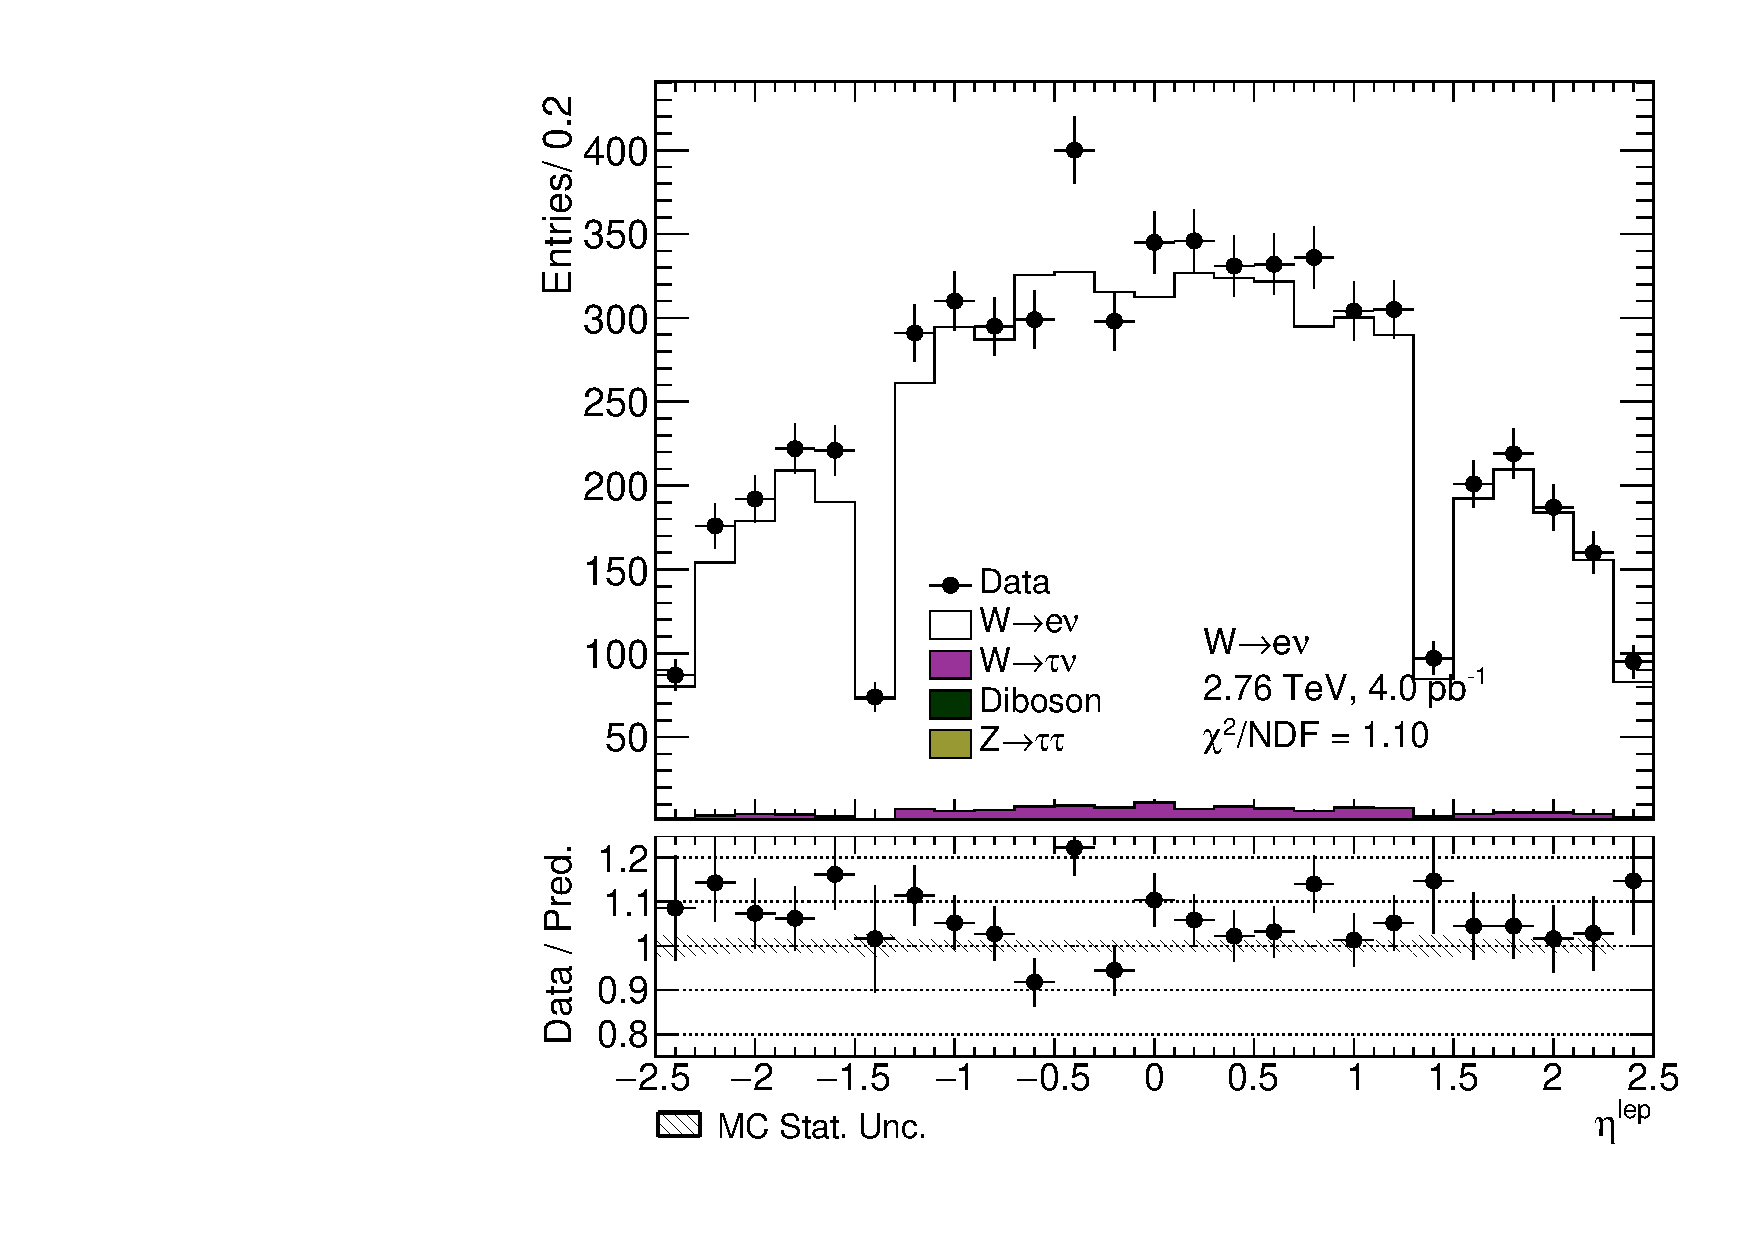
\includegraphics[width=1.\linewidth]{ControlPlots/Wanalysis/W_Boson_lepEta.pdf} \\ a)}
\end{minipage}
\hfill
\begin{minipage}[h]{0.49\linewidth}
\center{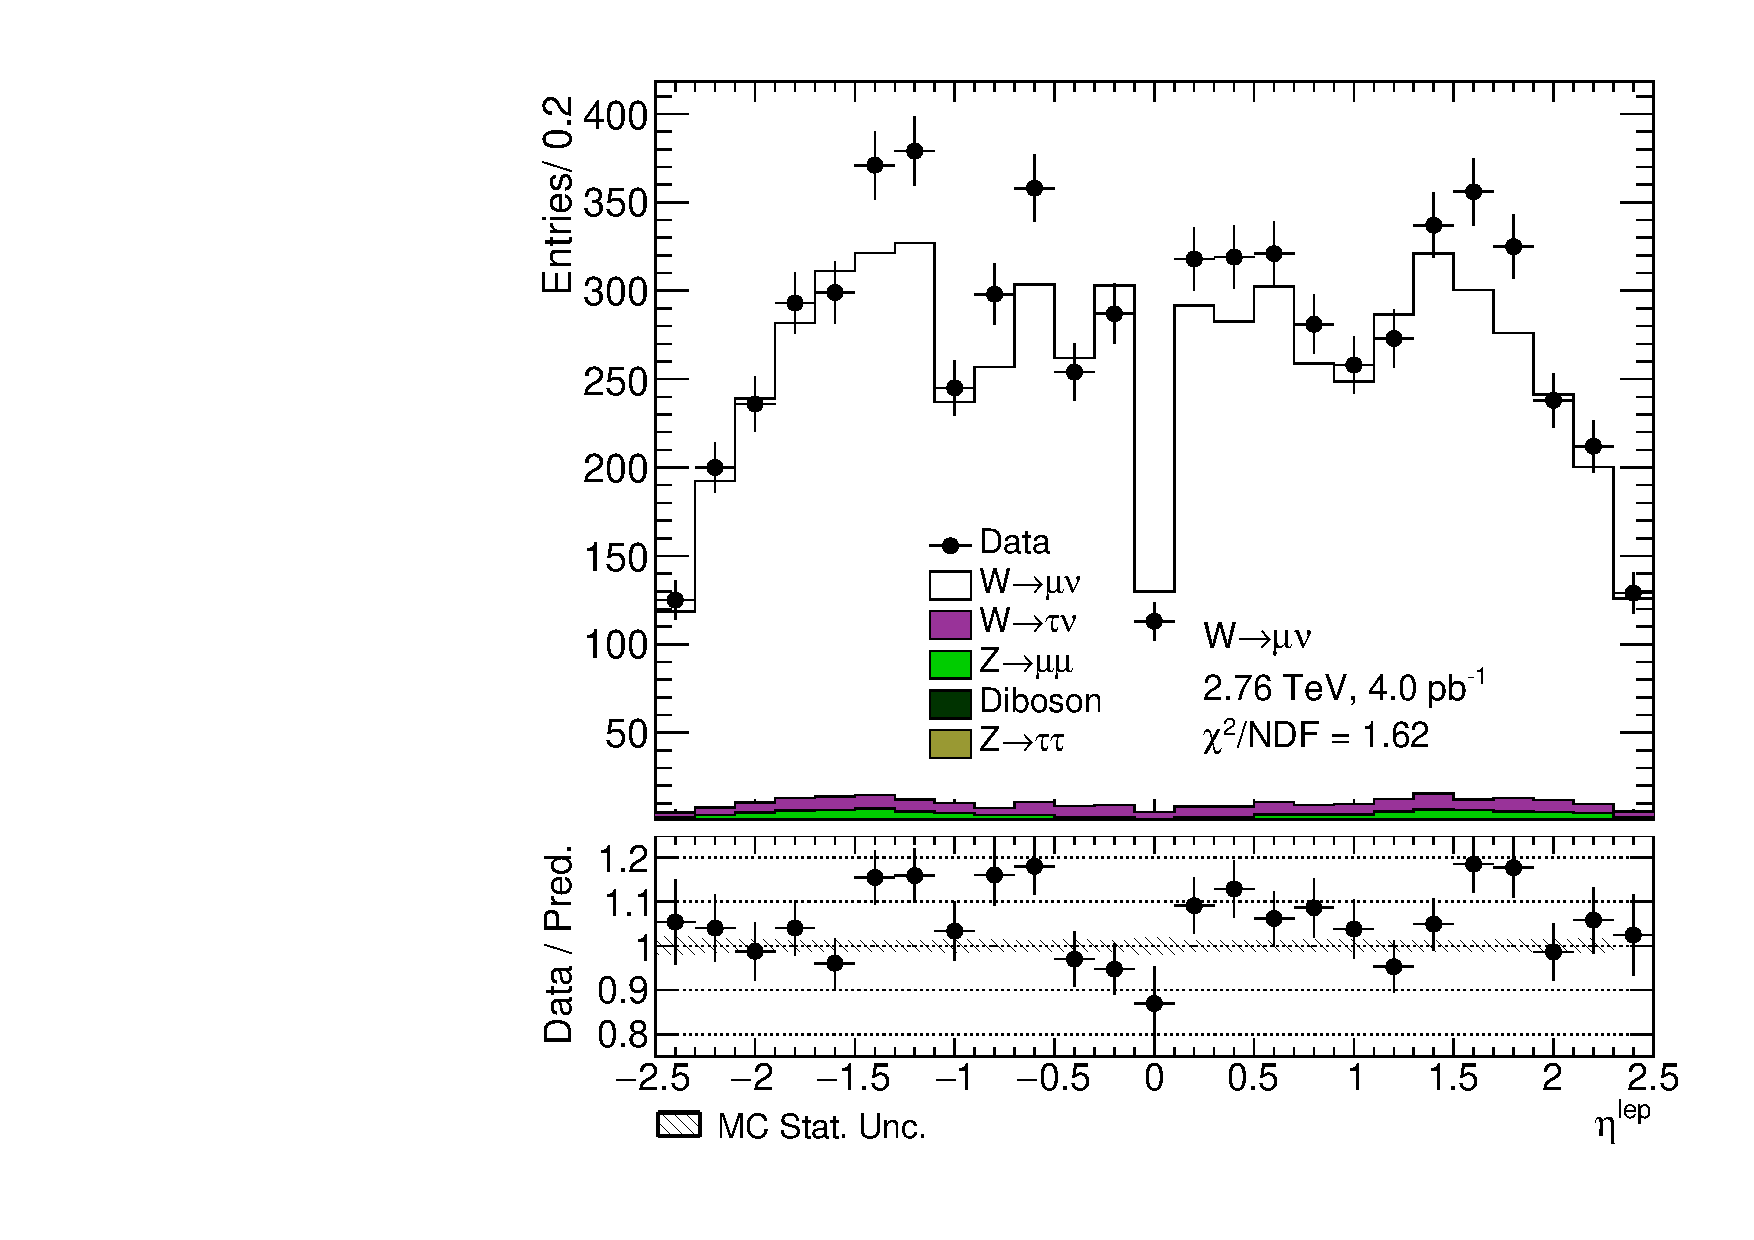
\includegraphics[width=1.\linewidth]{ControlPlots/Wanalysis/Wmu_Boson_lepEta.pdf} \\ b)}
\end{minipage}
\caption{Lepton pseudorapidity distribution from the a) \wenu selection and  b) the \wmunu selection.}
\label{ris:WlnuLep}
\end{figure}

\begin{figure}[h]
\begin{minipage}[h]{0.49\linewidth}
\center{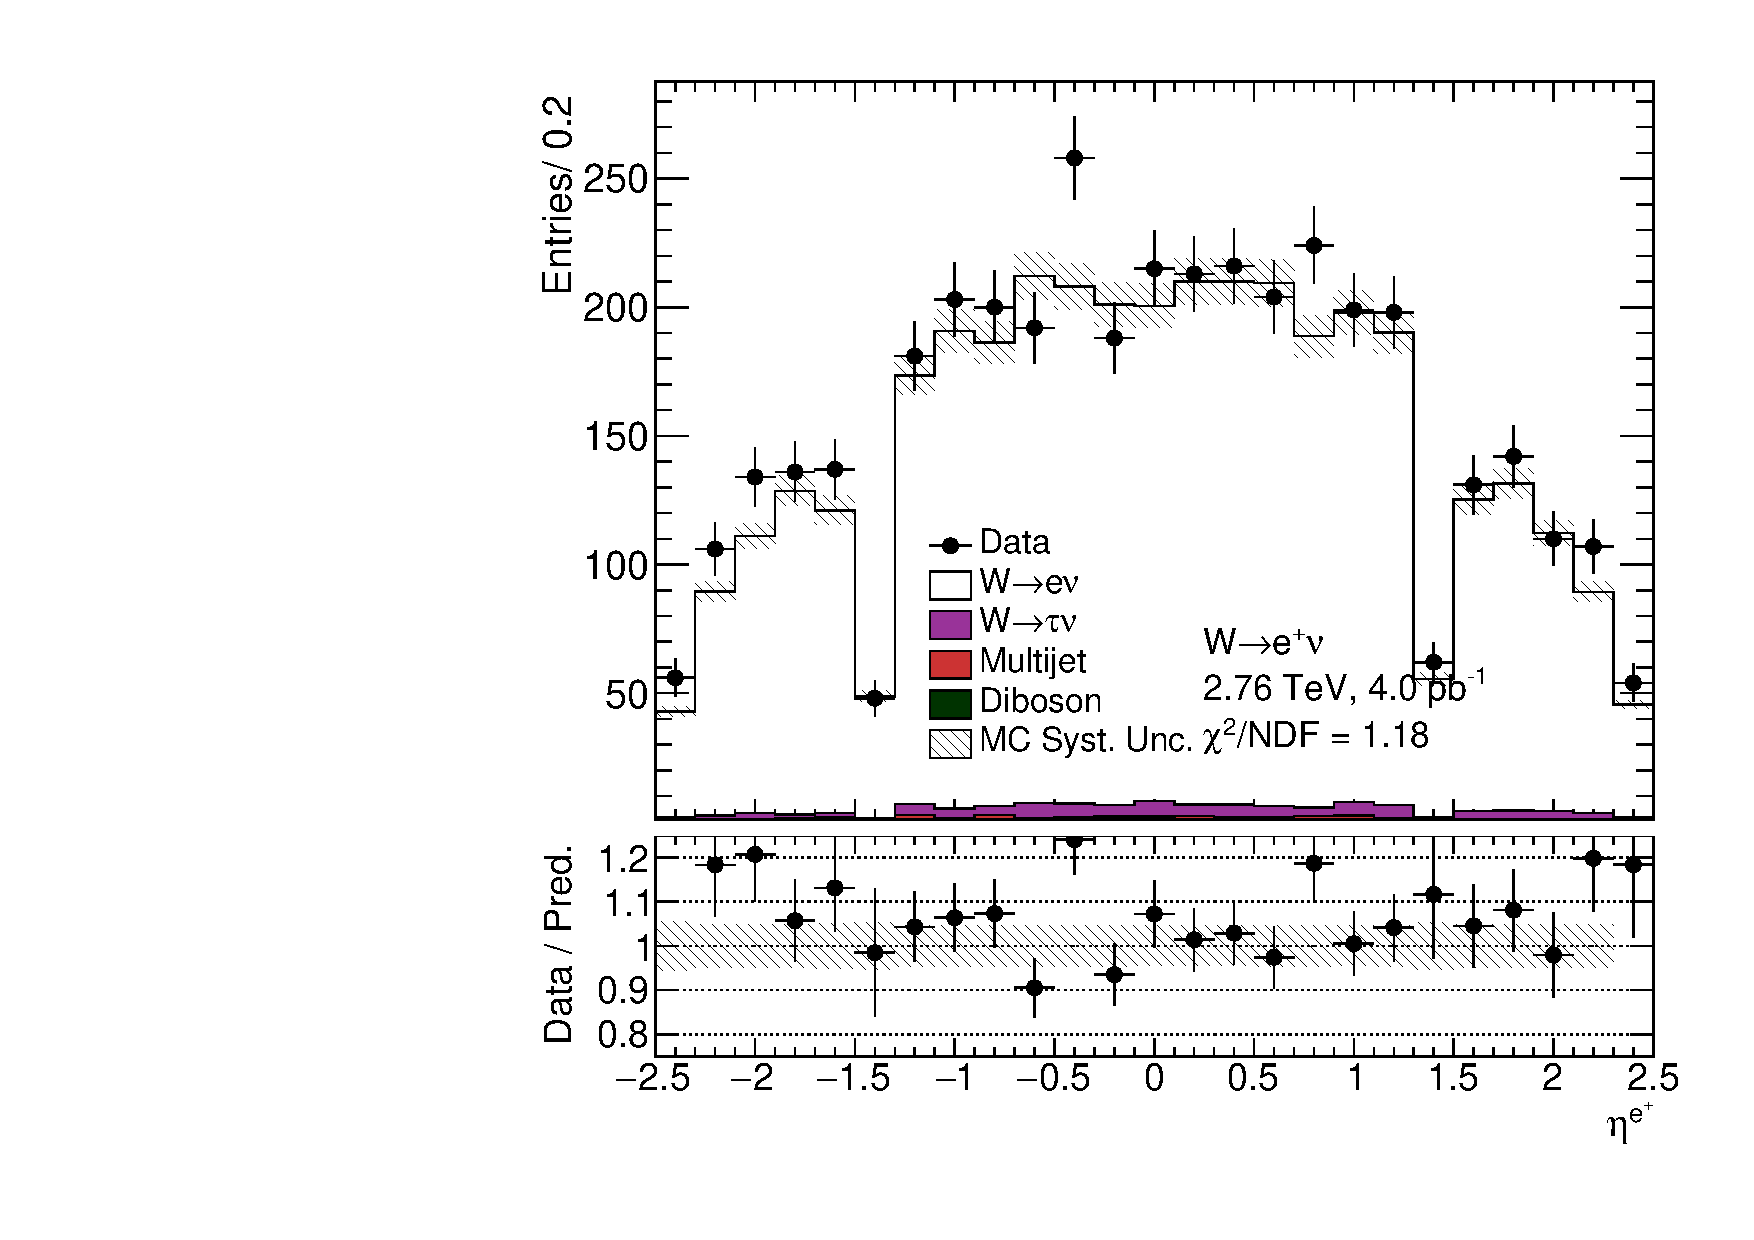
\includegraphics[width=1.\linewidth]{ControlPlots/Wanalysis/W_Plus_lepEta.pdf} \\ a)}
\end{minipage}
\hfill
\begin{minipage}[h]{0.49\linewidth}
\center{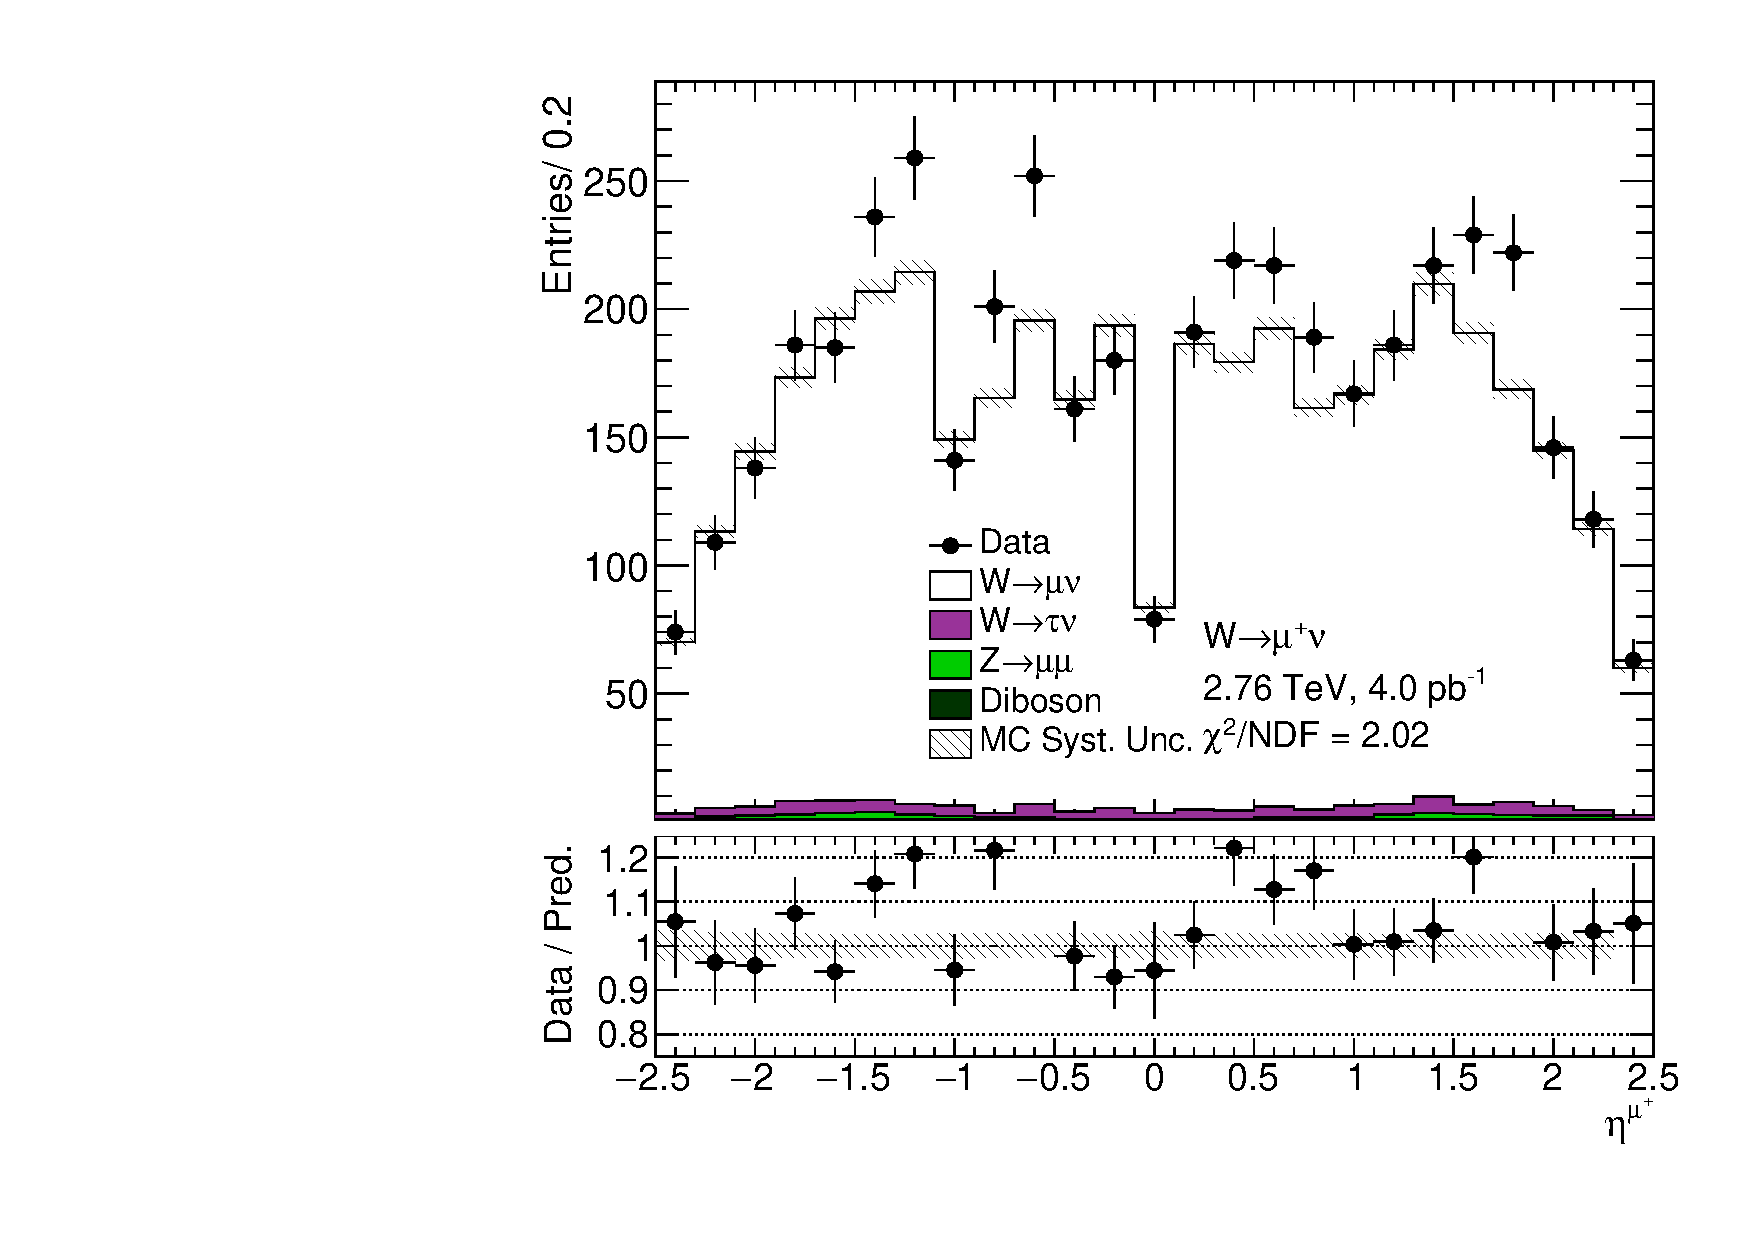
\includegraphics[width=1.\linewidth]{ControlPlots/Wanalysis/Wmu_Plus_lepEta.pdf} \\ b)}
\end{minipage}
\label{ris:WlnuPLep}
\caption{Lepton pseudorapidity distribution from the a) $W^{+} \to e^{+} \nu$ selection and  b) the $W^{+} \to \mu^{+} \nu$ selection.}
\end{figure}

\begin{figure}[h]
\begin{minipage}[h]{0.49\linewidth}
\center{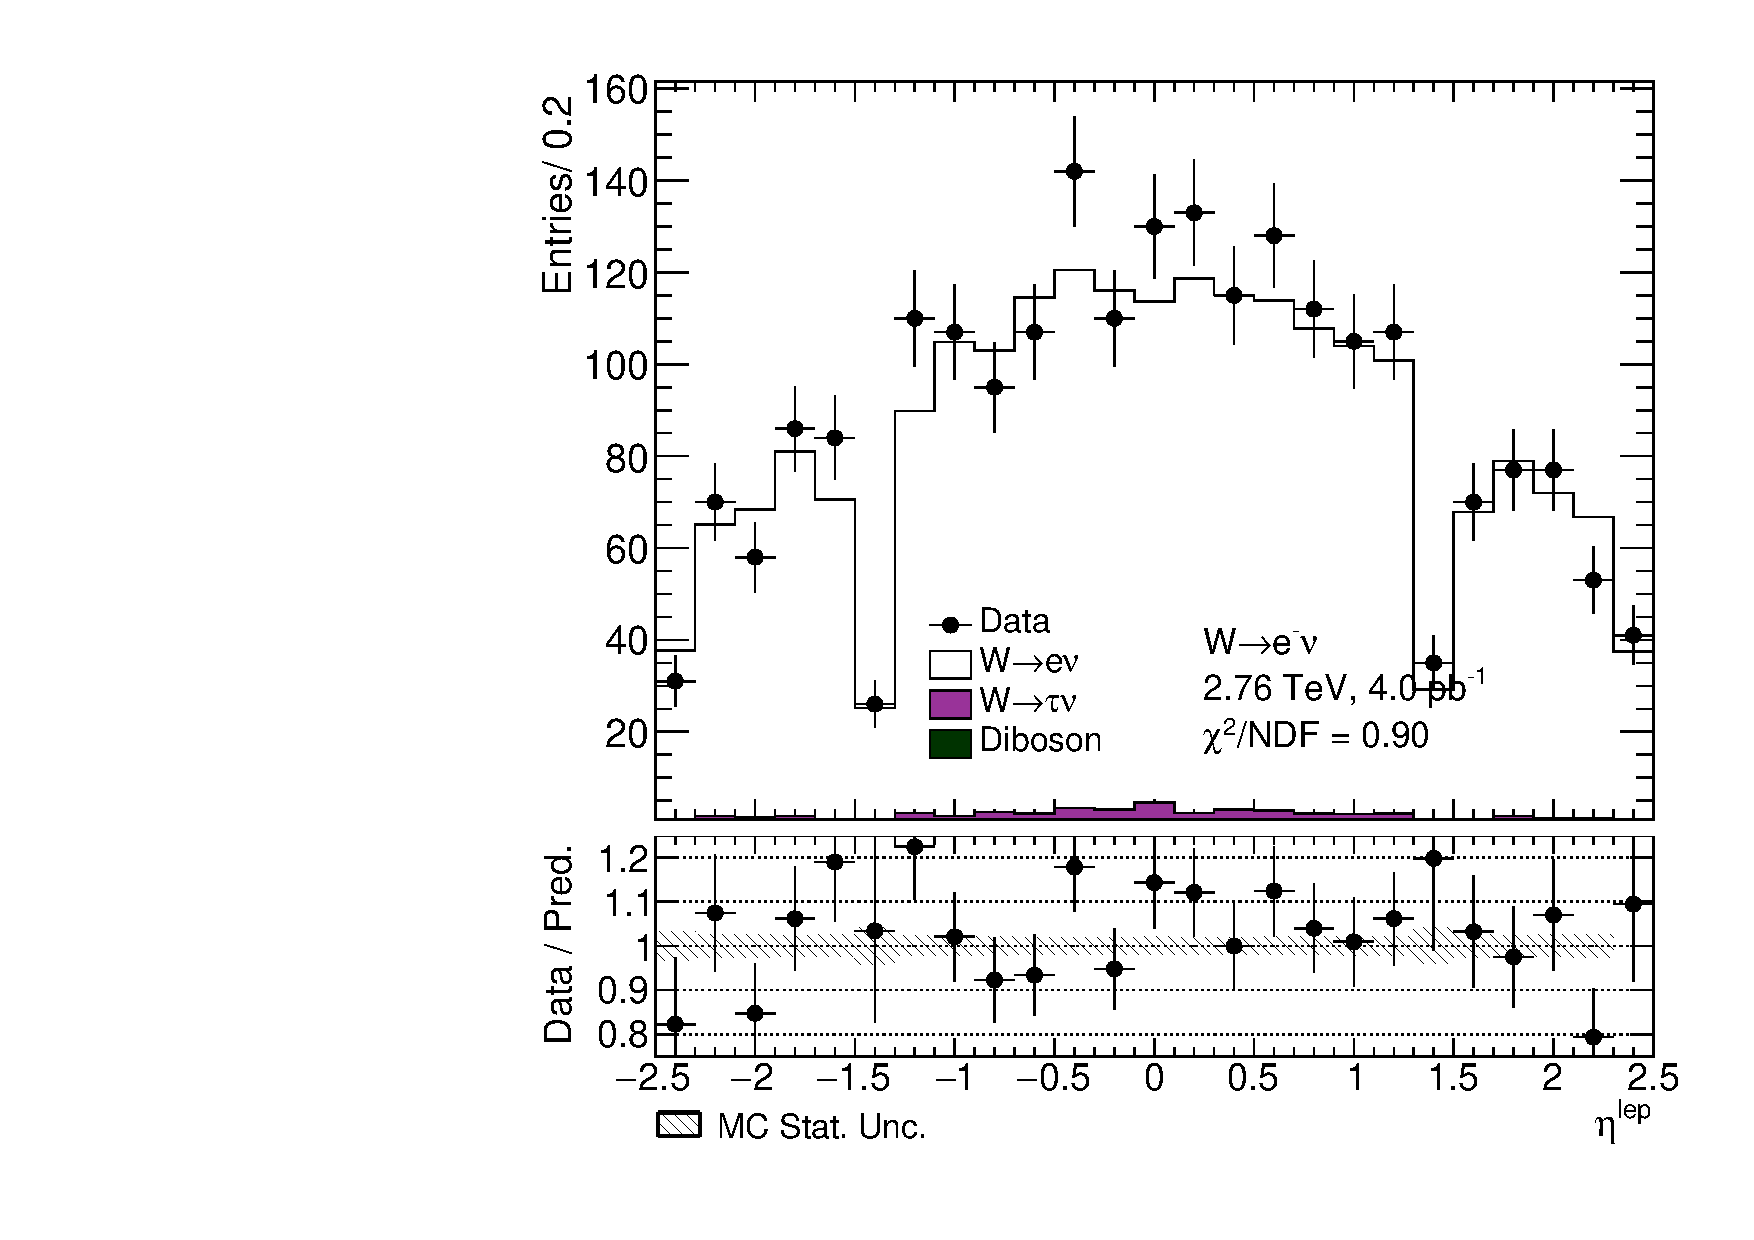
\includegraphics[width=1.\linewidth]{ControlPlots/Wanalysis/W_Minus_lepEta.pdf} \\ a)}
\end{minipage}
\hfill
\begin{minipage}[h]{0.49\linewidth}
\center{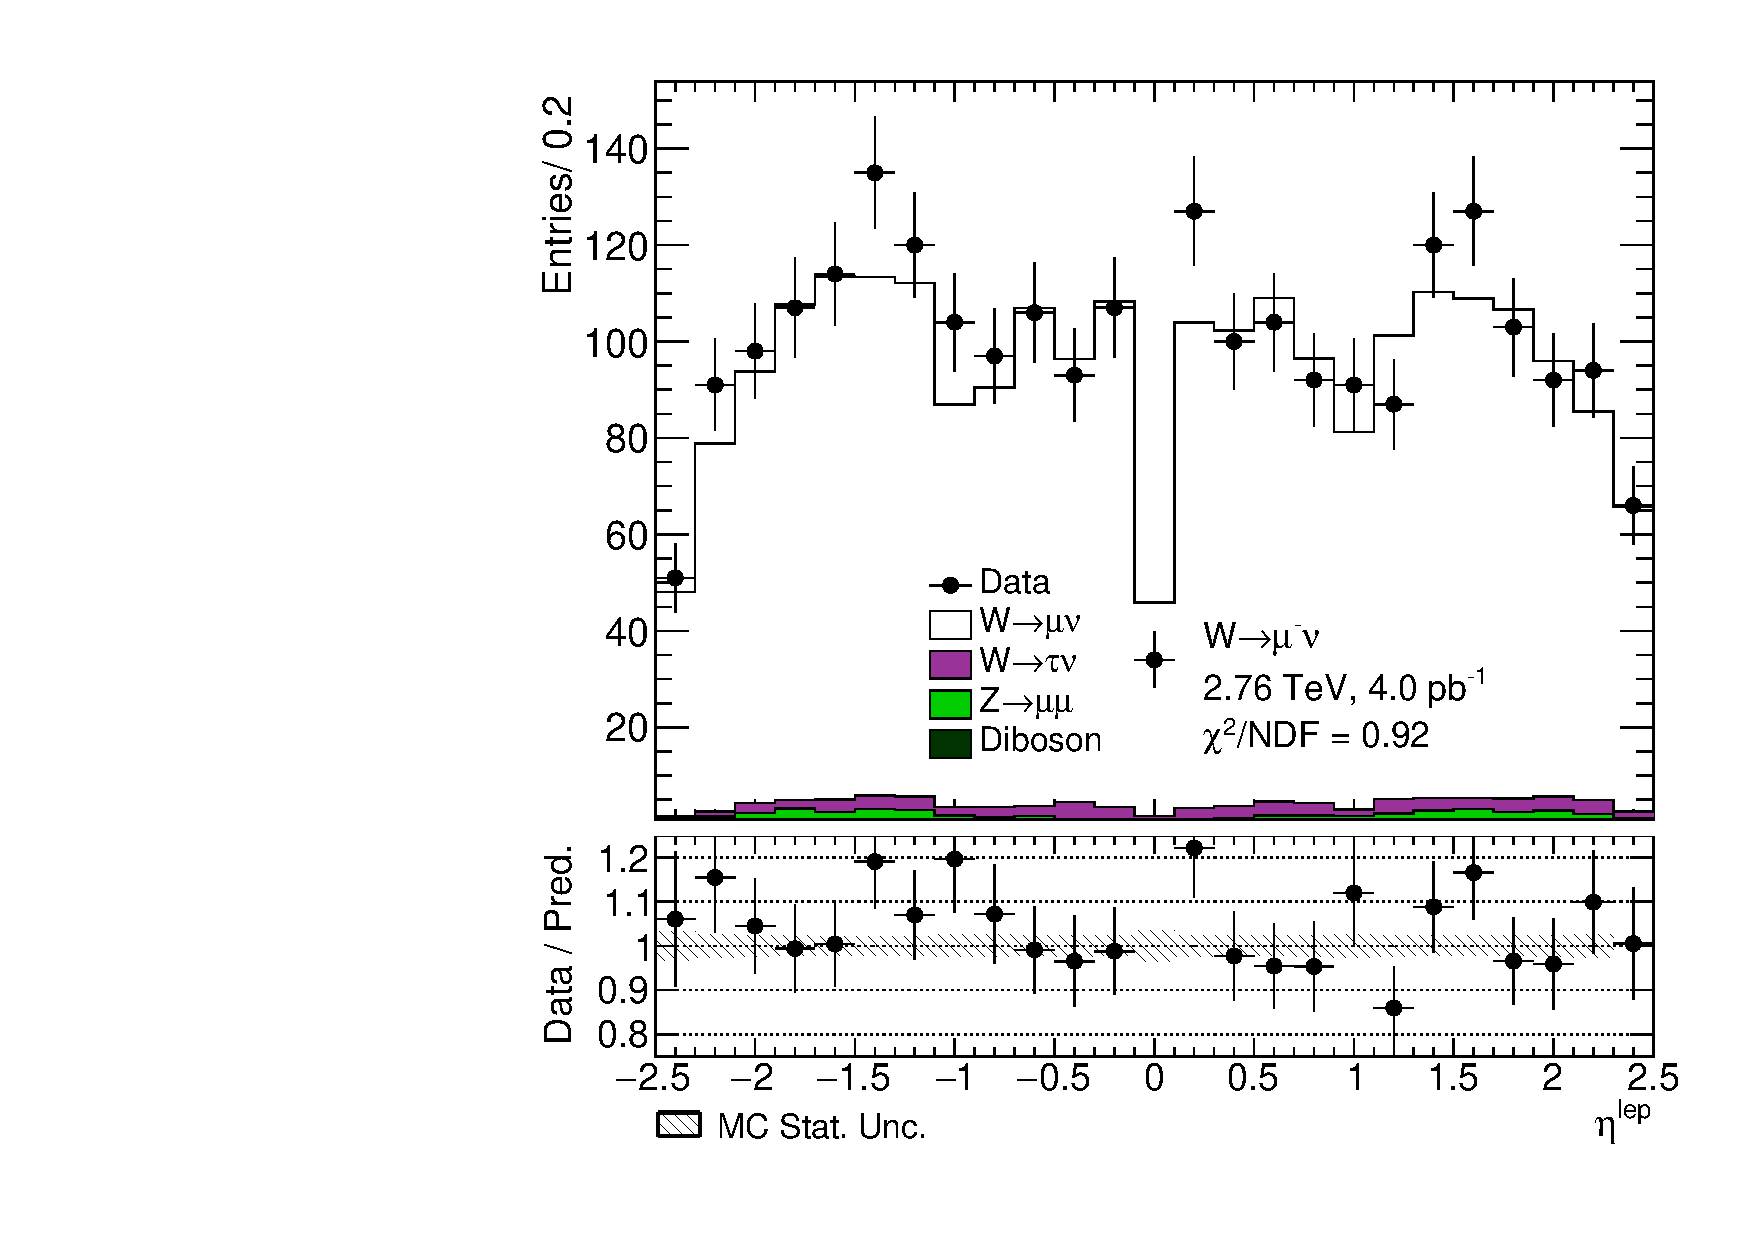
\includegraphics[width=1.\linewidth]{ControlPlots/Wanalysis/Wmu_Minus_lepEta.pdf} \\ b)}
\end{minipage}
\label{ris:WlnuMLep}
\caption{Lepton pseudorapidity distribution from the a) $W^{-} \to e^{-} \nu$ selection and  b) the $W^{-} \to \mu^{-} \nu$ selection.}
\end{figure}

%============================================================================================================
% Lep Pt

\begin{figure}[h]
\begin{minipage}[h]{0.49\linewidth}
\center{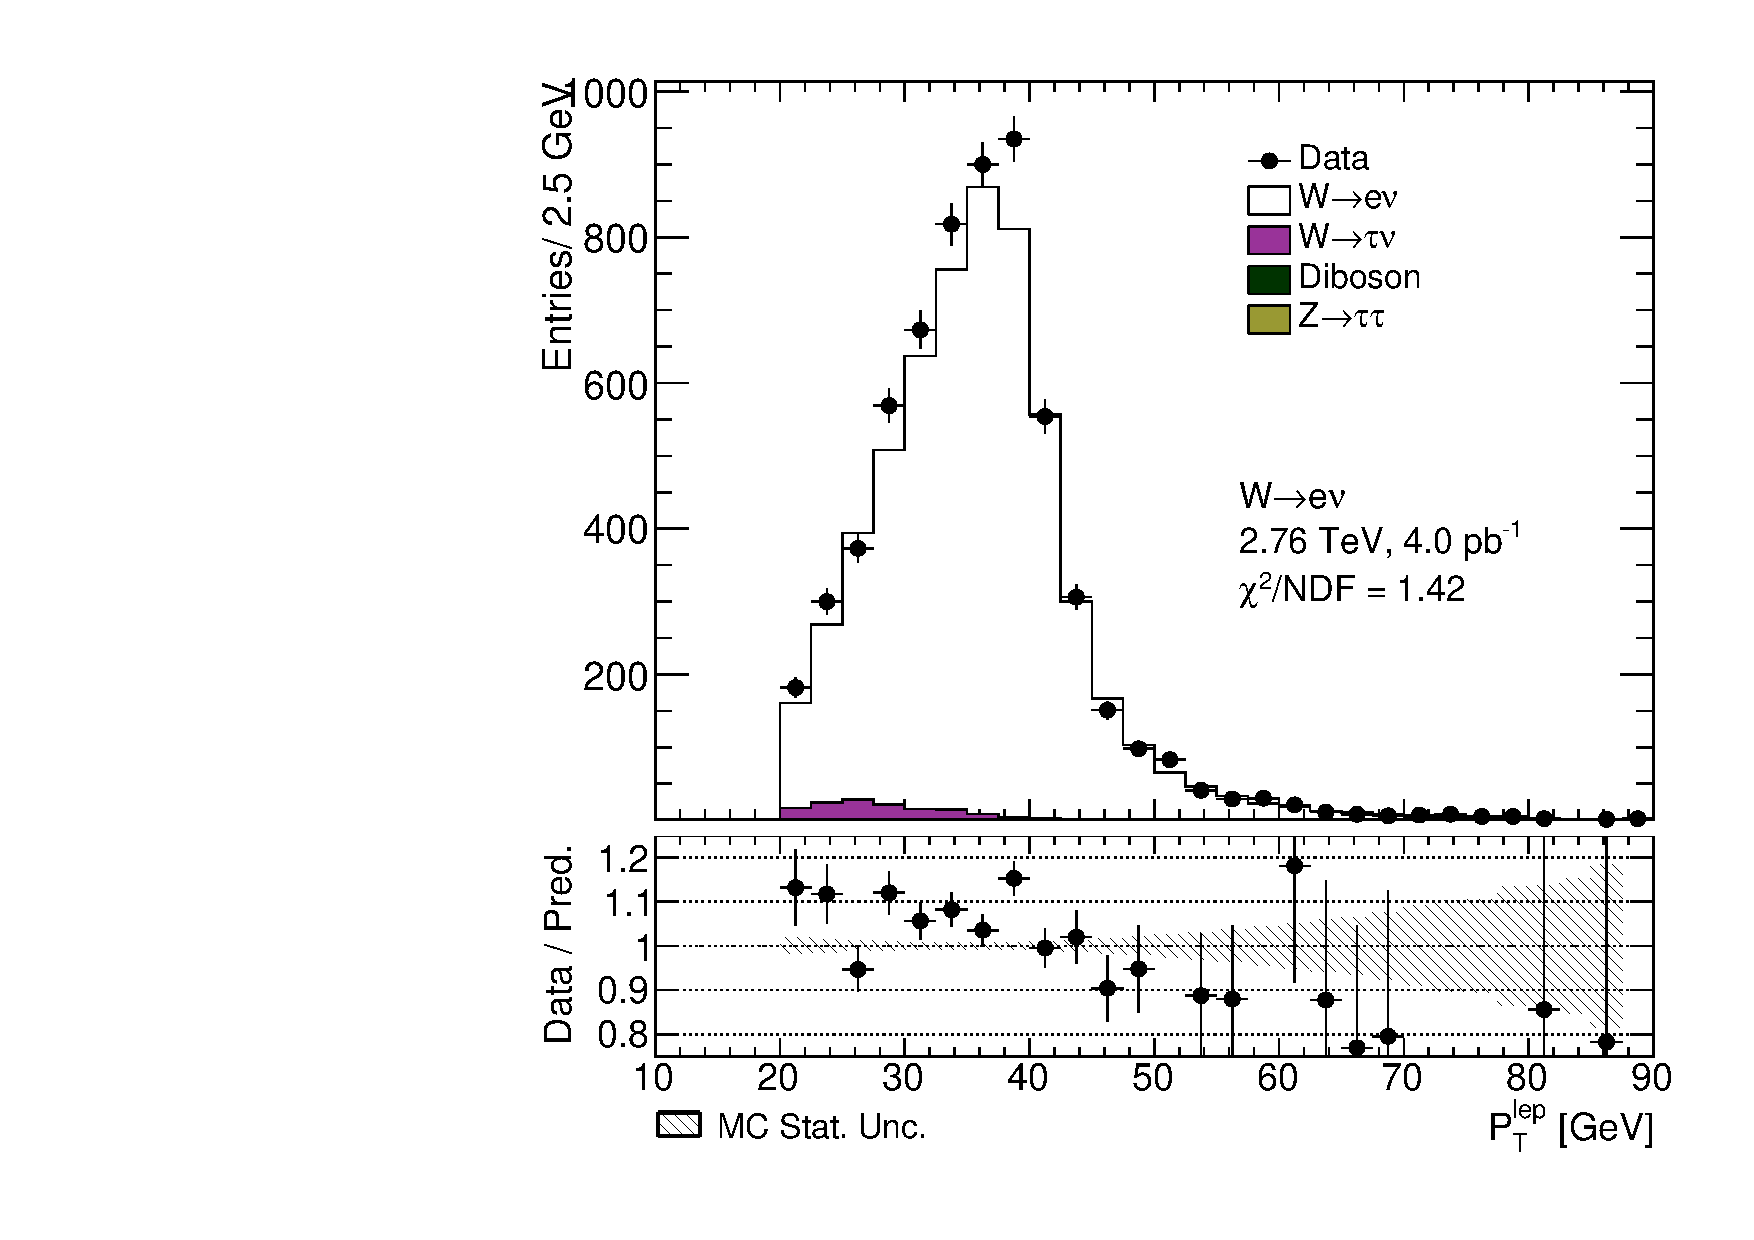
\includegraphics[width=1.\linewidth]{ControlPlots/Wanalysis/W_Boson_lepPt.pdf} \\ a)}
\end{minipage}
\hfill
\begin{minipage}[h]{0.49\linewidth}
\center{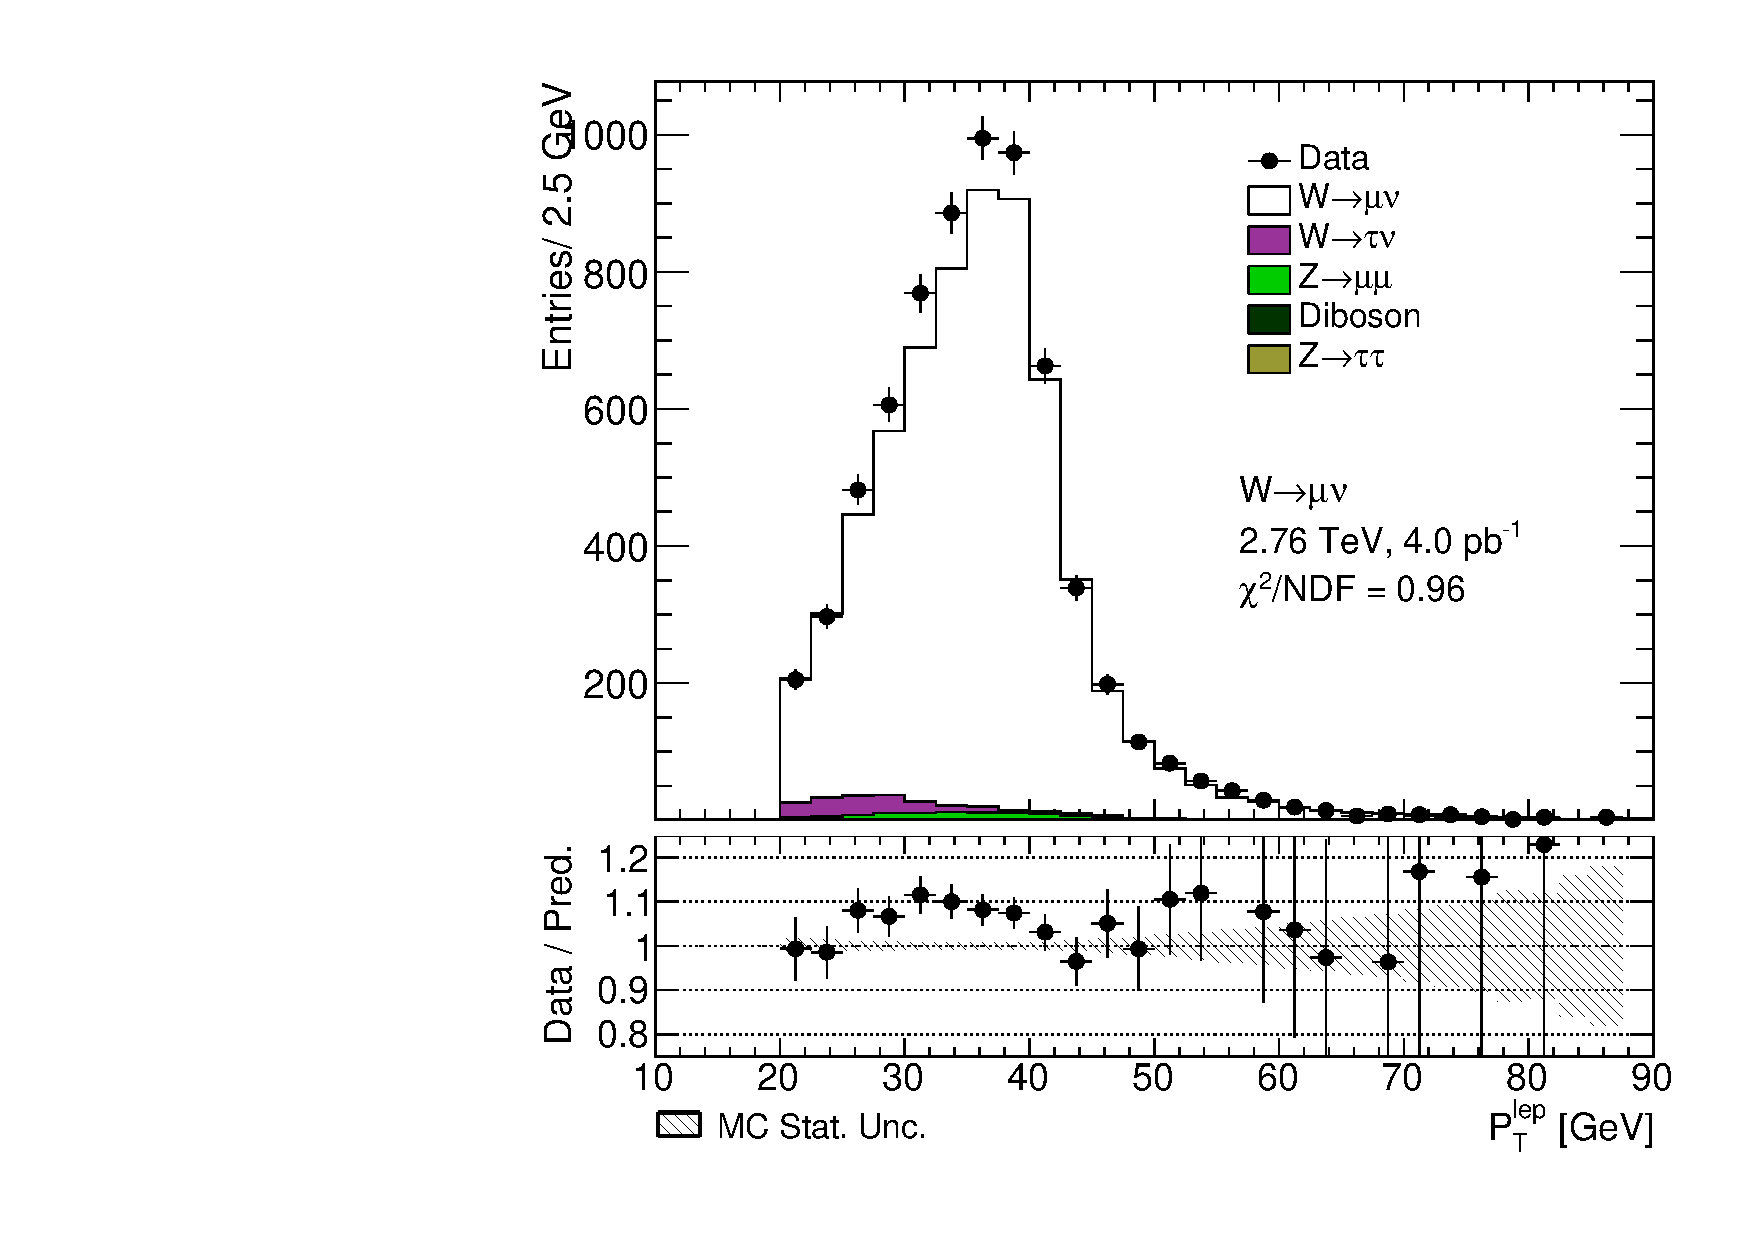
\includegraphics[width=1.\linewidth]{ControlPlots/Wanalysis/Wmu_Boson_lepPt.pdf} \\ b)}
\end{minipage}
\label{ris:WlnuLepPt}
\caption{Lepton transverse momentum distribution from the a) \wenu selection and  b) the \wmunu selection.}
\end{figure}

\begin{figure}[h]
\begin{minipage}[h]{0.49\linewidth}
\center{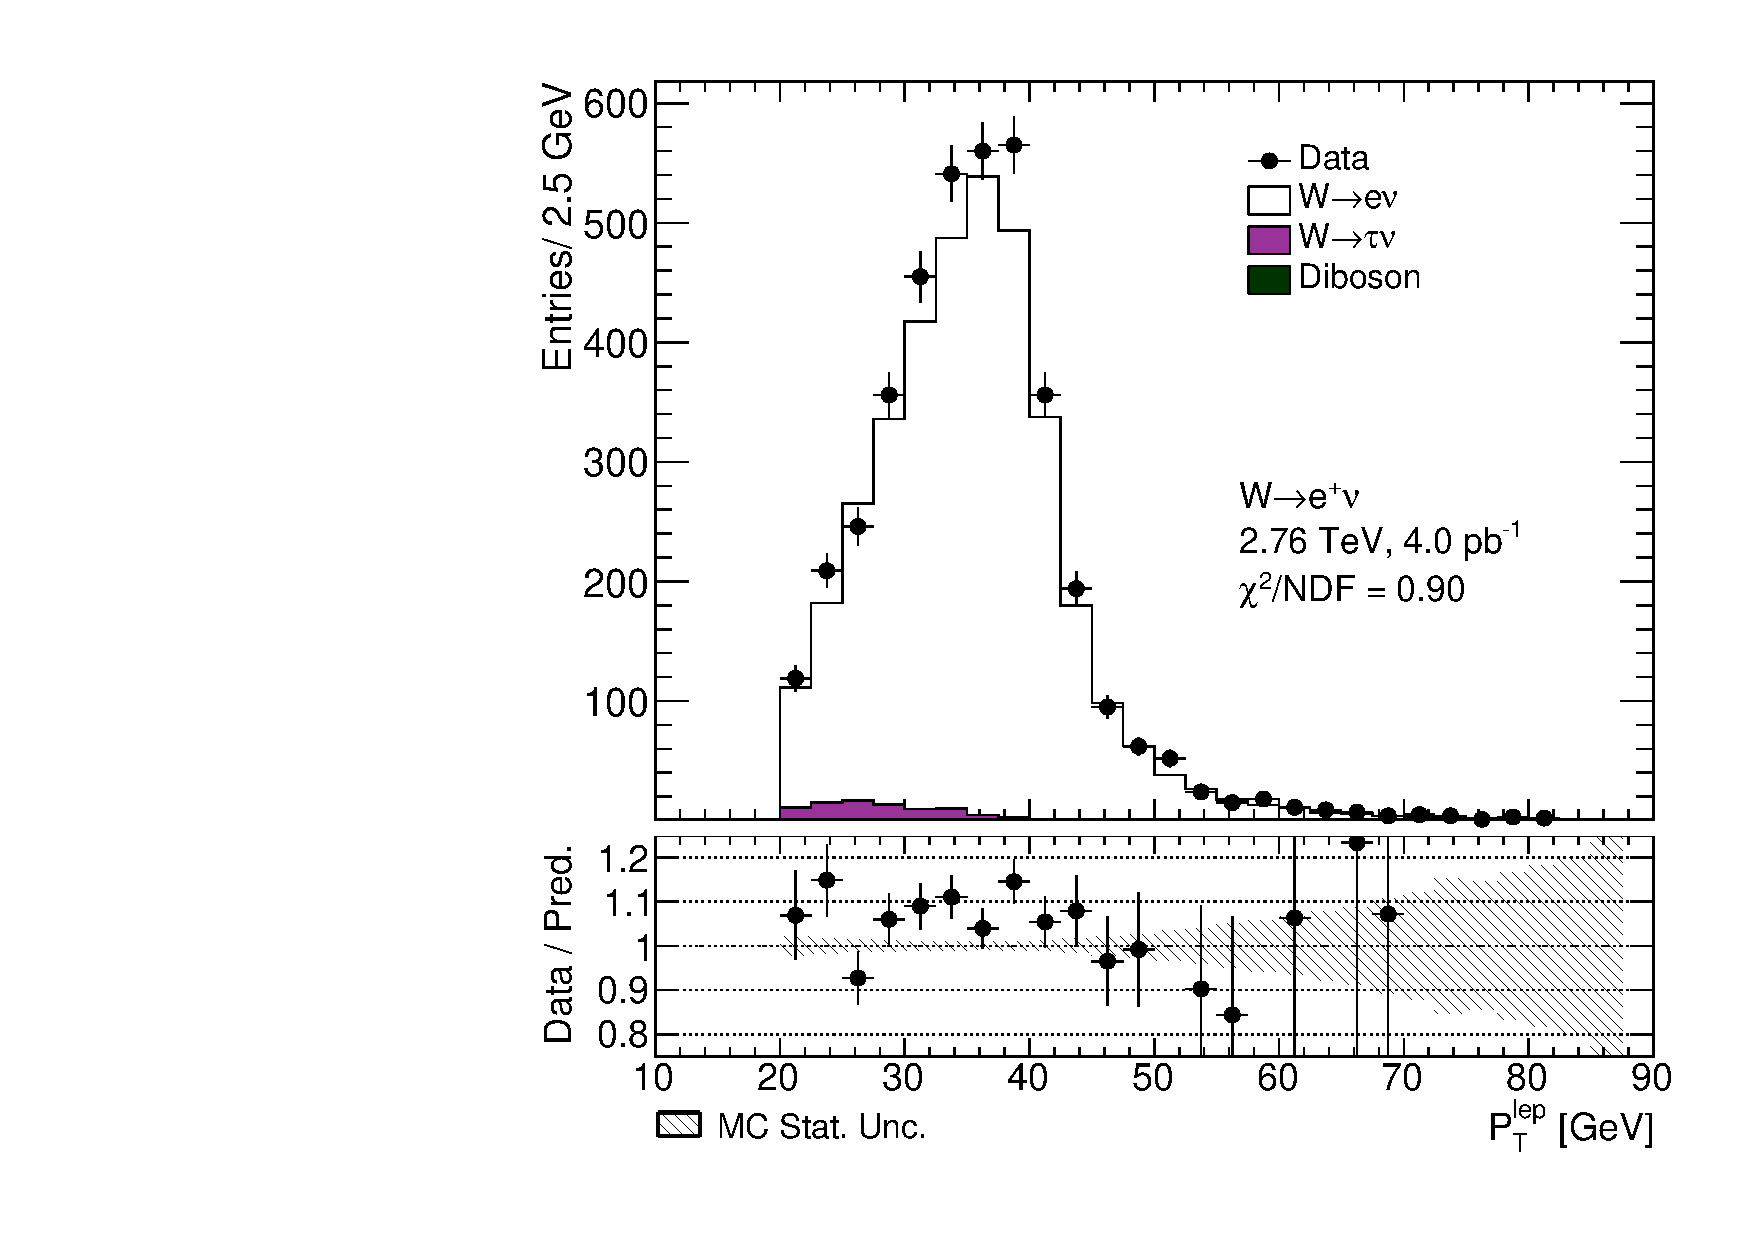
\includegraphics[width=1.\linewidth]{ControlPlots/Wanalysis/W_Plus_lepPt.pdf} \\ a)}
\end{minipage}
\hfill
\begin{minipage}[h]{0.49\linewidth}
\center{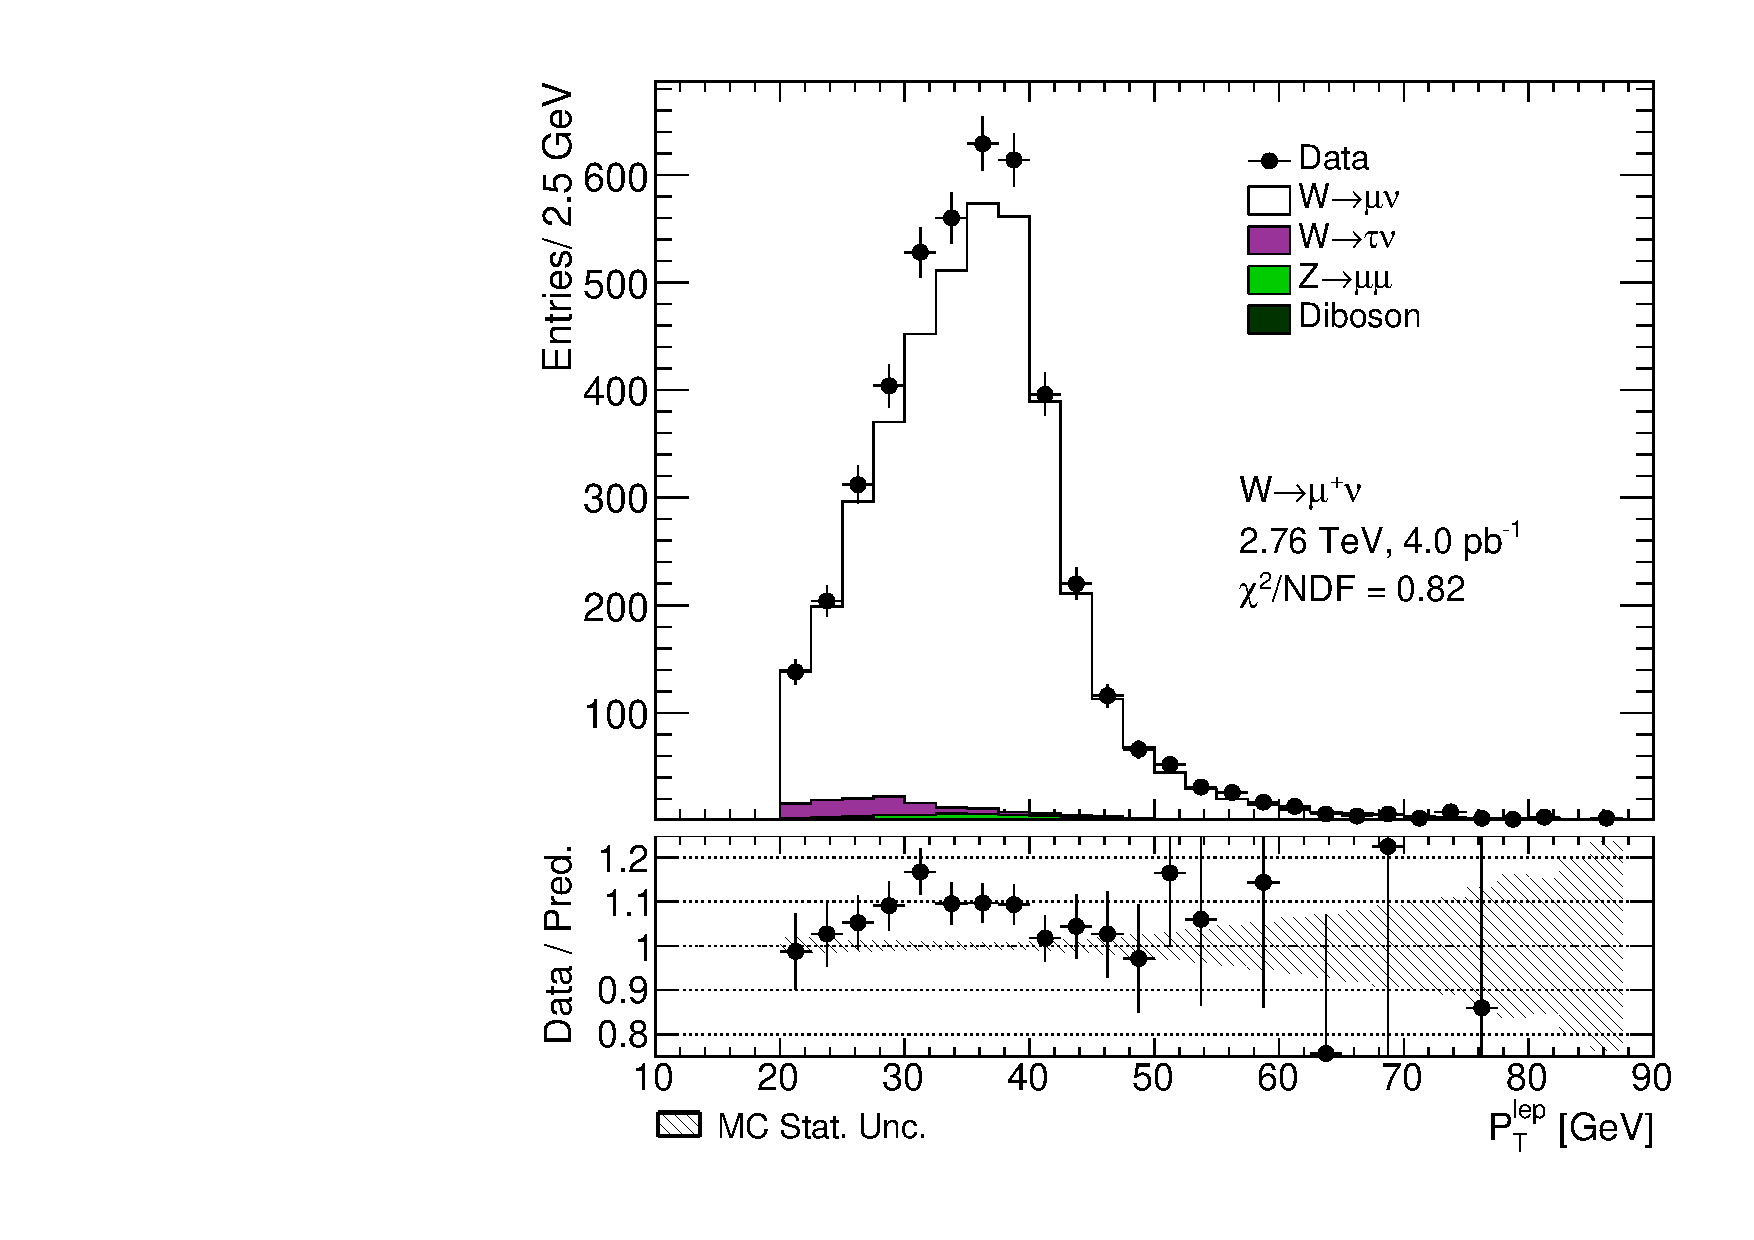
\includegraphics[width=1.\linewidth]{ControlPlots/Wanalysis/Wmu_Plus_lepPt.pdf} \\ b)}
\end{minipage}
\label{ris:WlnuPLepPt}
\caption{Lepton transverse momentum distribution from the a) $W^{+} \to e^{+} \nu$ selection and  b) the $W^{+} \to \mu^{+} \nu$ selection.}
\end{figure}

\begin{figure}[h]
\begin{minipage}[h]{0.49\linewidth}
\center{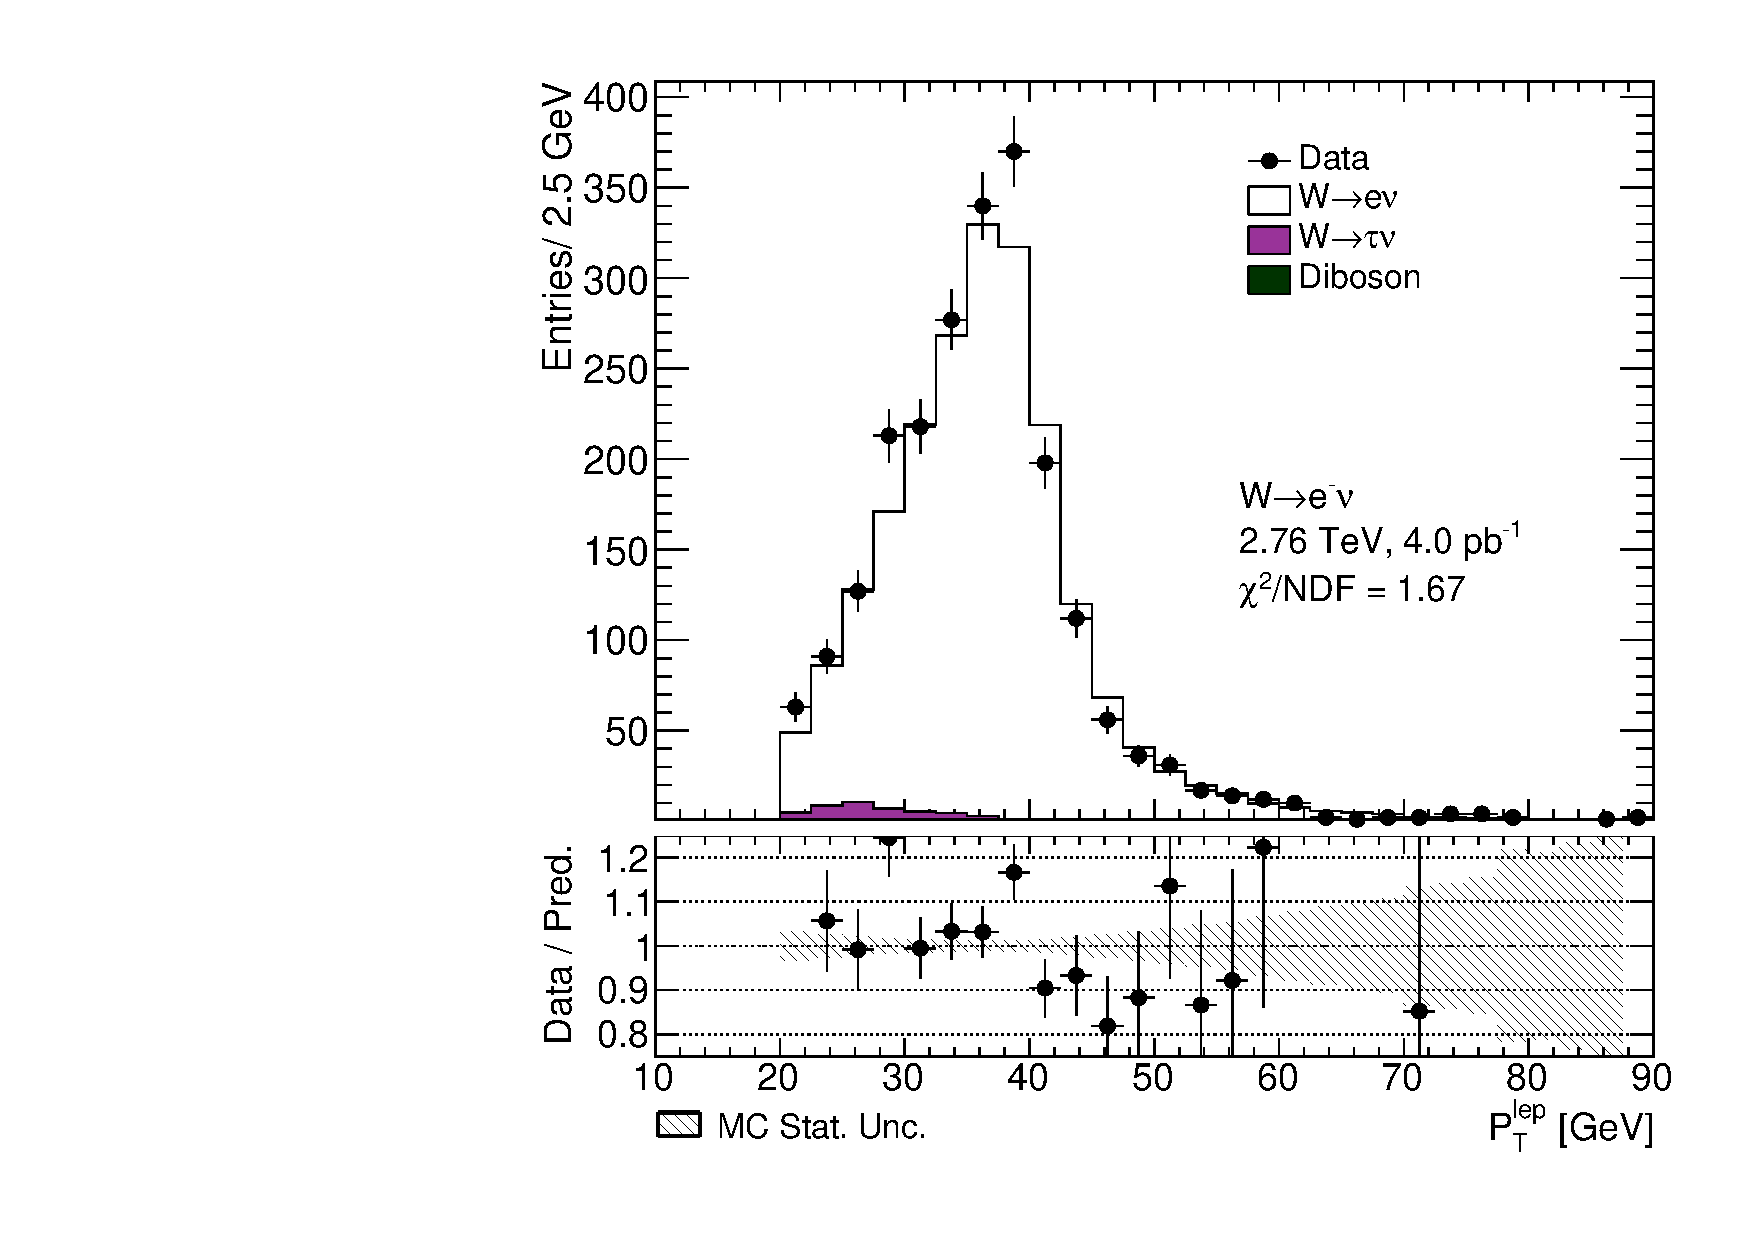
\includegraphics[width=1.\linewidth]{ControlPlots/Wanalysis/W_Minus_lepPt.pdf} \\ a)}
\end{minipage}
\hfill
\begin{minipage}[h]{0.49\linewidth}
\center{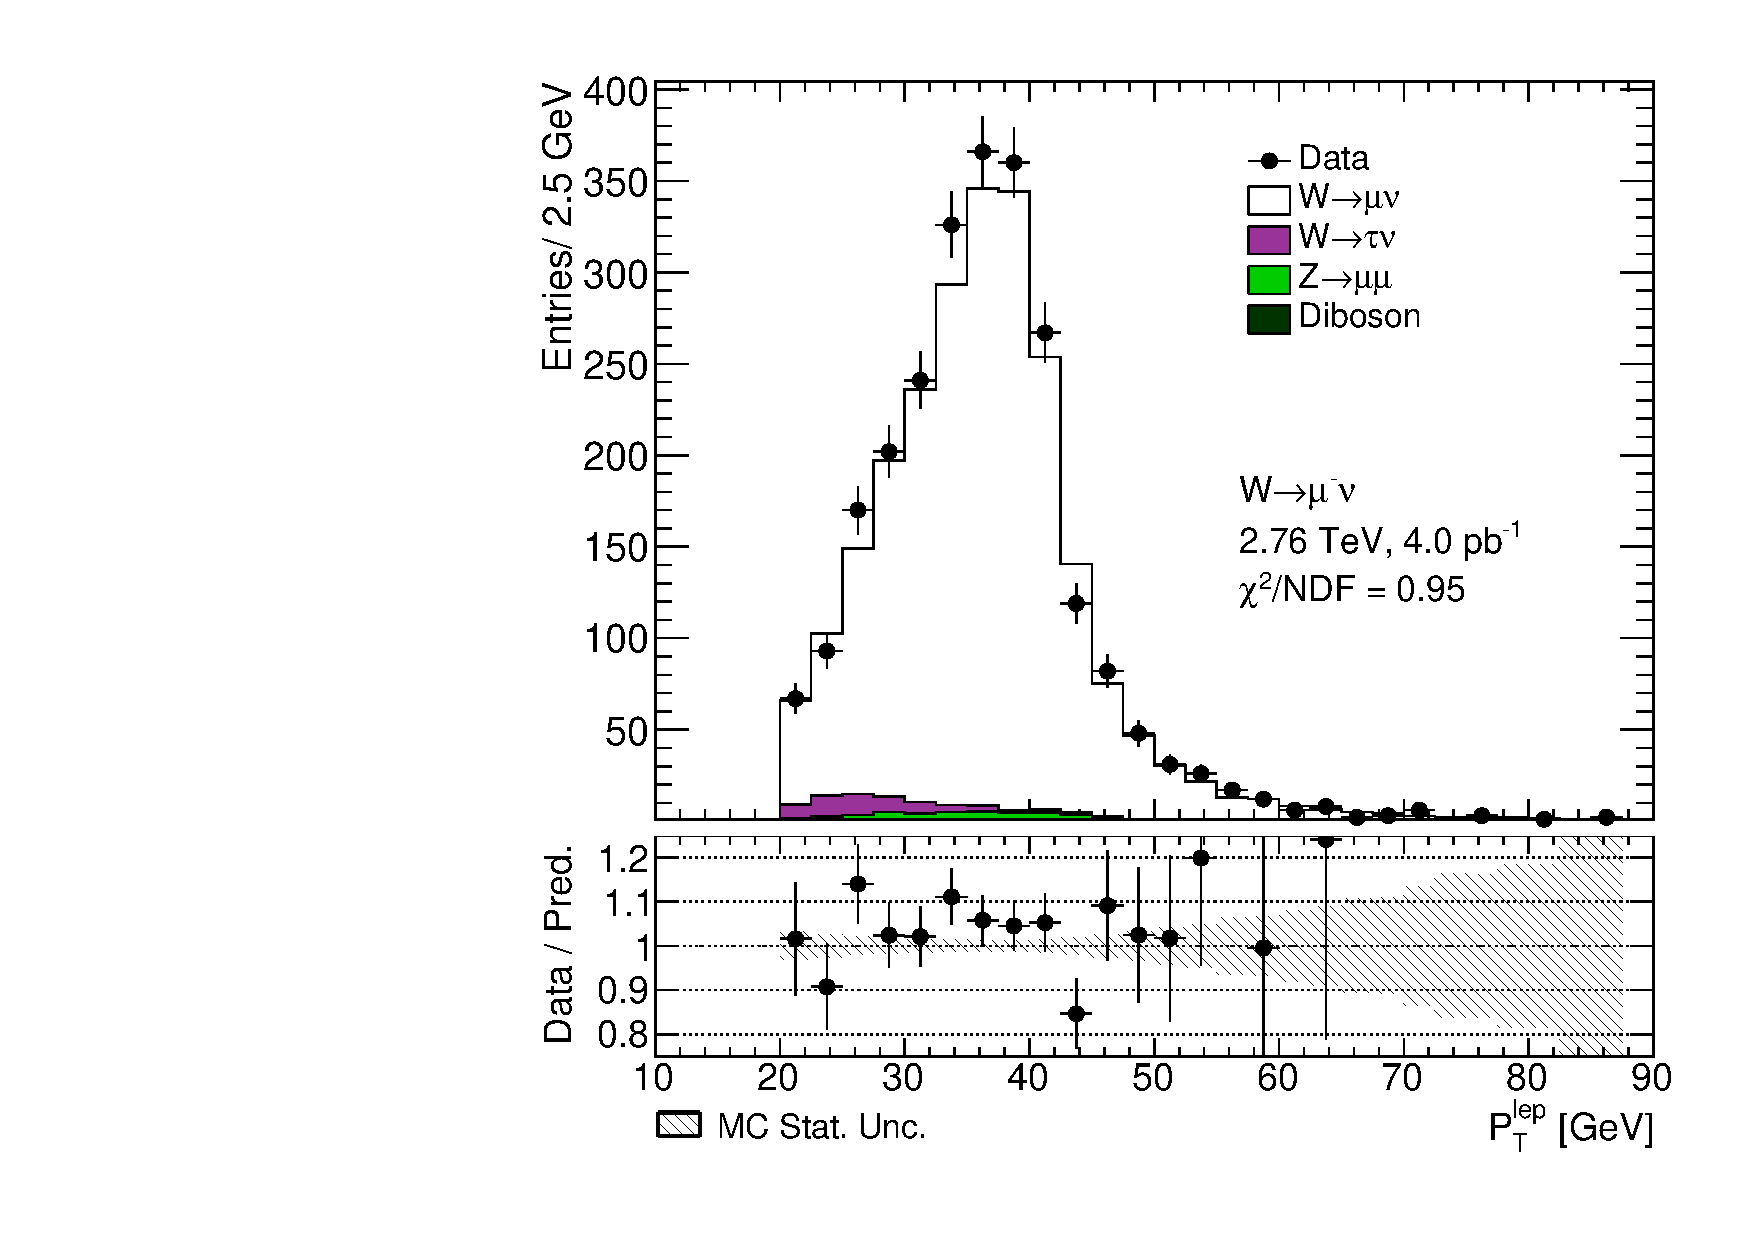
\includegraphics[width=1.\linewidth]{ControlPlots/Wanalysis/Wmu_Minus_lepPt.pdf} \\ b)}
\end{minipage}
\label{ris:WlnuMLepPt}
\caption{Lepton transverse momentum distribution from the a) $W^{-} \to e^{-} \nu$ selection and  b) the $W^{-} \to \mu^{-} \nu$ selection.}
\end{figure}


%============================================================================================================
% EtMiss


\begin{figure}[h]
\begin{minipage}[h]{0.49\linewidth}
\center{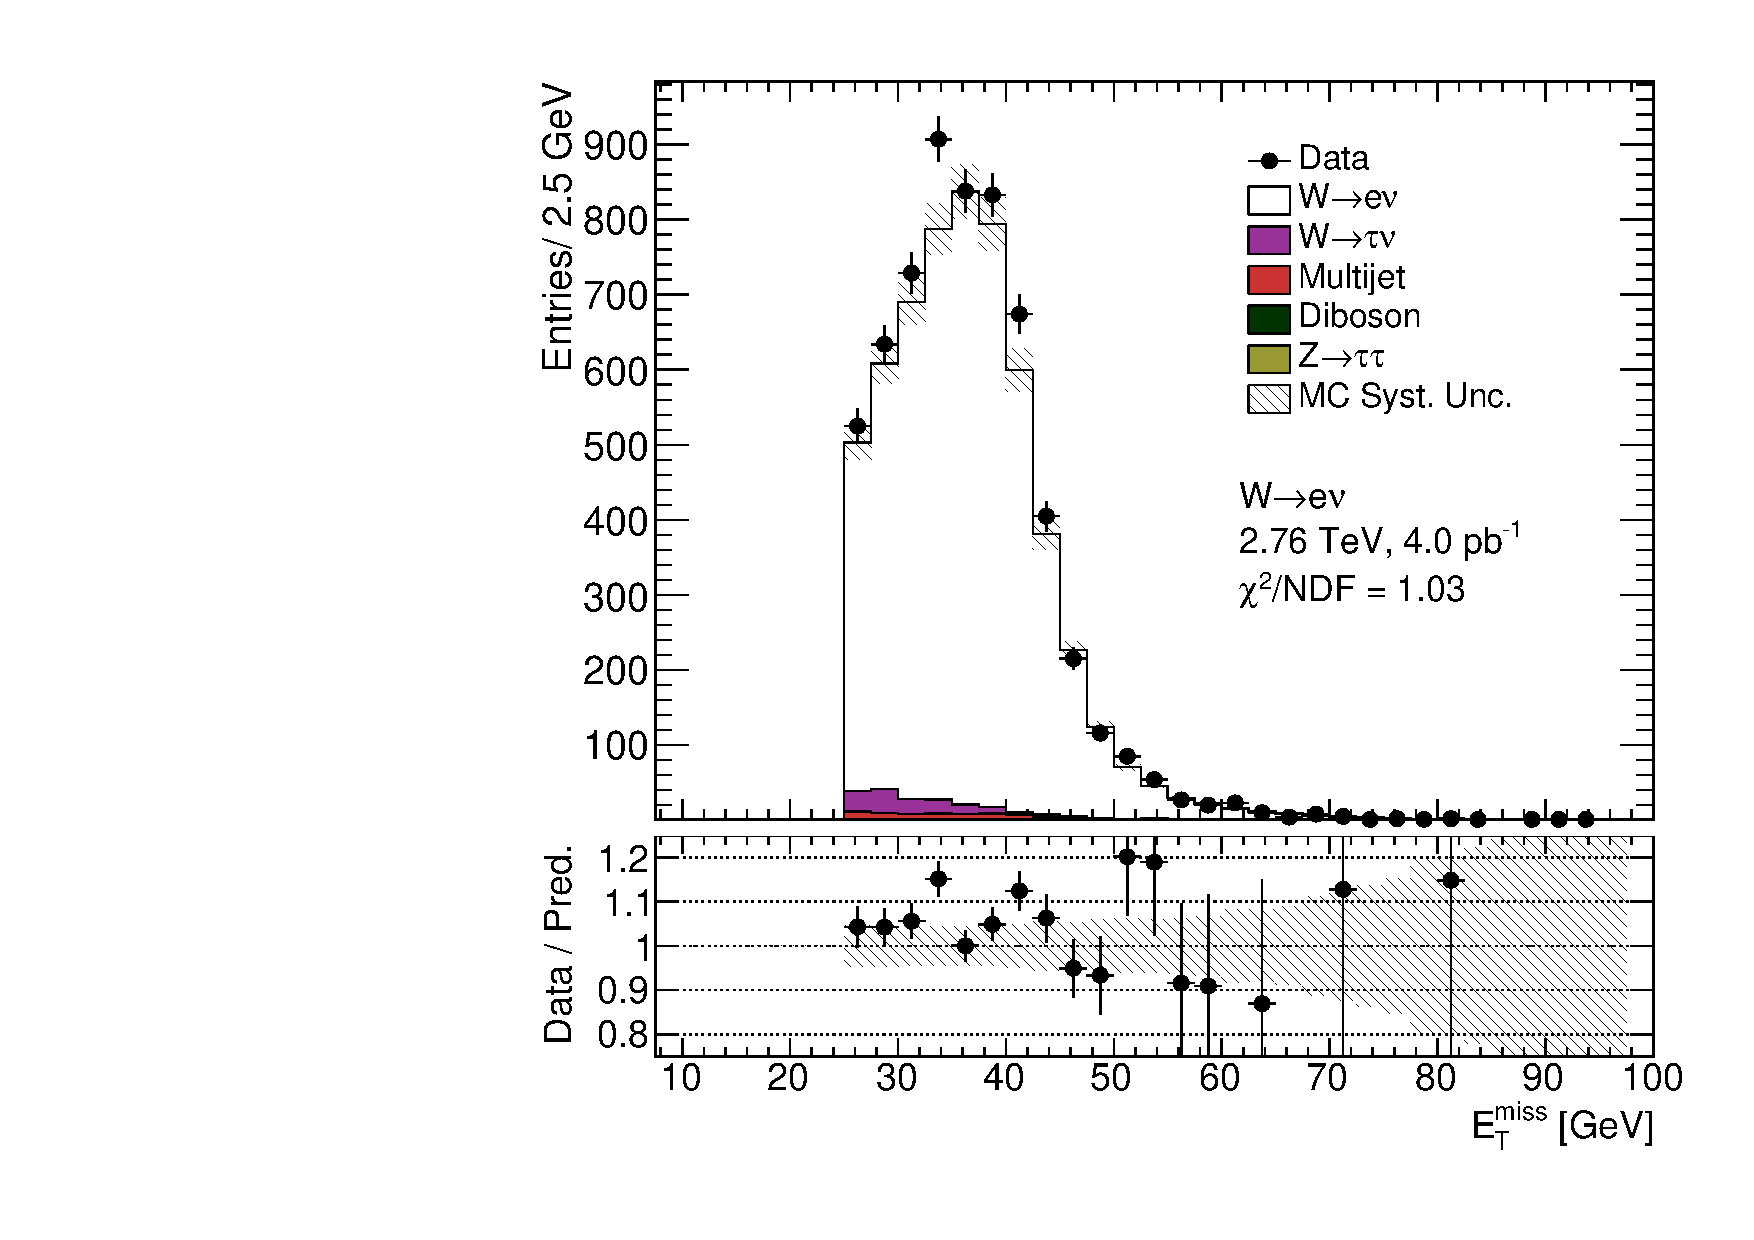
\includegraphics[width=1.\linewidth]{ControlPlots/Wanalysis/W_Boson_etMiss.pdf} \\ a)}
\end{minipage}
\hfill
\begin{minipage}[h]{0.49\linewidth}
\center{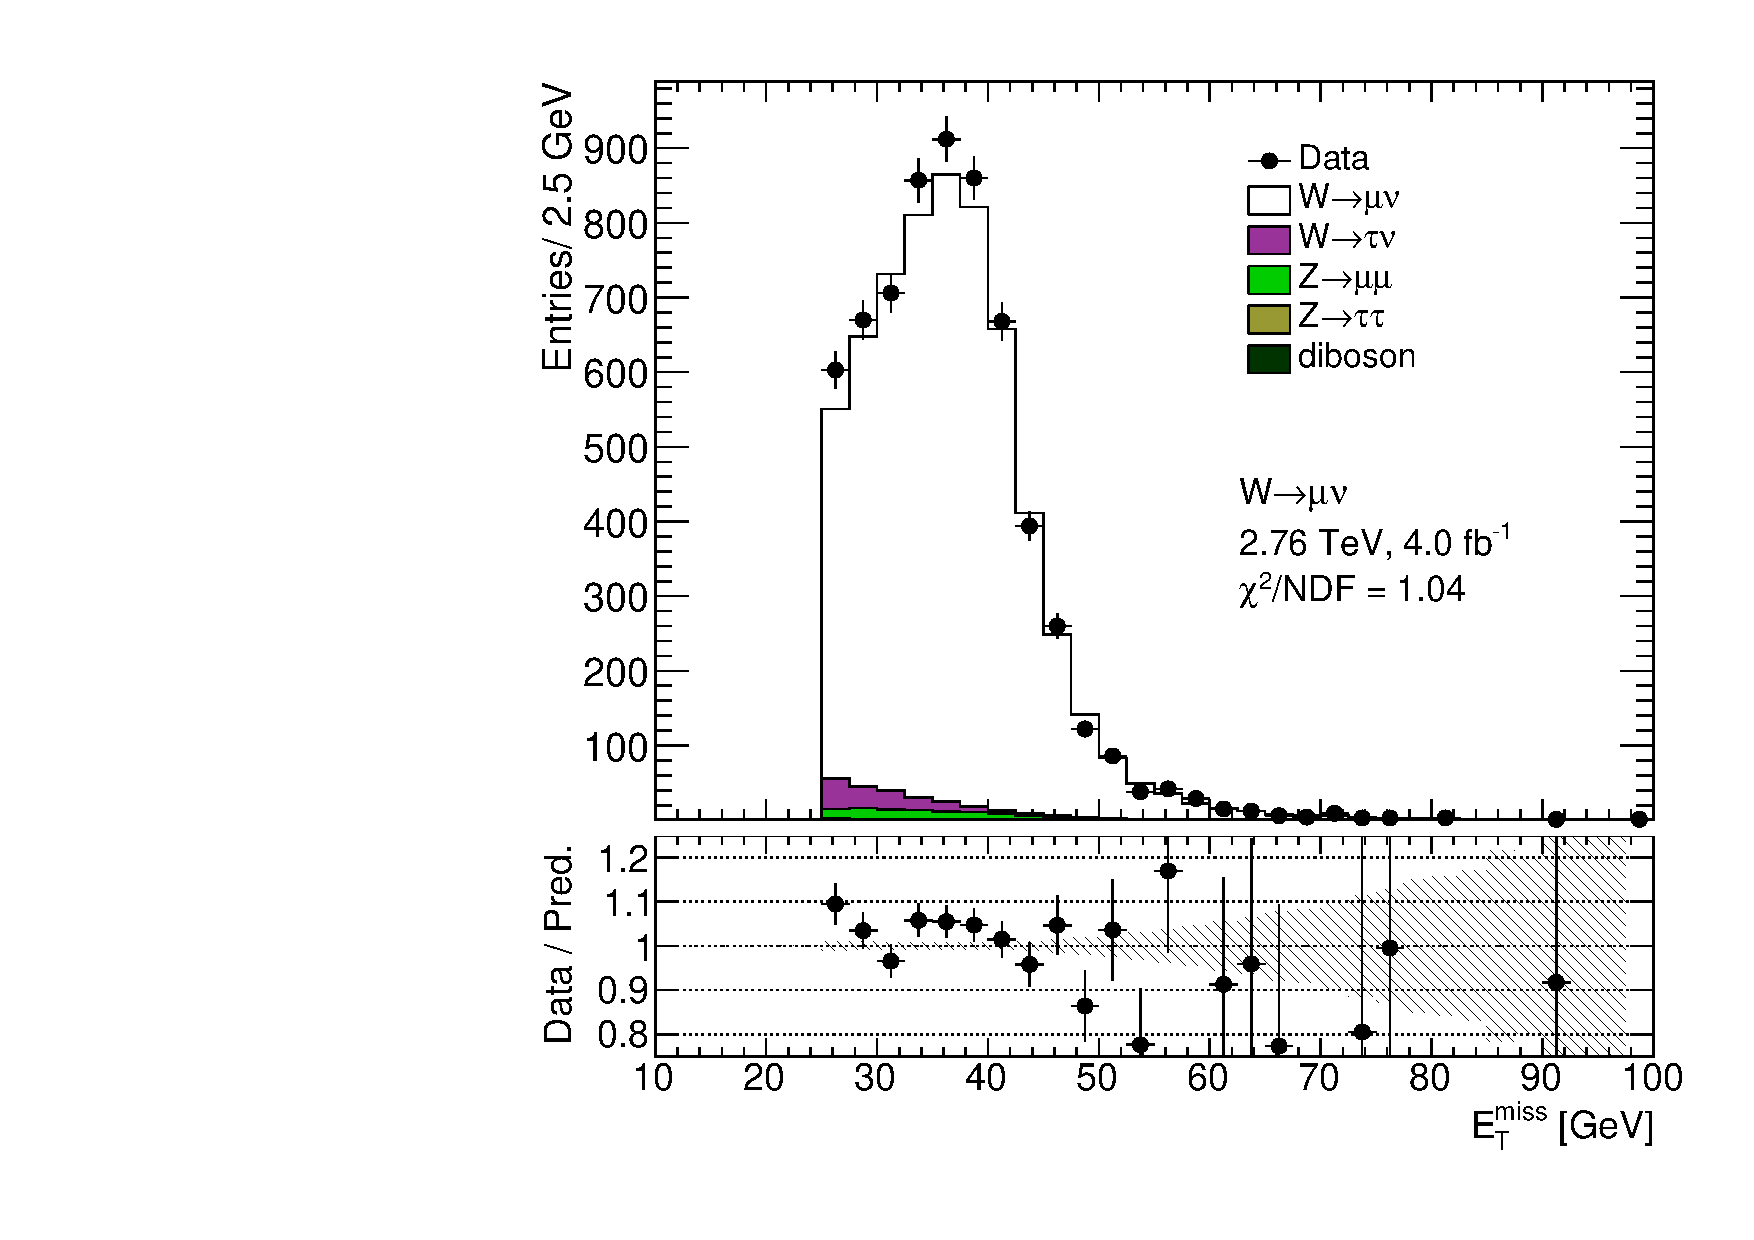
\includegraphics[width=1.\linewidth]{ControlPlots/Wanalysis/Wmu_Boson_etMiss.pdf} \\ b)}
\end{minipage}

\caption{Missing transverse energy distribution from the a) \wenu selection and  b) the \wmunu selection.}
\end{figure}

\begin{figure}[h]
\begin{minipage}[h]{0.49\linewidth}
\center{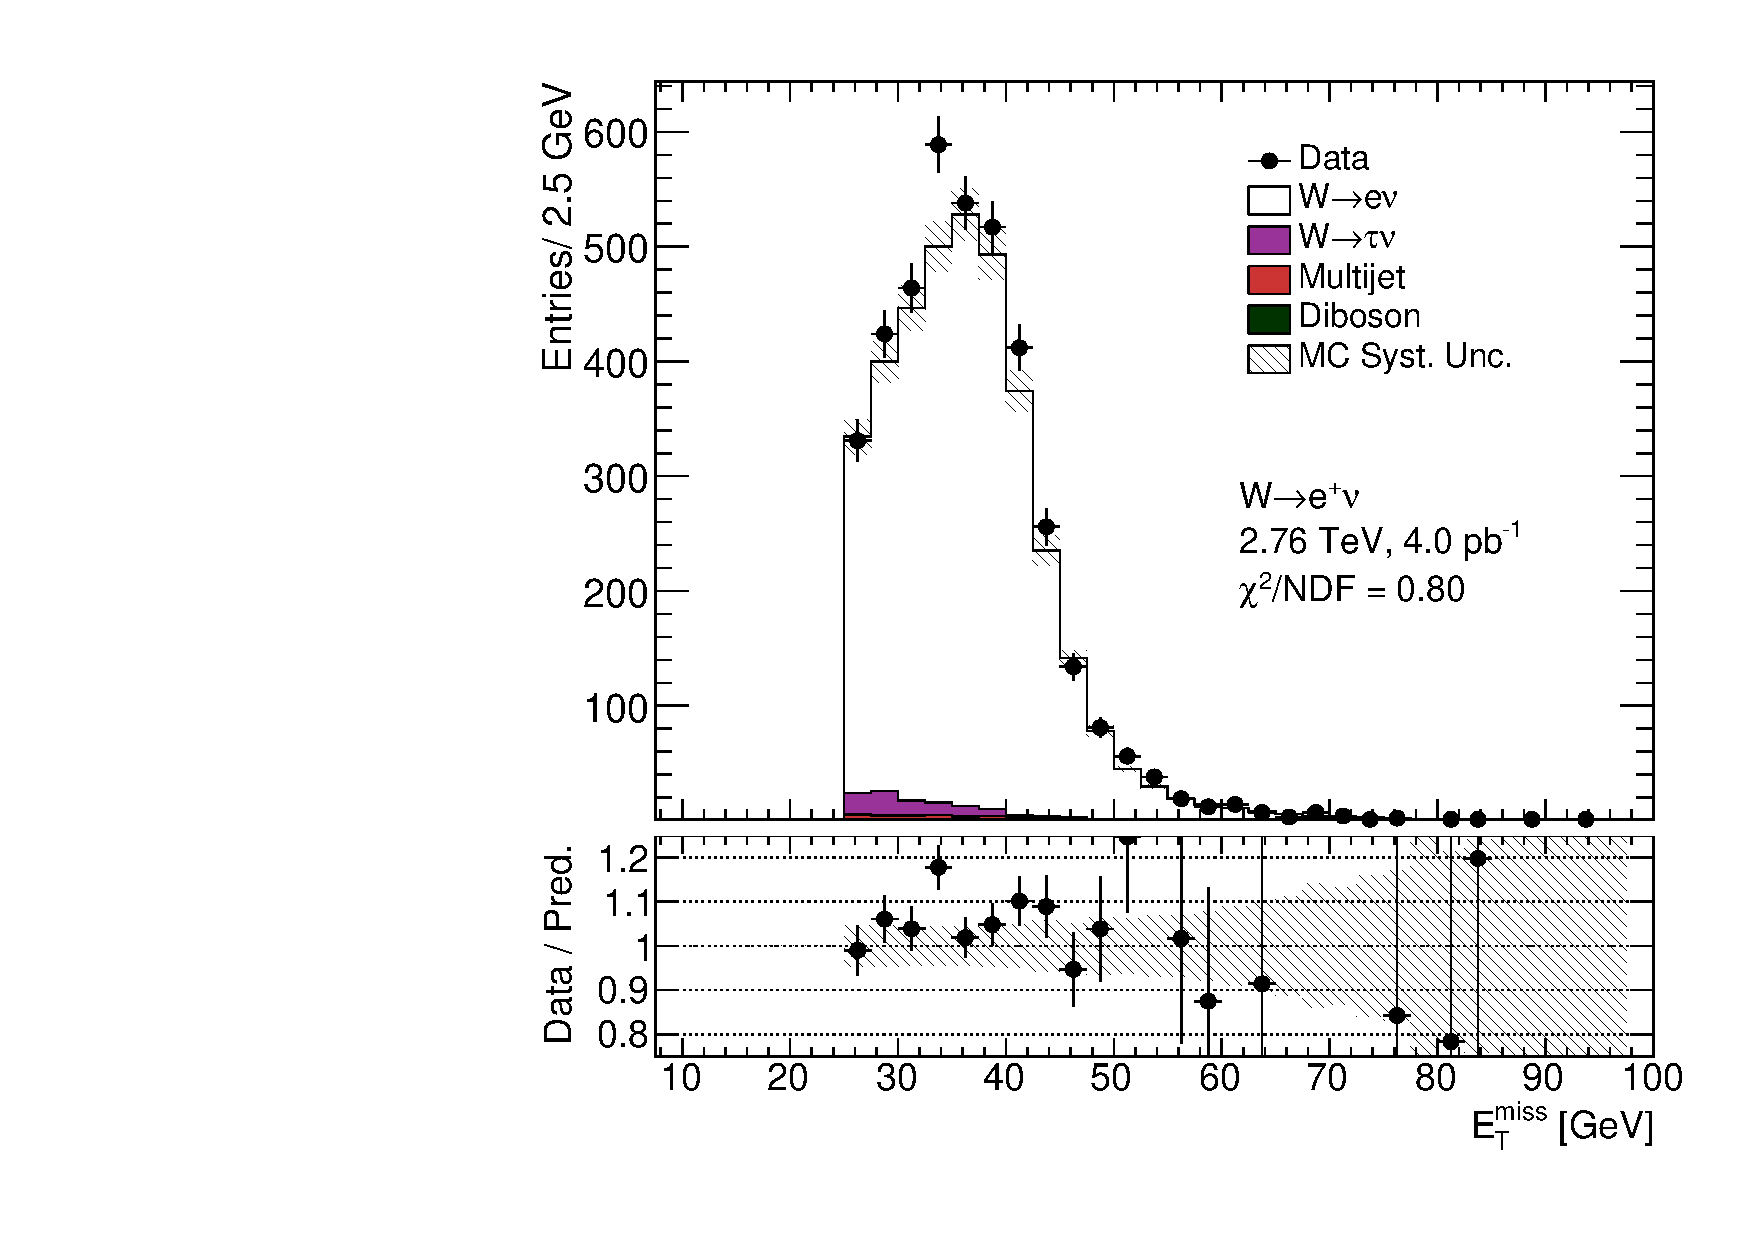
\includegraphics[width=1.\linewidth]{ControlPlots/Wanalysis/W_Plus_etMiss.pdf} \\ a)}
\end{minipage}
\hfill
\begin{minipage}[h]{0.49\linewidth}
\center{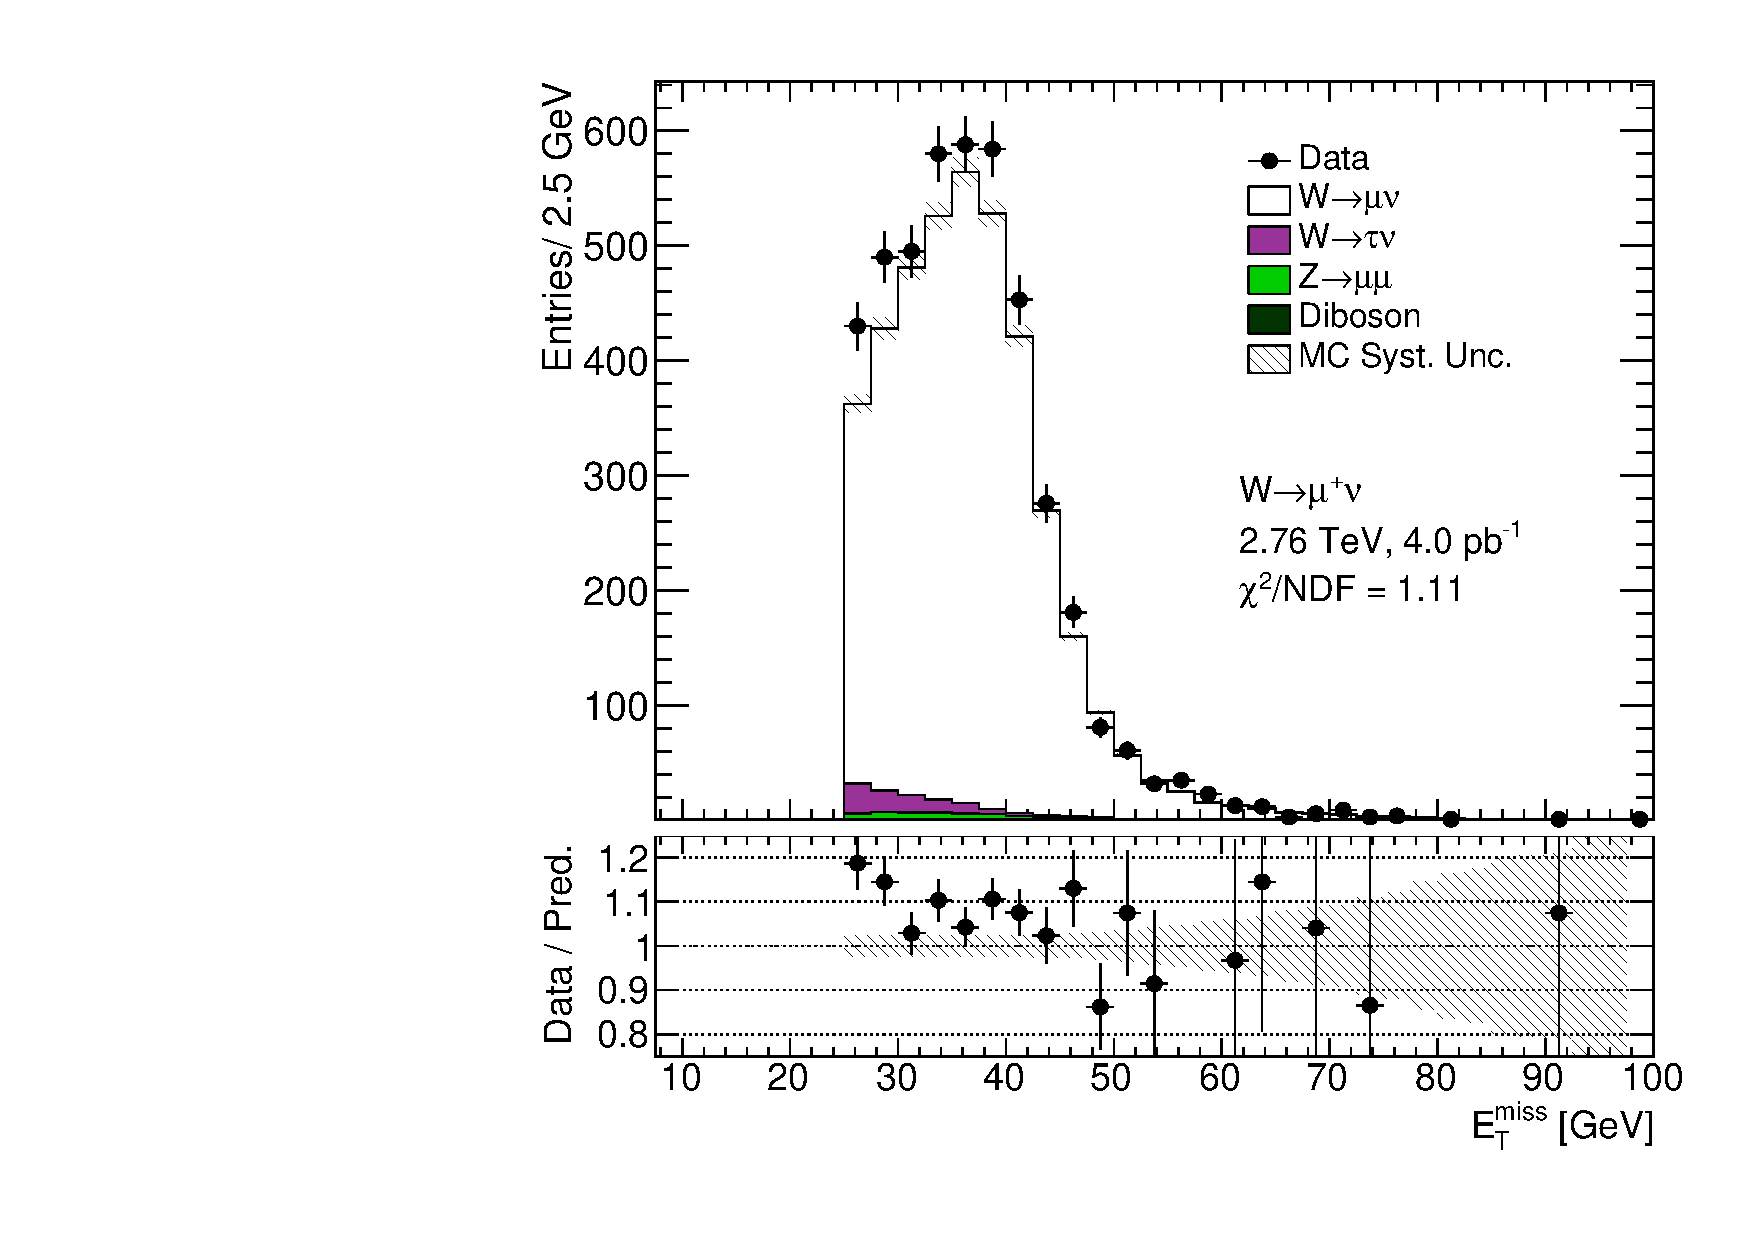
\includegraphics[width=1.\linewidth]{ControlPlots/Wanalysis/Wmu_Plus_etMiss.pdf} \\ b)}
\end{minipage}

\caption{Missing transverse energy distribution from the a) $W^{+} \to e^{+} \nu$ selection and  b) the $W^{+} \to \mu^{+} \nu$ selection.}
\end{figure}

\begin{figure}[h]
\begin{minipage}[h]{0.49\linewidth}
\center{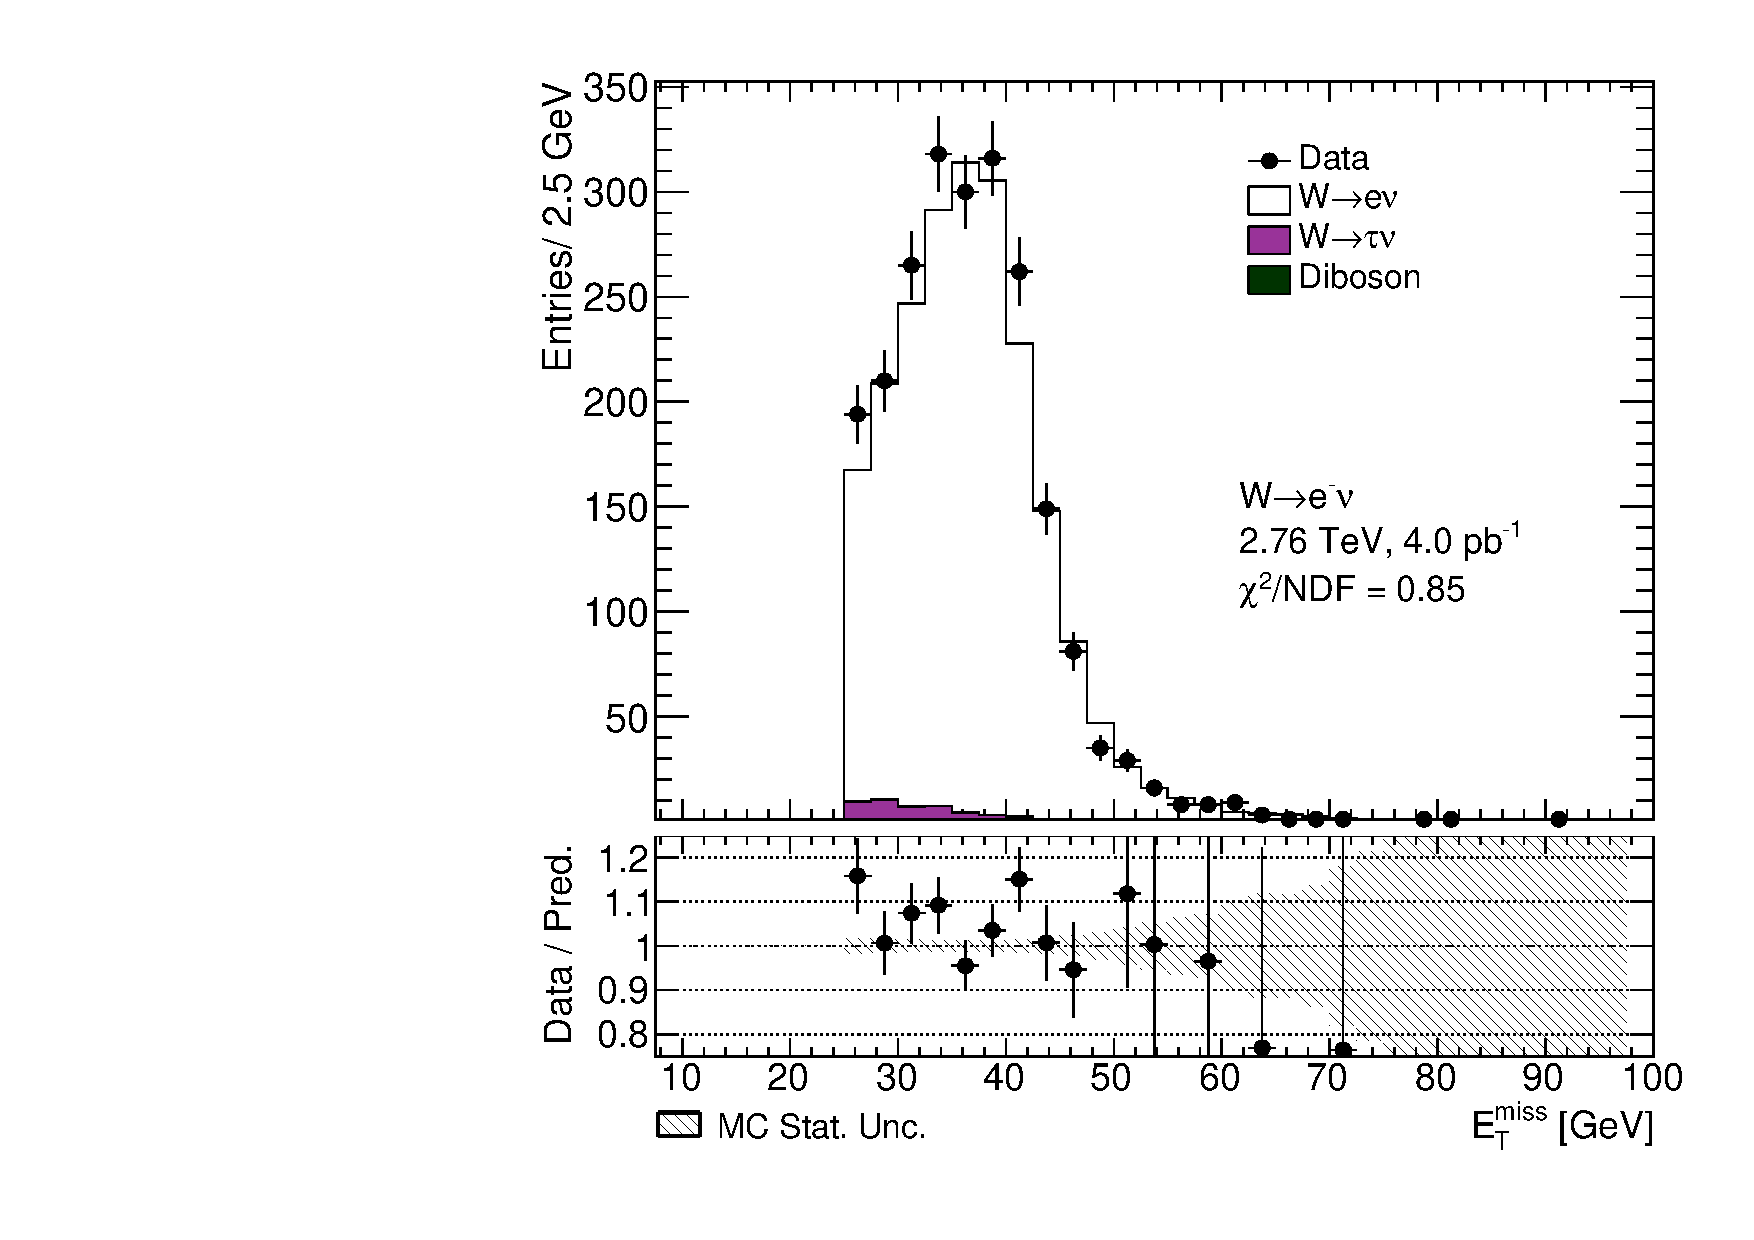
\includegraphics[width=1.\linewidth]{ControlPlots/Wanalysis/W_Minus_etMiss.pdf} \\ a)}
\end{minipage}
\hfill
\begin{minipage}[h]{0.49\linewidth}
\center{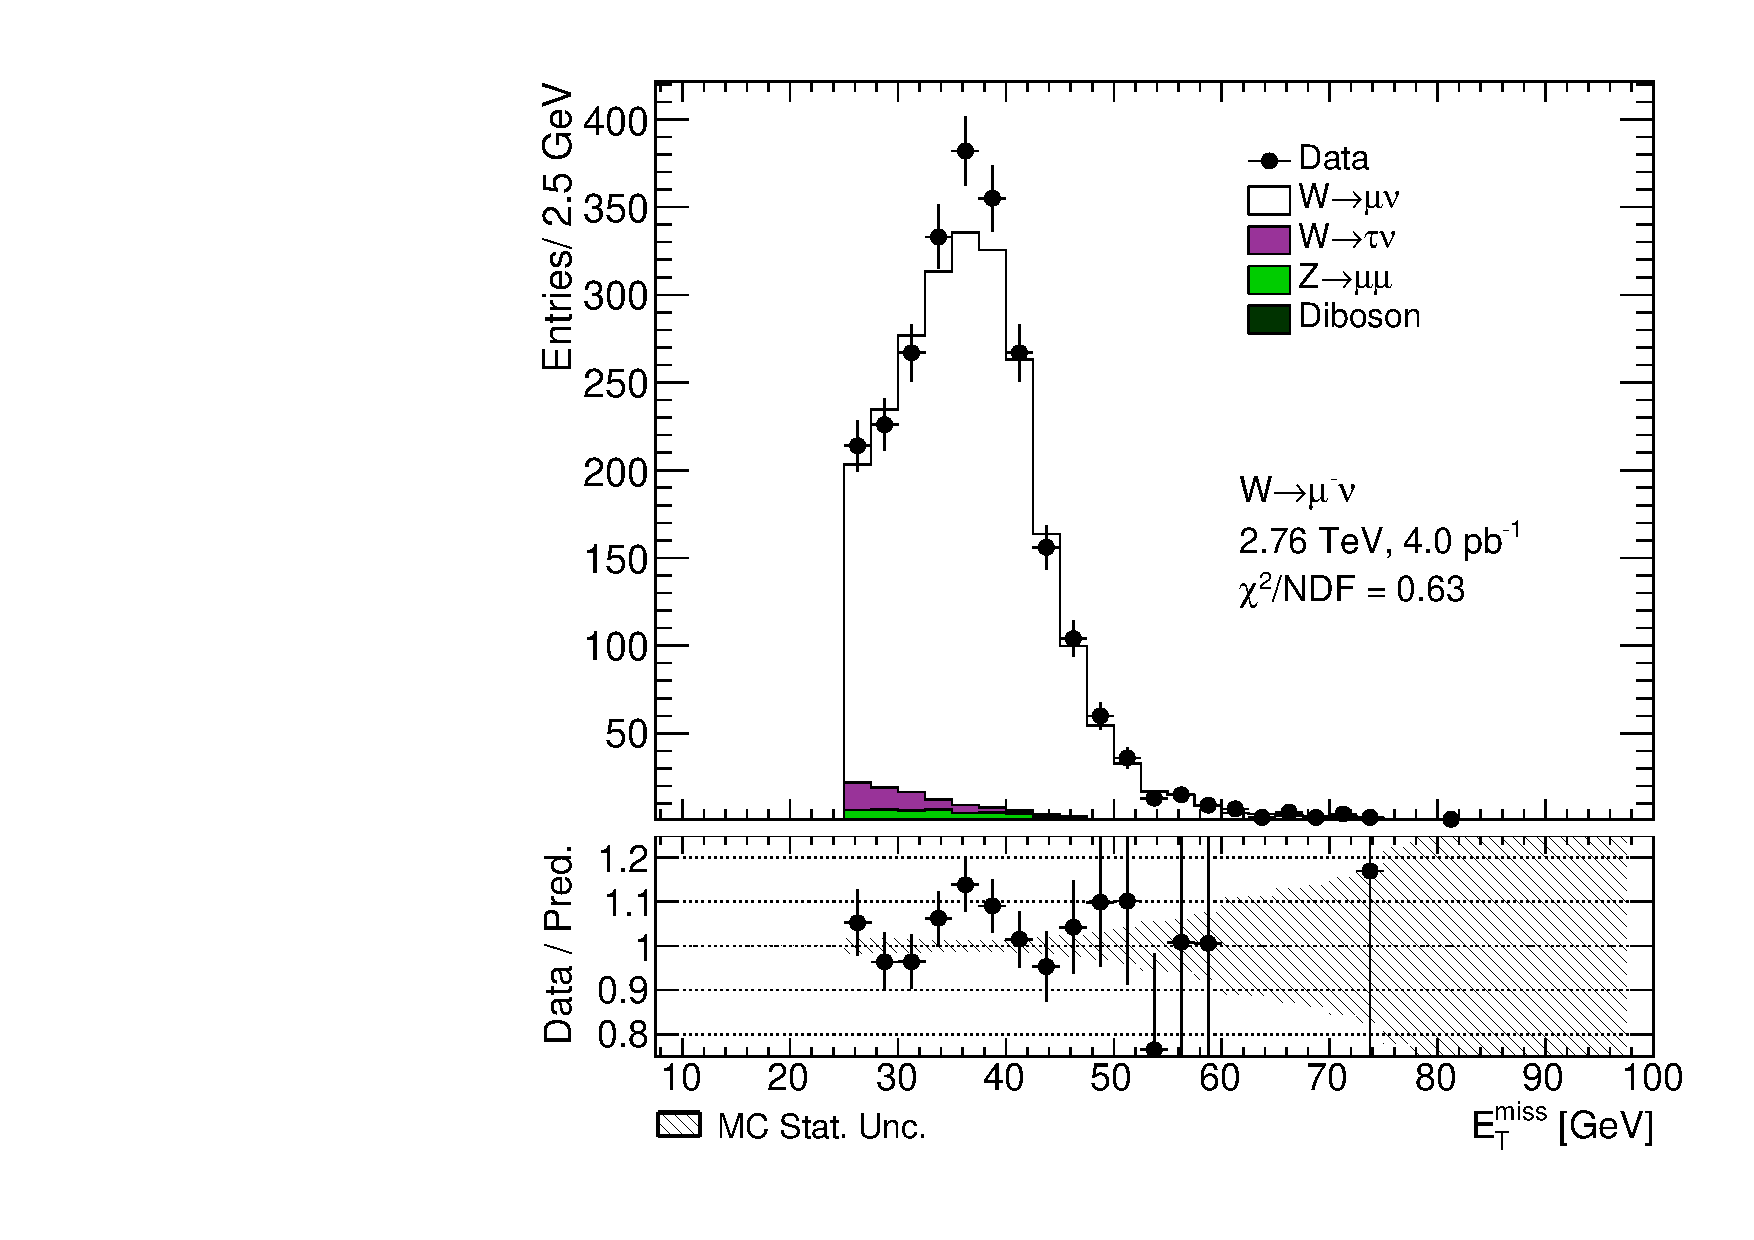
\includegraphics[width=1.\linewidth]{ControlPlots/Wanalysis/Wmu_Minus_etMiss.pdf} \\ b)}
\end{minipage}

\caption{Missing transverse energy distribution from the a) $W^{-} \to e^{-} \nu$ selection and  b) the $W^{-} \to \mu^{-} \nu$ selection.}
\end{figure}

%============================================================================================================
% mtW

\begin{figure}[h]
\begin{minipage}[h]{0.49\linewidth}
\center{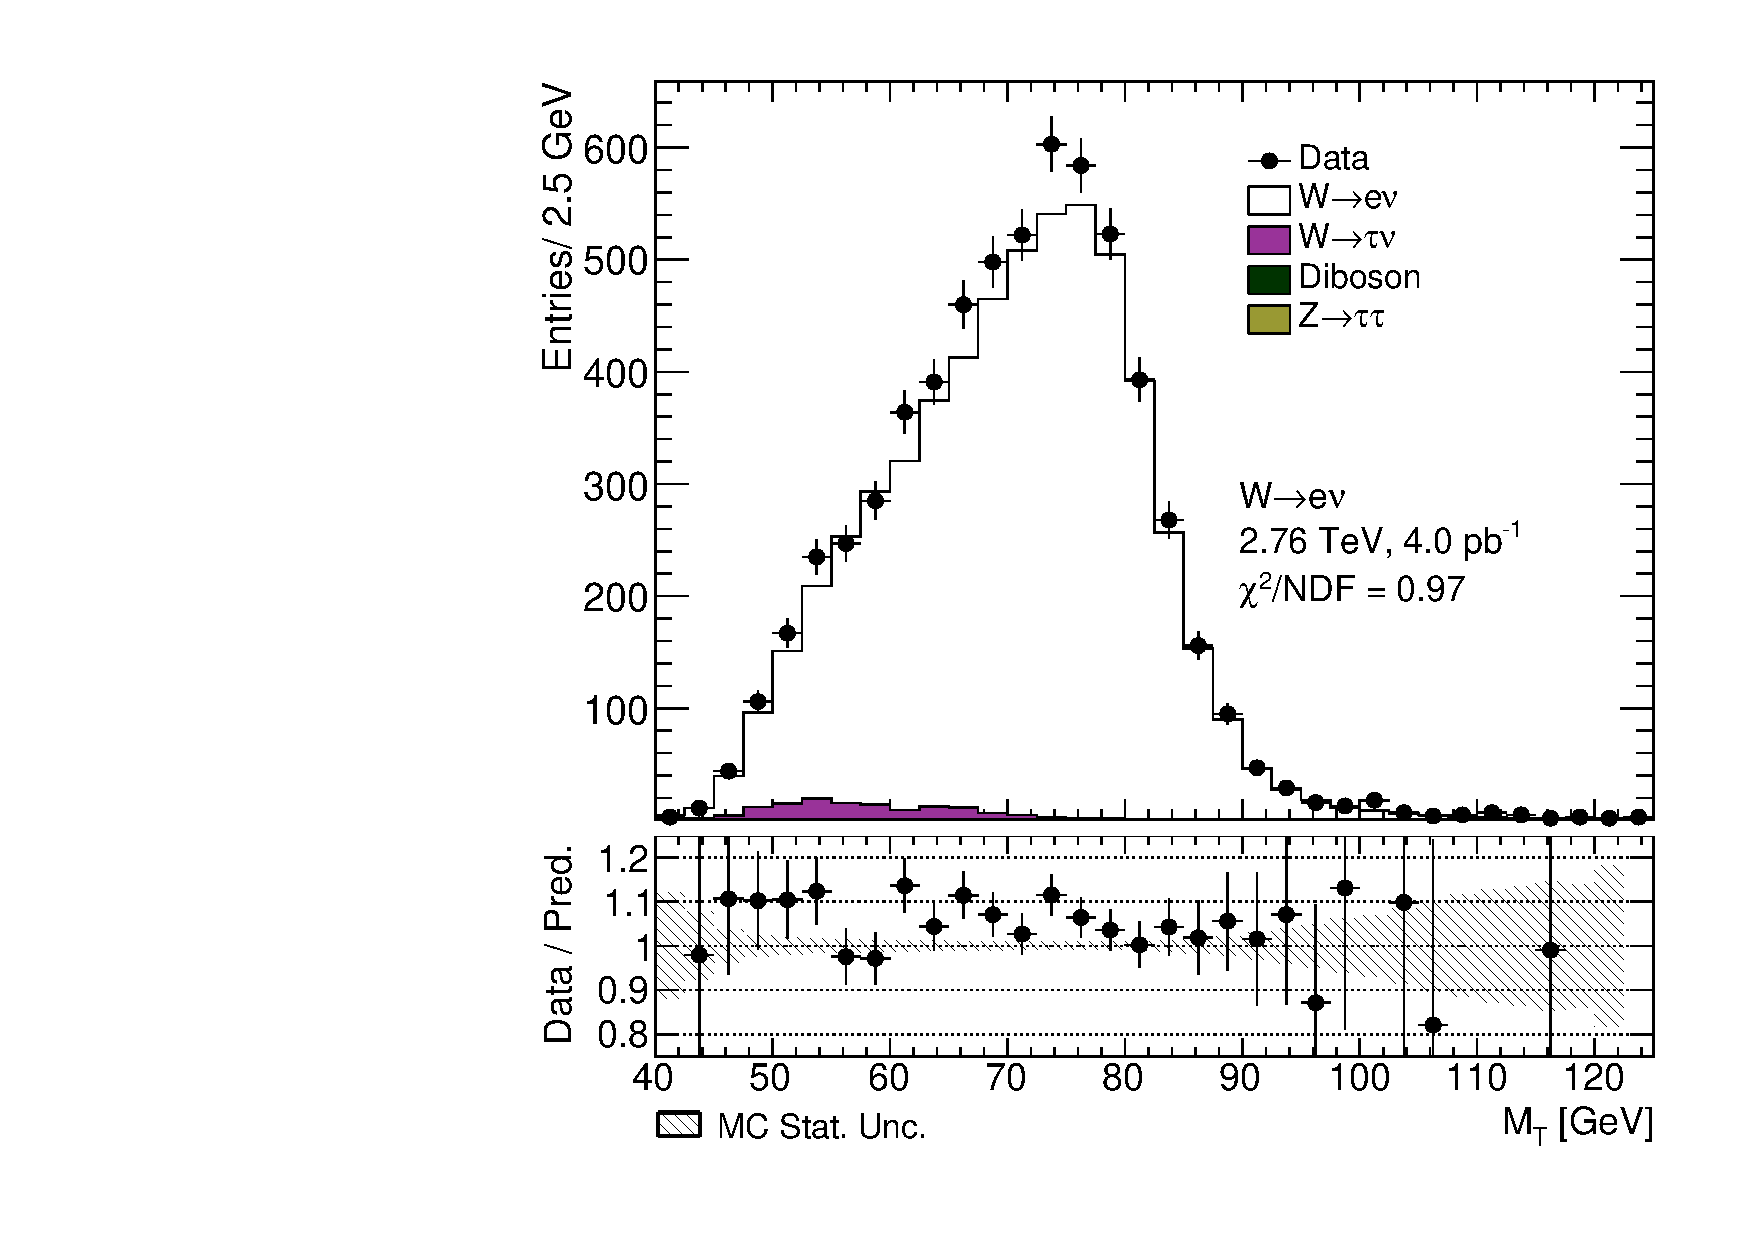
\includegraphics[width=1.\linewidth]{ControlPlots/Wanalysis/W_Boson_mtW.pdf} \\ a)}
\end{minipage}
\hfill
\begin{minipage}[h]{0.49\linewidth}
\center{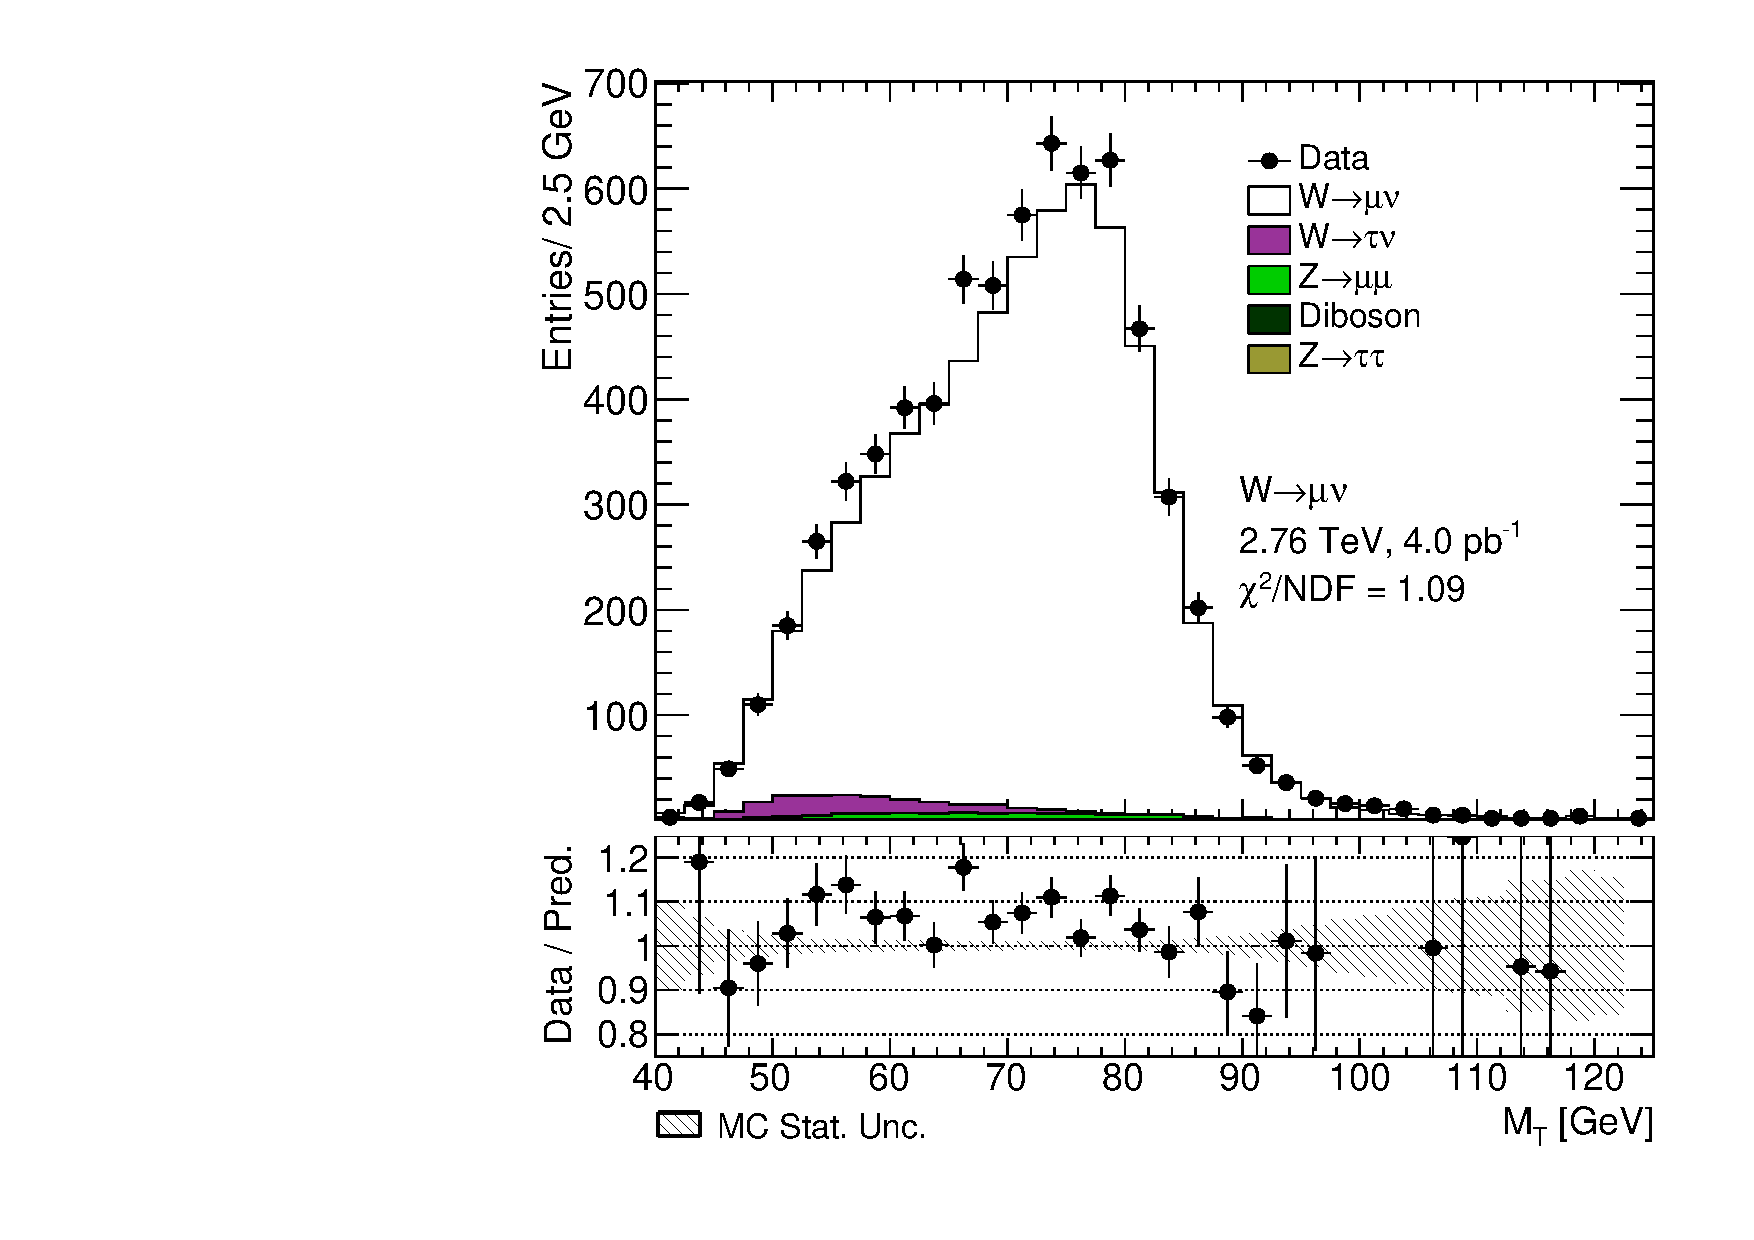
\includegraphics[width=1.\linewidth]{ControlPlots/Wanalysis/Wmu_Boson_mtW.pdf} \\ b)}
\end{minipage}

\caption{Transverse mass distribution distribution from the a) \wenu selection and  b) the \wmunu selection.}
\end{figure}

\begin{figure}[h]
\begin{minipage}[h]{0.49\linewidth}
\center{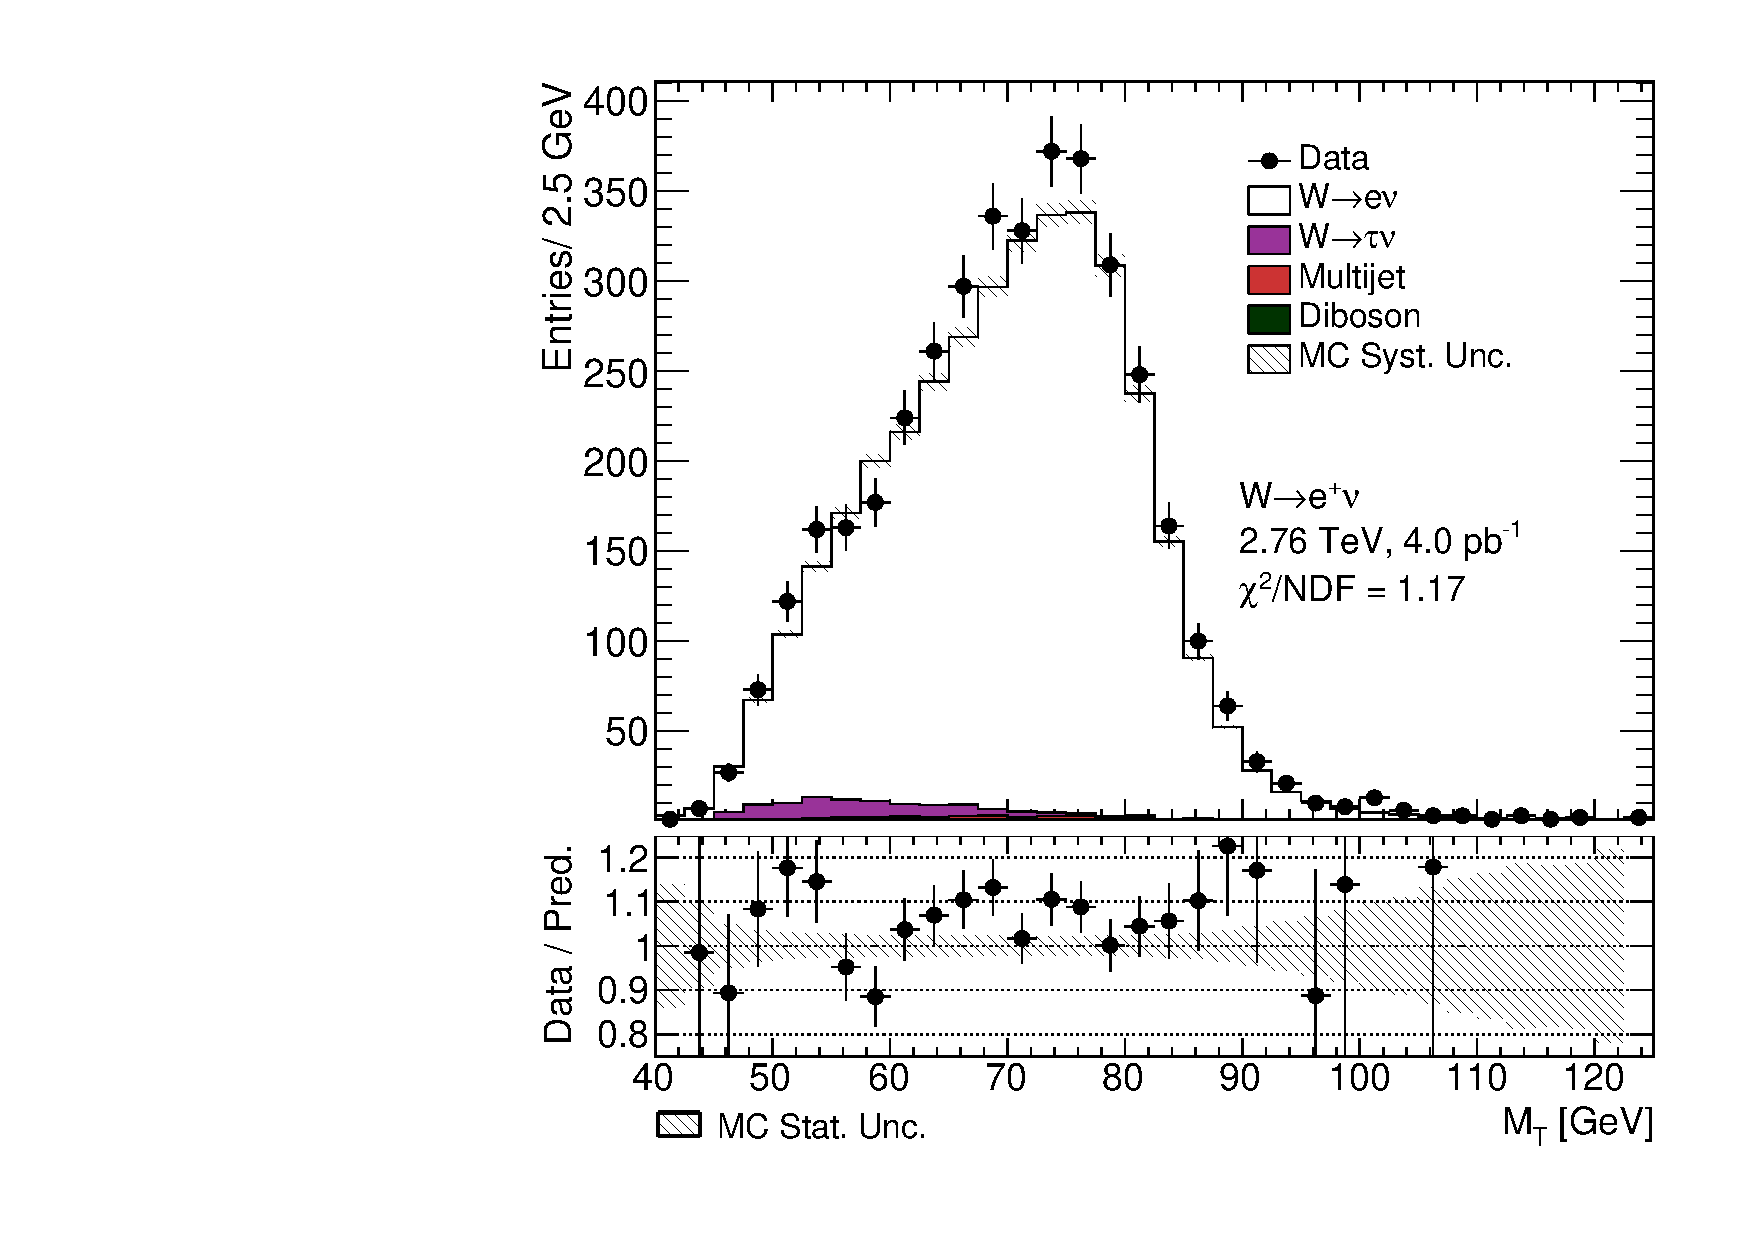
\includegraphics[width=1.\linewidth]{ControlPlots/Wanalysis/W_Plus_mtW.pdf} \\ a)}
\end{minipage}
\hfill
\begin{minipage}[h]{0.49\linewidth}
\center{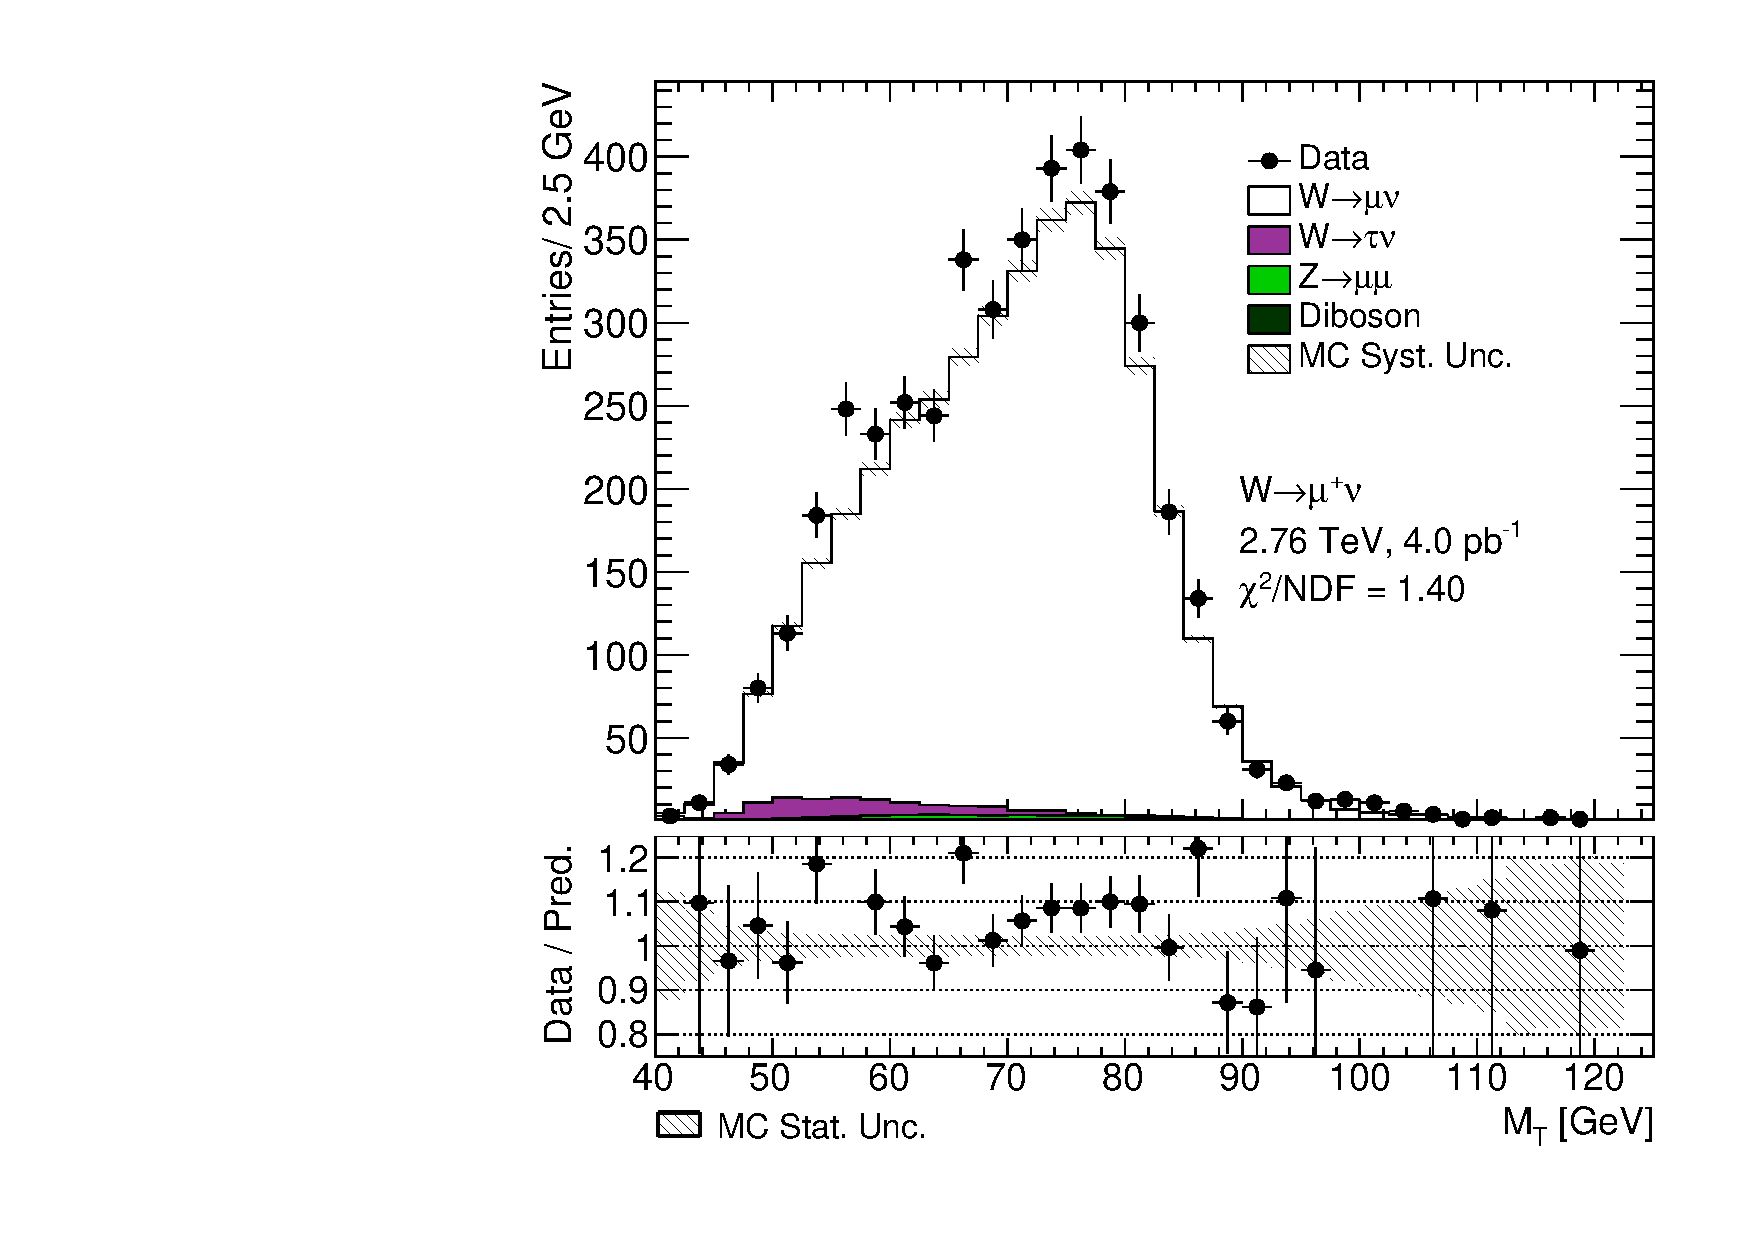
\includegraphics[width=1.\linewidth]{ControlPlots/Wanalysis/Wmu_Plus_mtW.pdf} \\ b)}
\end{minipage}

\caption{Transverse mass distribution distribution from the a) $W^{+} \to e^{+} \nu$ selection and  b) the $W^{+} \to \mu^{+} \nu$ selection.}
\end{figure}

\begin{figure}[h]
\begin{minipage}[h]{0.49\linewidth}
\center{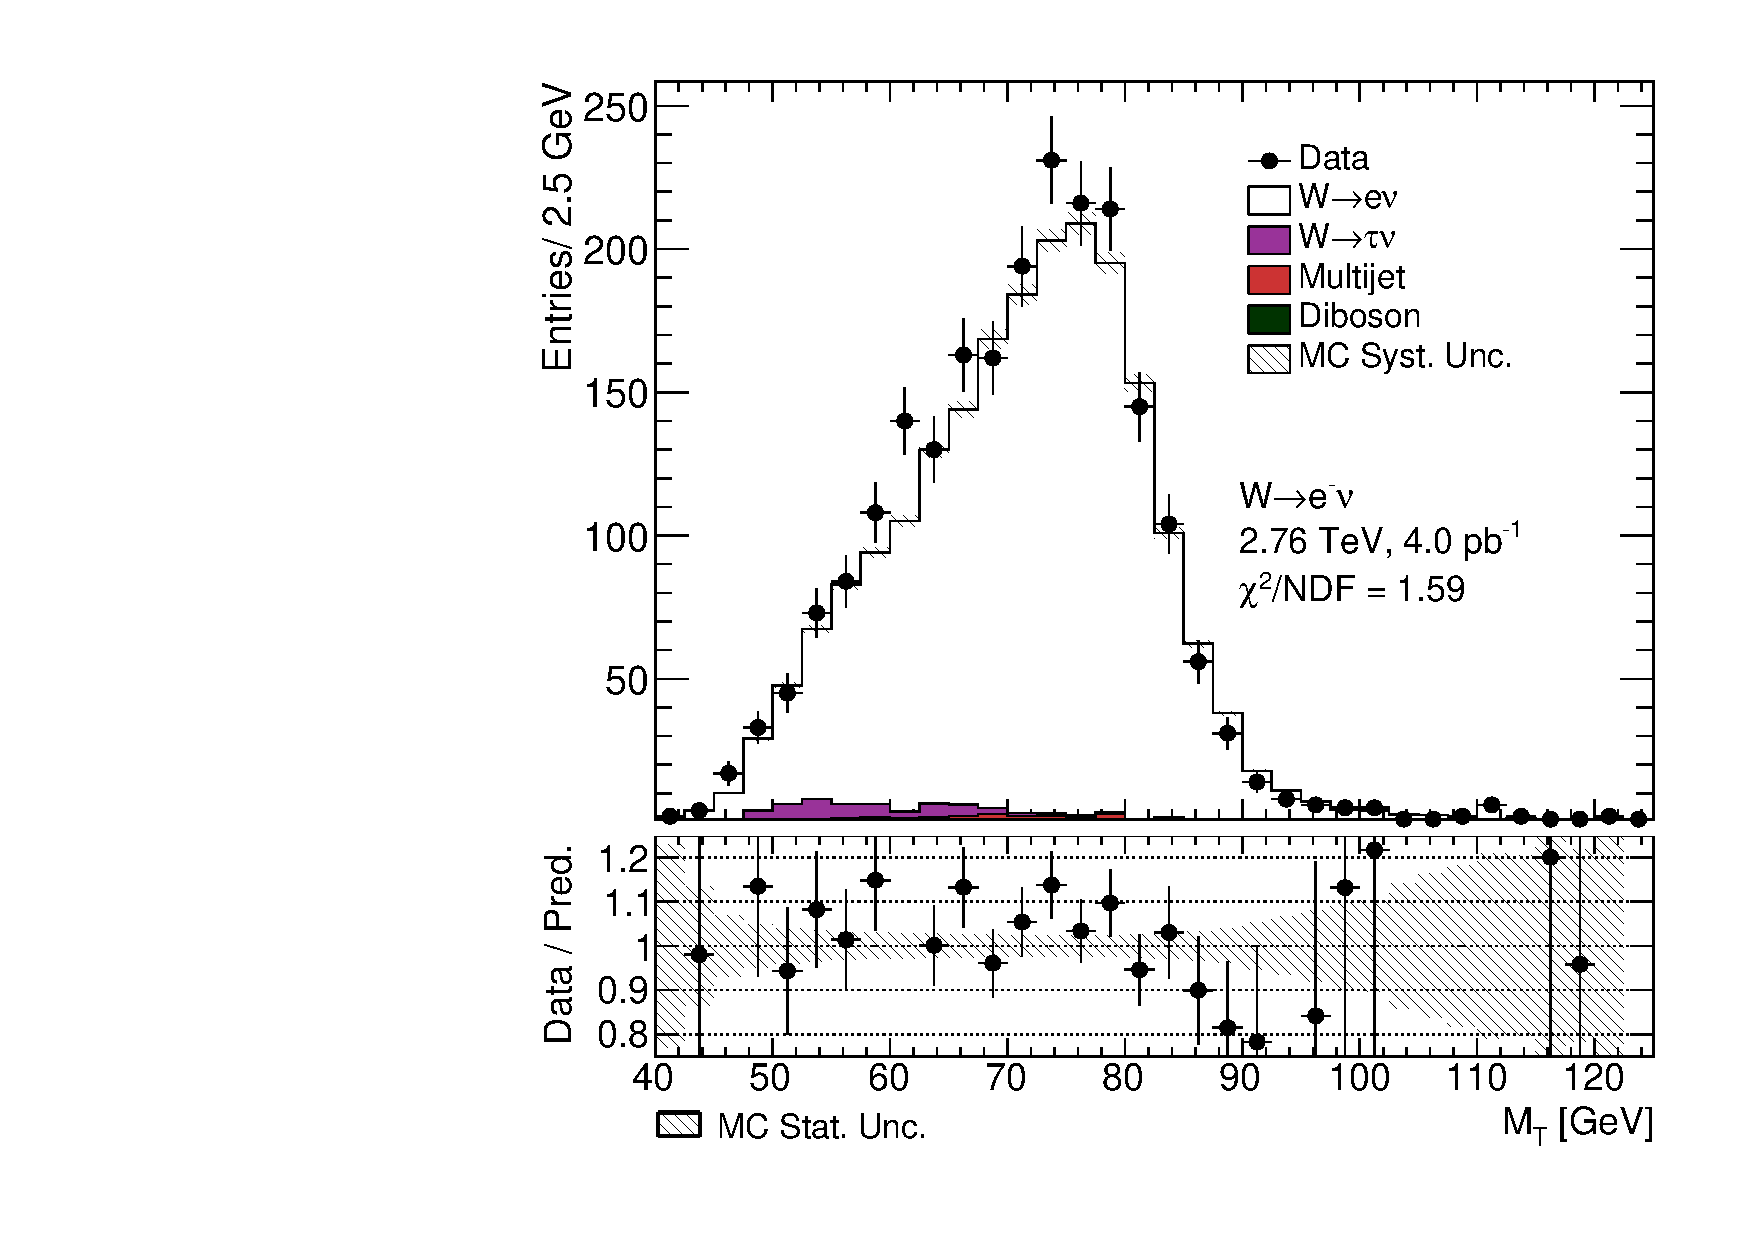
\includegraphics[width=1.\linewidth]{ControlPlots/Wanalysis/W_Minus_mtW.pdf} \\ a)}
\end{minipage}
\hfill
\begin{minipage}[h]{0.49\linewidth}
\center{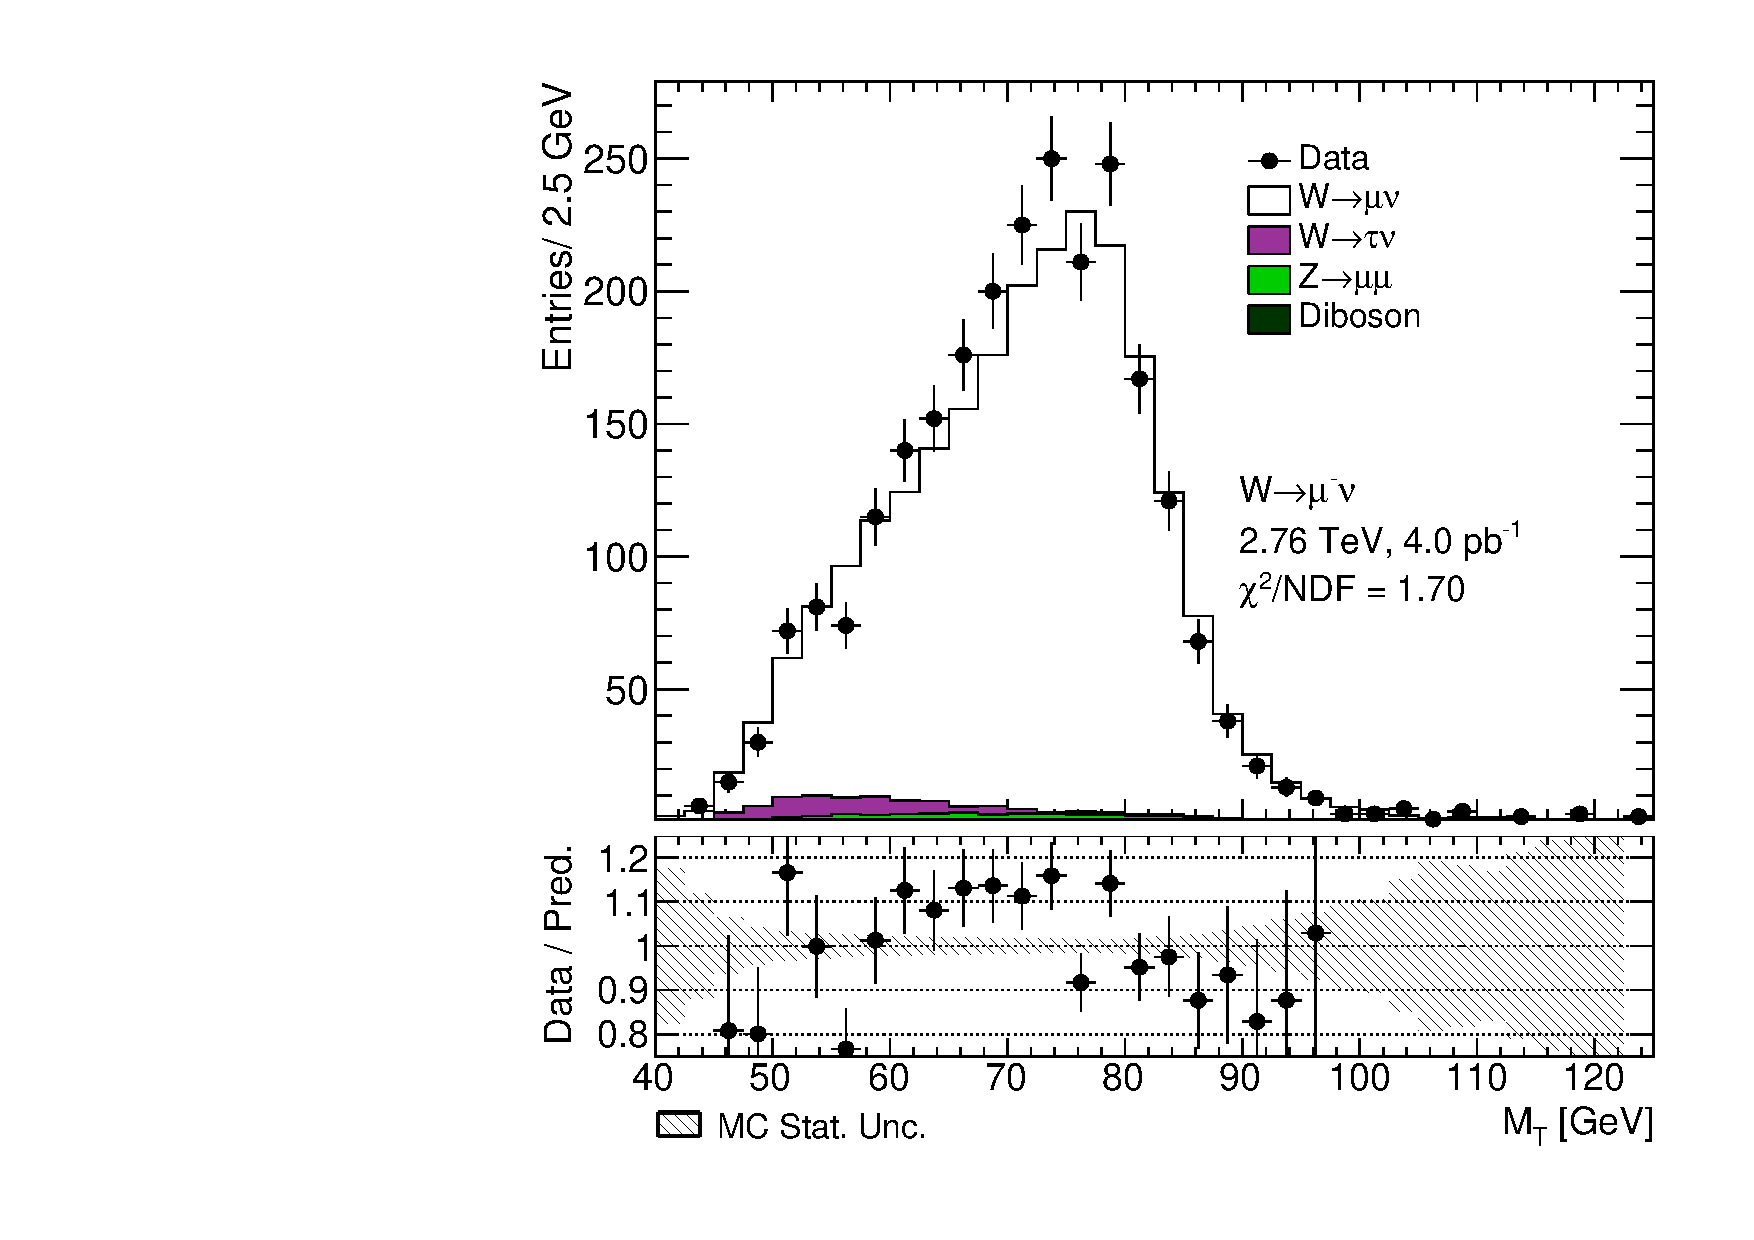
\includegraphics[width=1.\linewidth]{ControlPlots/Wanalysis/Wmu_Minus_mtW.pdf} \\ b)}
\end{minipage}
\caption{Transverse mass distribution distribution from the a) $W^{-} \to e^{-} \nu$ selection and  b) the $W^{-} \to \mu^{-} \nu$ selection.}
\label{ris:WlnumtWM}
\end{figure}

%============================================================================================================
% Zll  LepEta

\begin{figure}[h]
\begin{minipage}[h]{0.49\linewidth}
\center{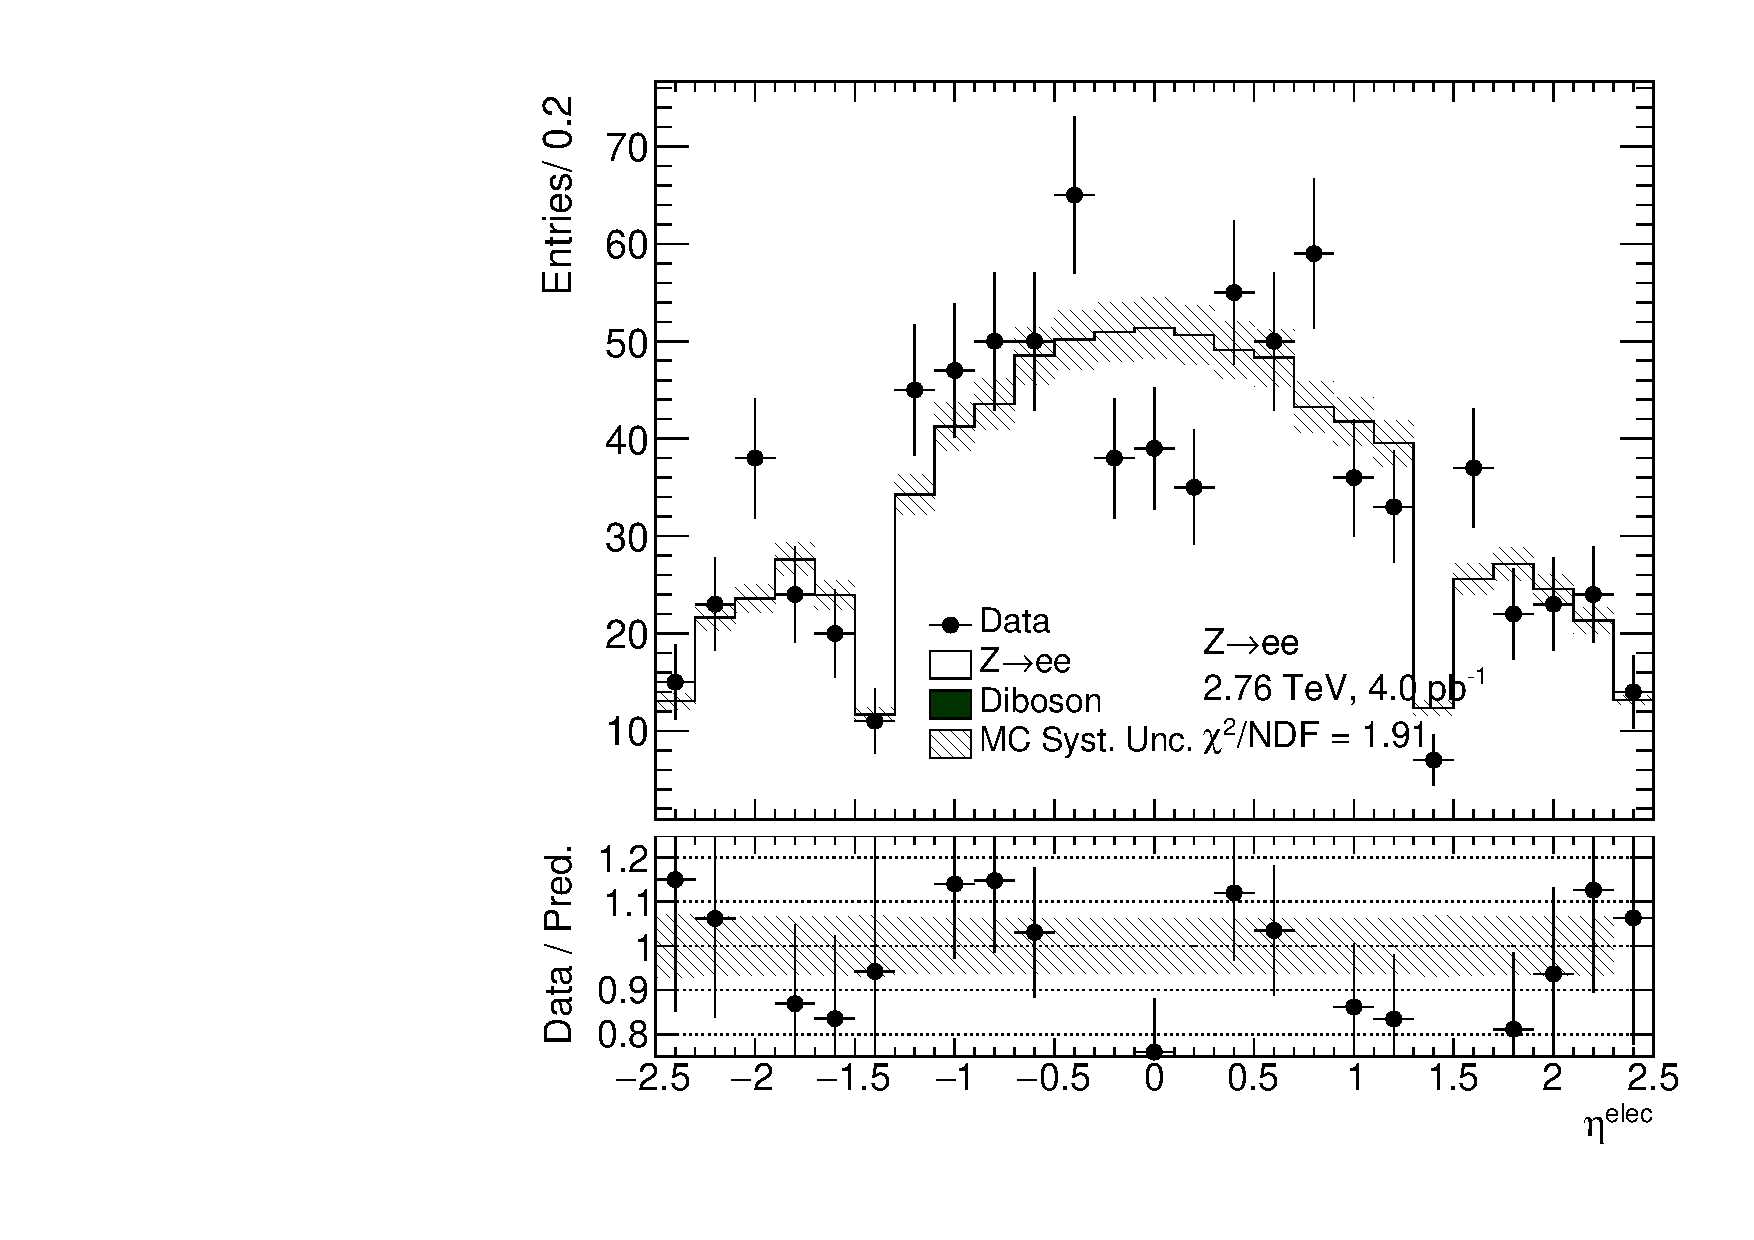
\includegraphics[width=1.\linewidth]{ControlPlots/Zanalysis/ZCC_Electron_ElecEta.pdf} \\ a)}
\end{minipage}
\hfill
\begin{minipage}[h]{0.49\linewidth}
\center{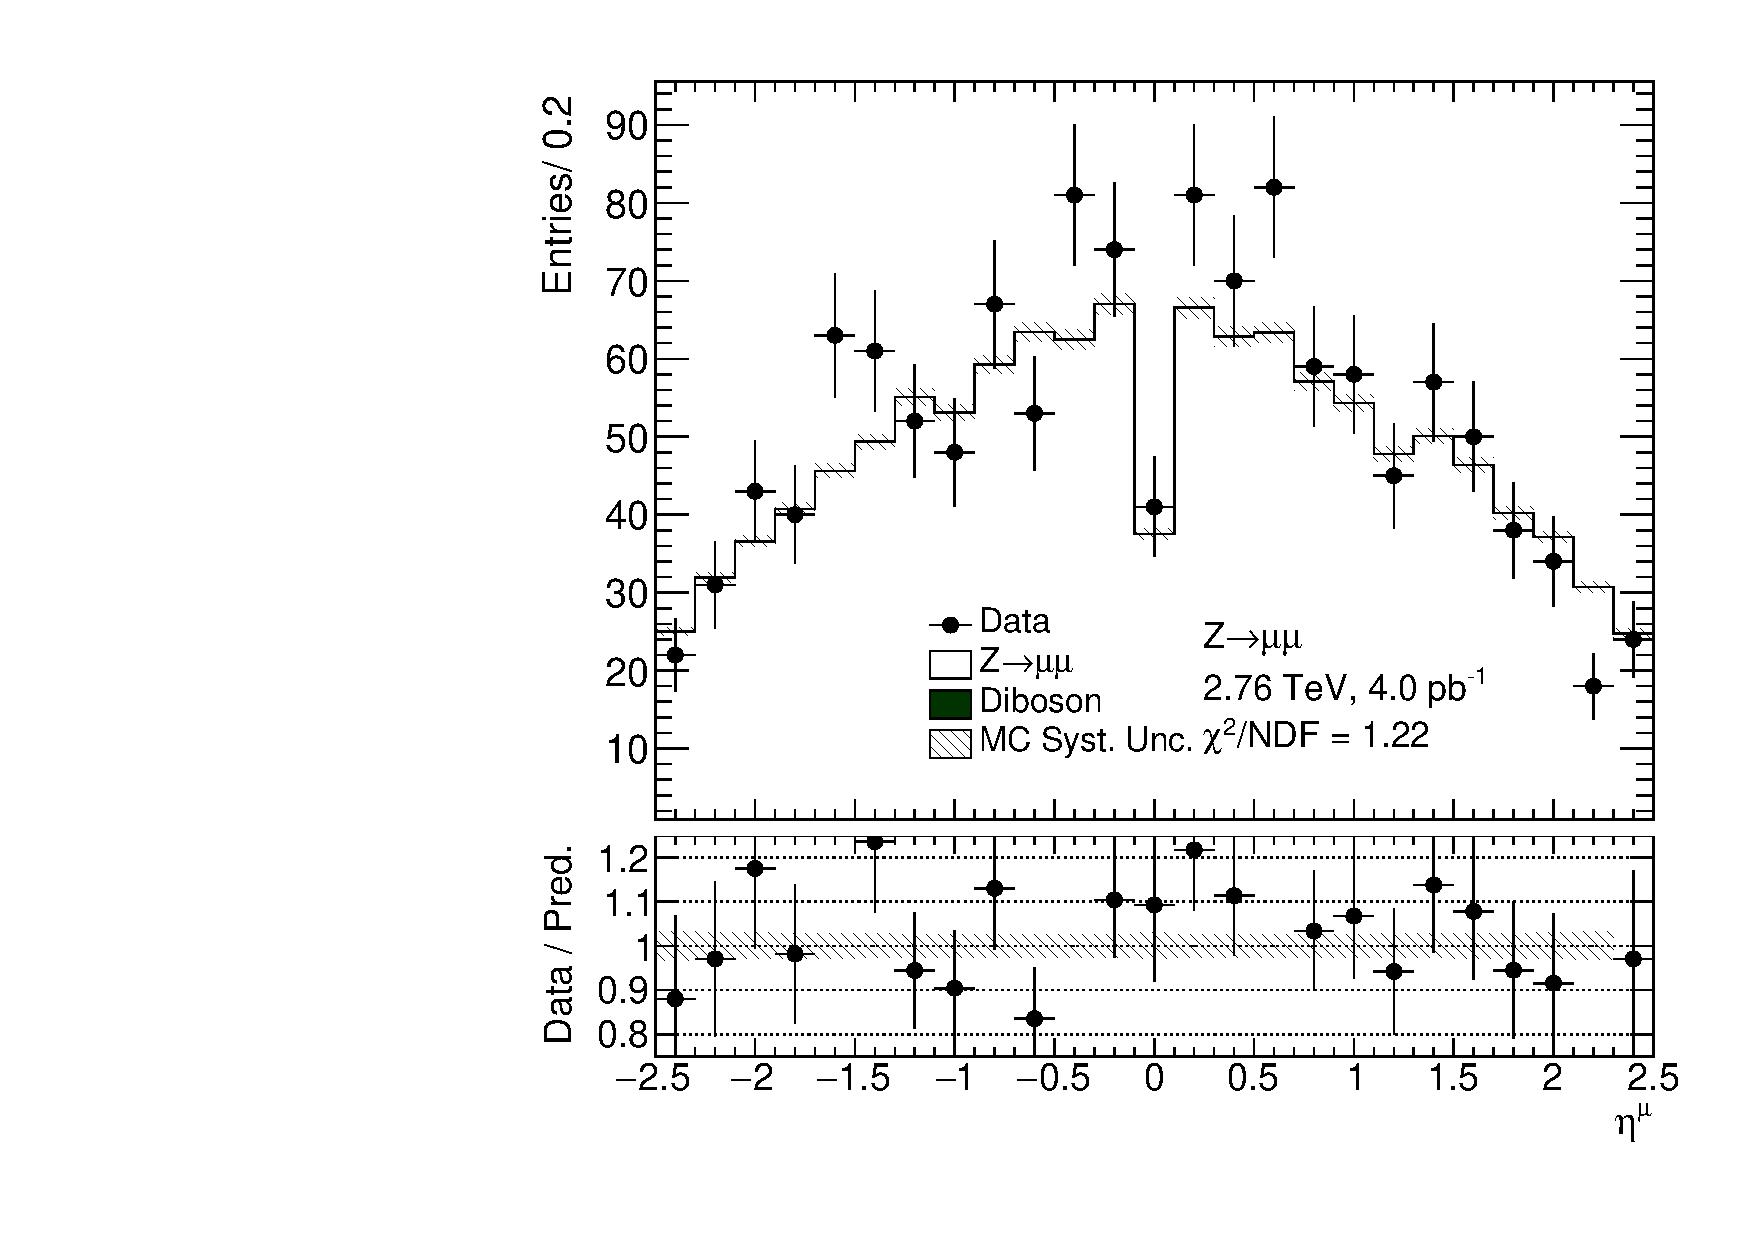
\includegraphics[width=1.\linewidth]{ControlPlots/Zanalysis/Zmumu_Muon_Eta.pdf} \\ b)}
\end{minipage}
\caption{ Lepton pseudorapidity distributions from the a) $Z\to e^{+}e^{-}$ b) $Z\to \mu^{+}\mu^{-}$.}
\label{ris:Zll}
\end{figure}

\begin{figure}[h]
\begin{minipage}[h]{0.49\linewidth}
\center{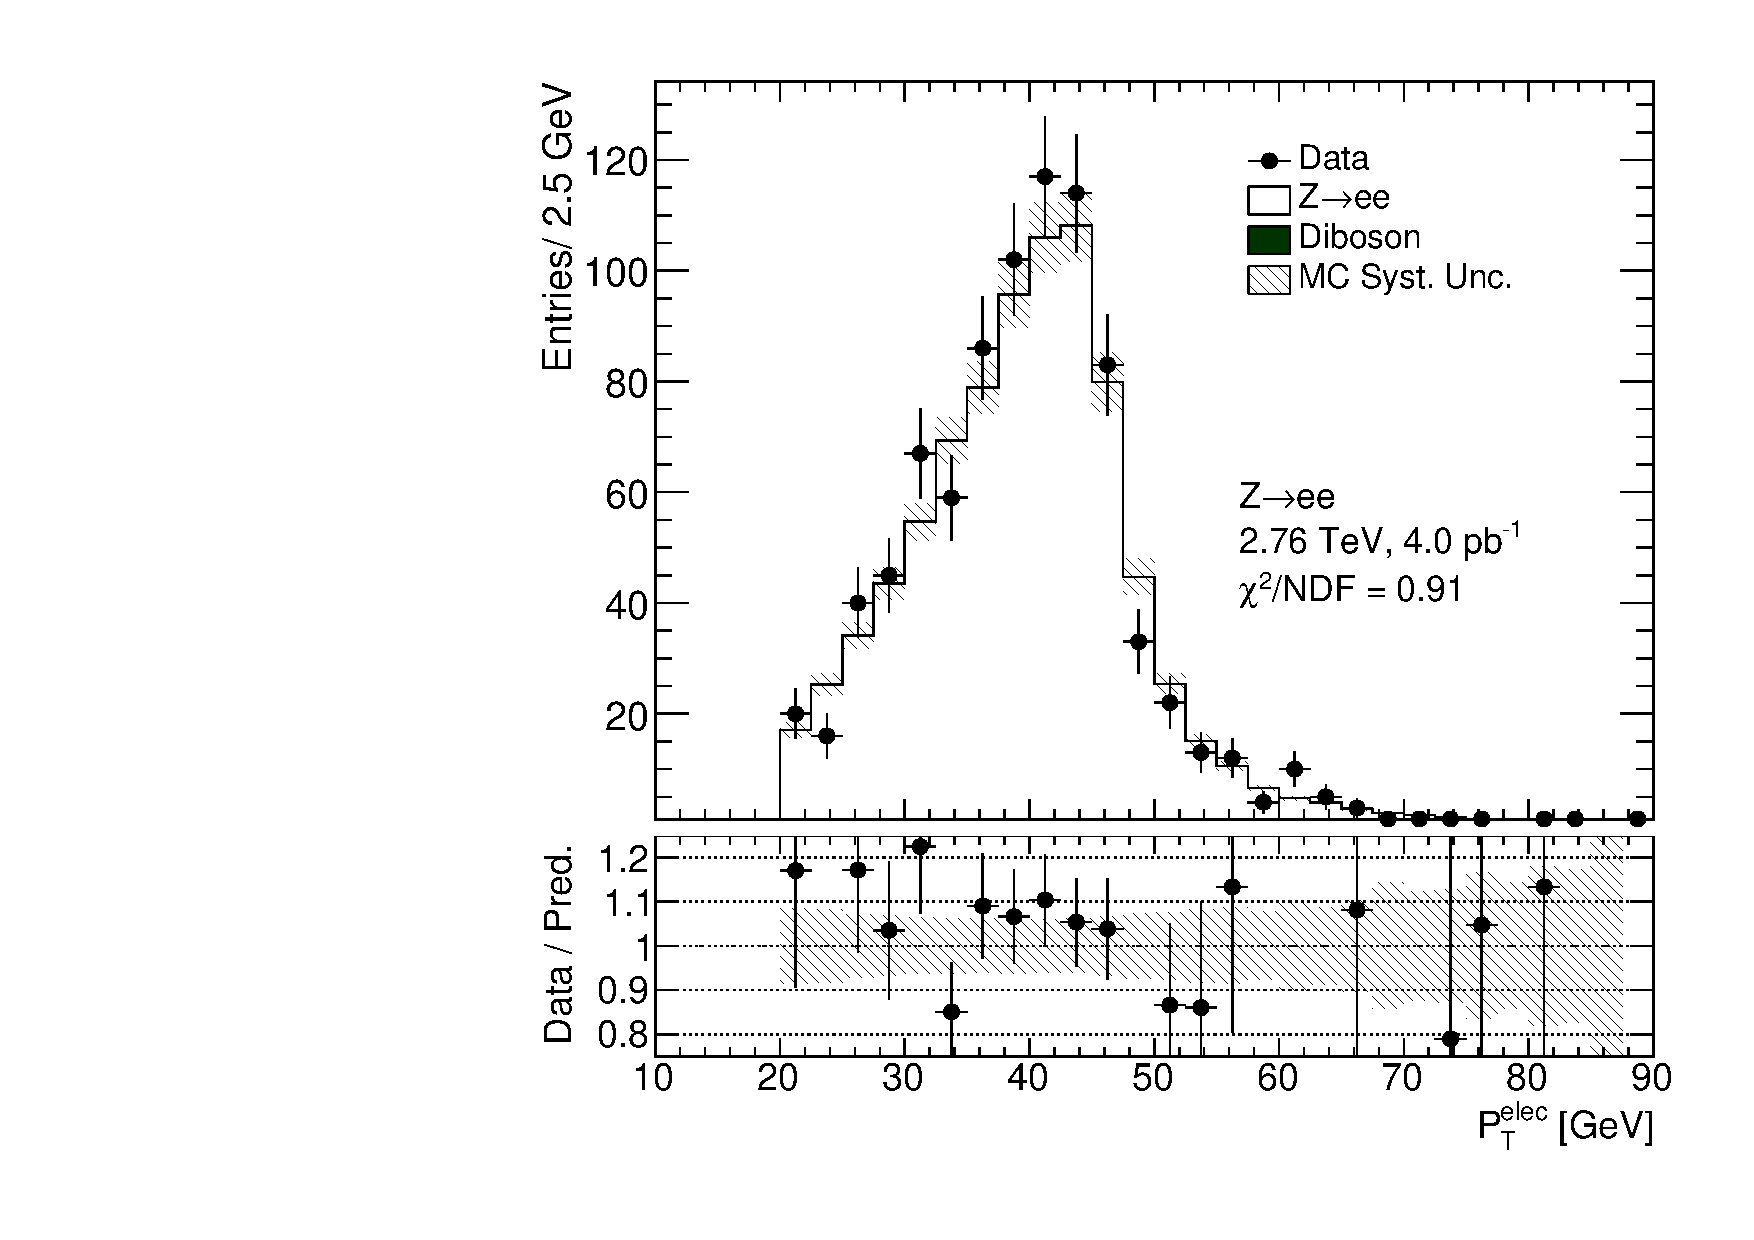
\includegraphics[width=1.\linewidth]{ControlPlots/Zanalysis/ZCC_Electron_ElecPt.pdf} \\ a)}
\end{minipage}
\hfill
\begin{minipage}[h]{0.49\linewidth}
\center{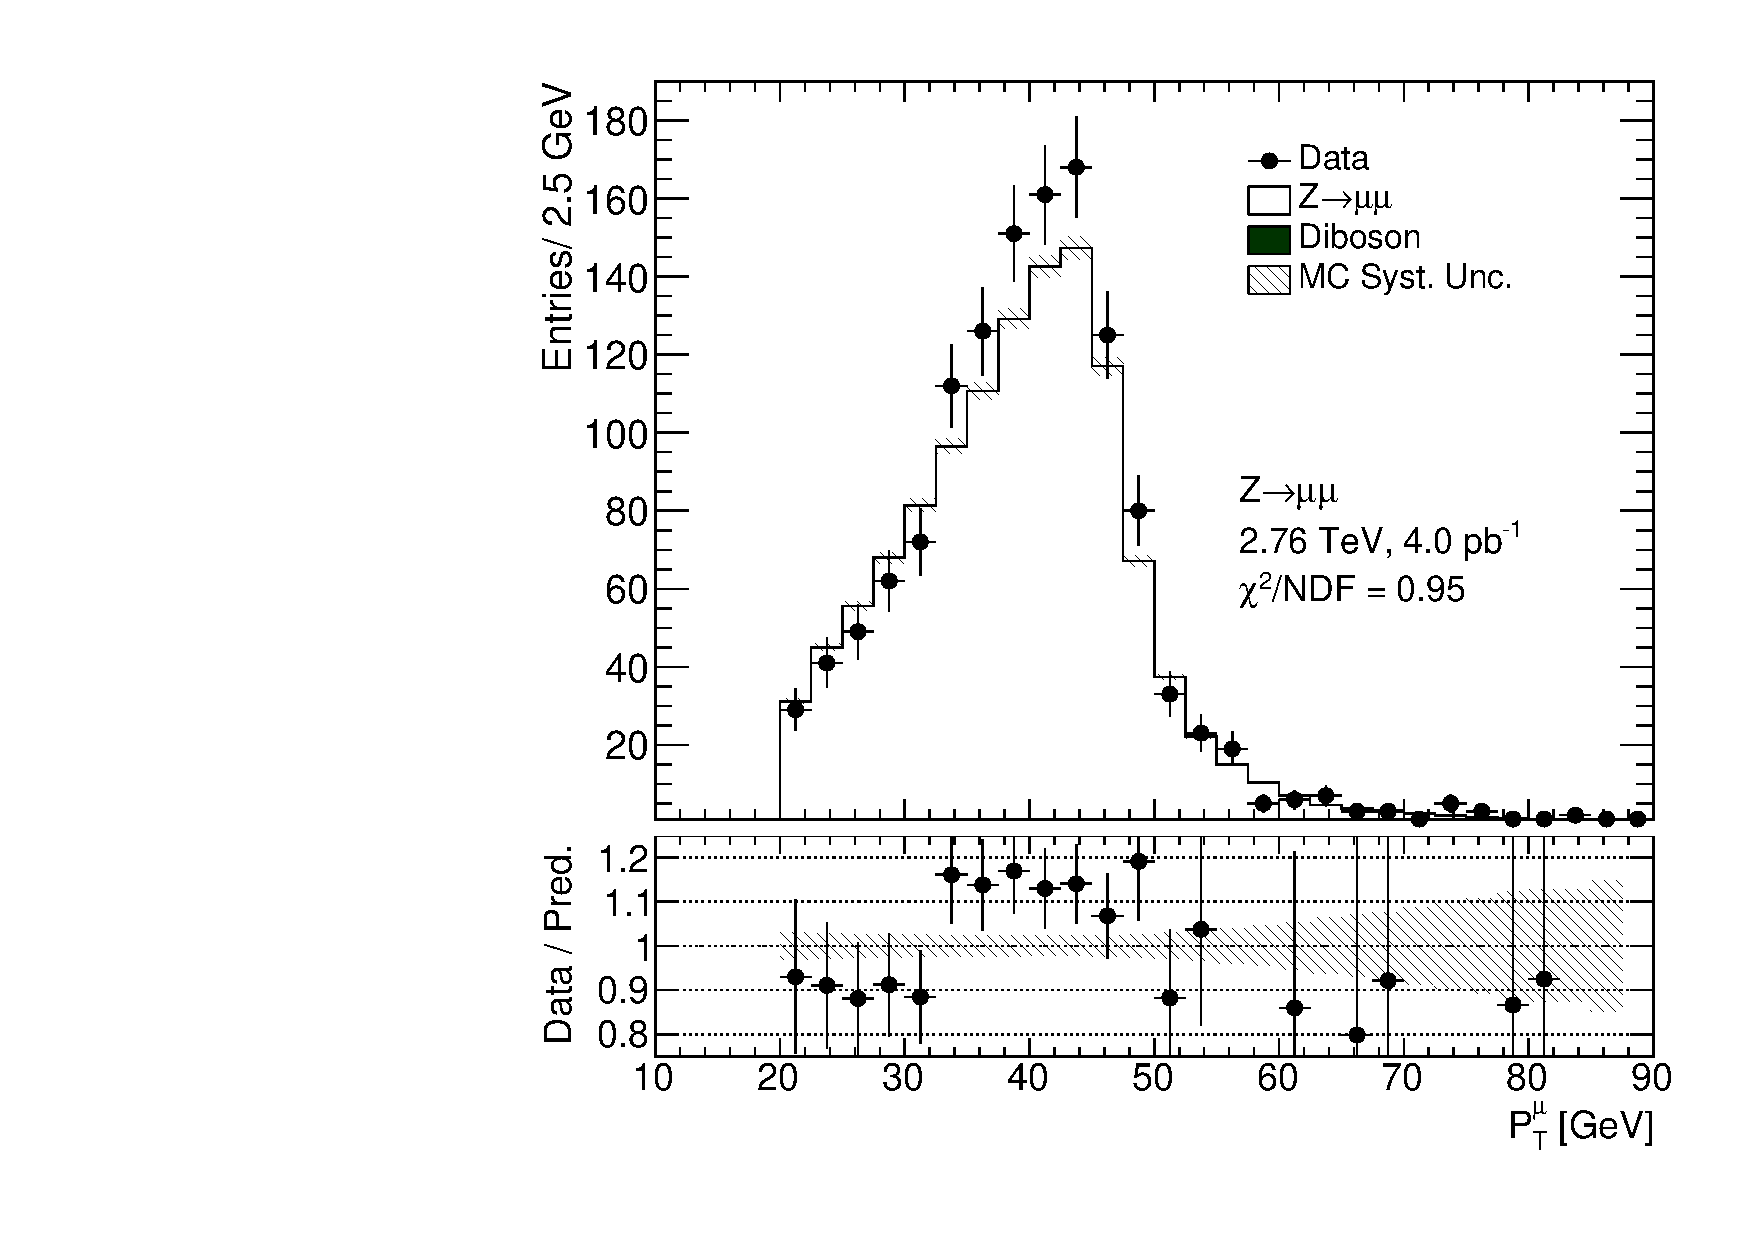
\includegraphics[width=1.\linewidth]{ControlPlots/Zanalysis/Zmumu_Muon_Pt.pdf} \\ a)}
\end{minipage}
\caption{Lepton transverse momentum distributions from the a) $Z\to e^{+}e^{-}$ b) $Z\to \mu^{+}\mu^{-}$.}

\end{figure}

\begin{figure}[h]
\begin{minipage}[h]{0.49\linewidth}
\center{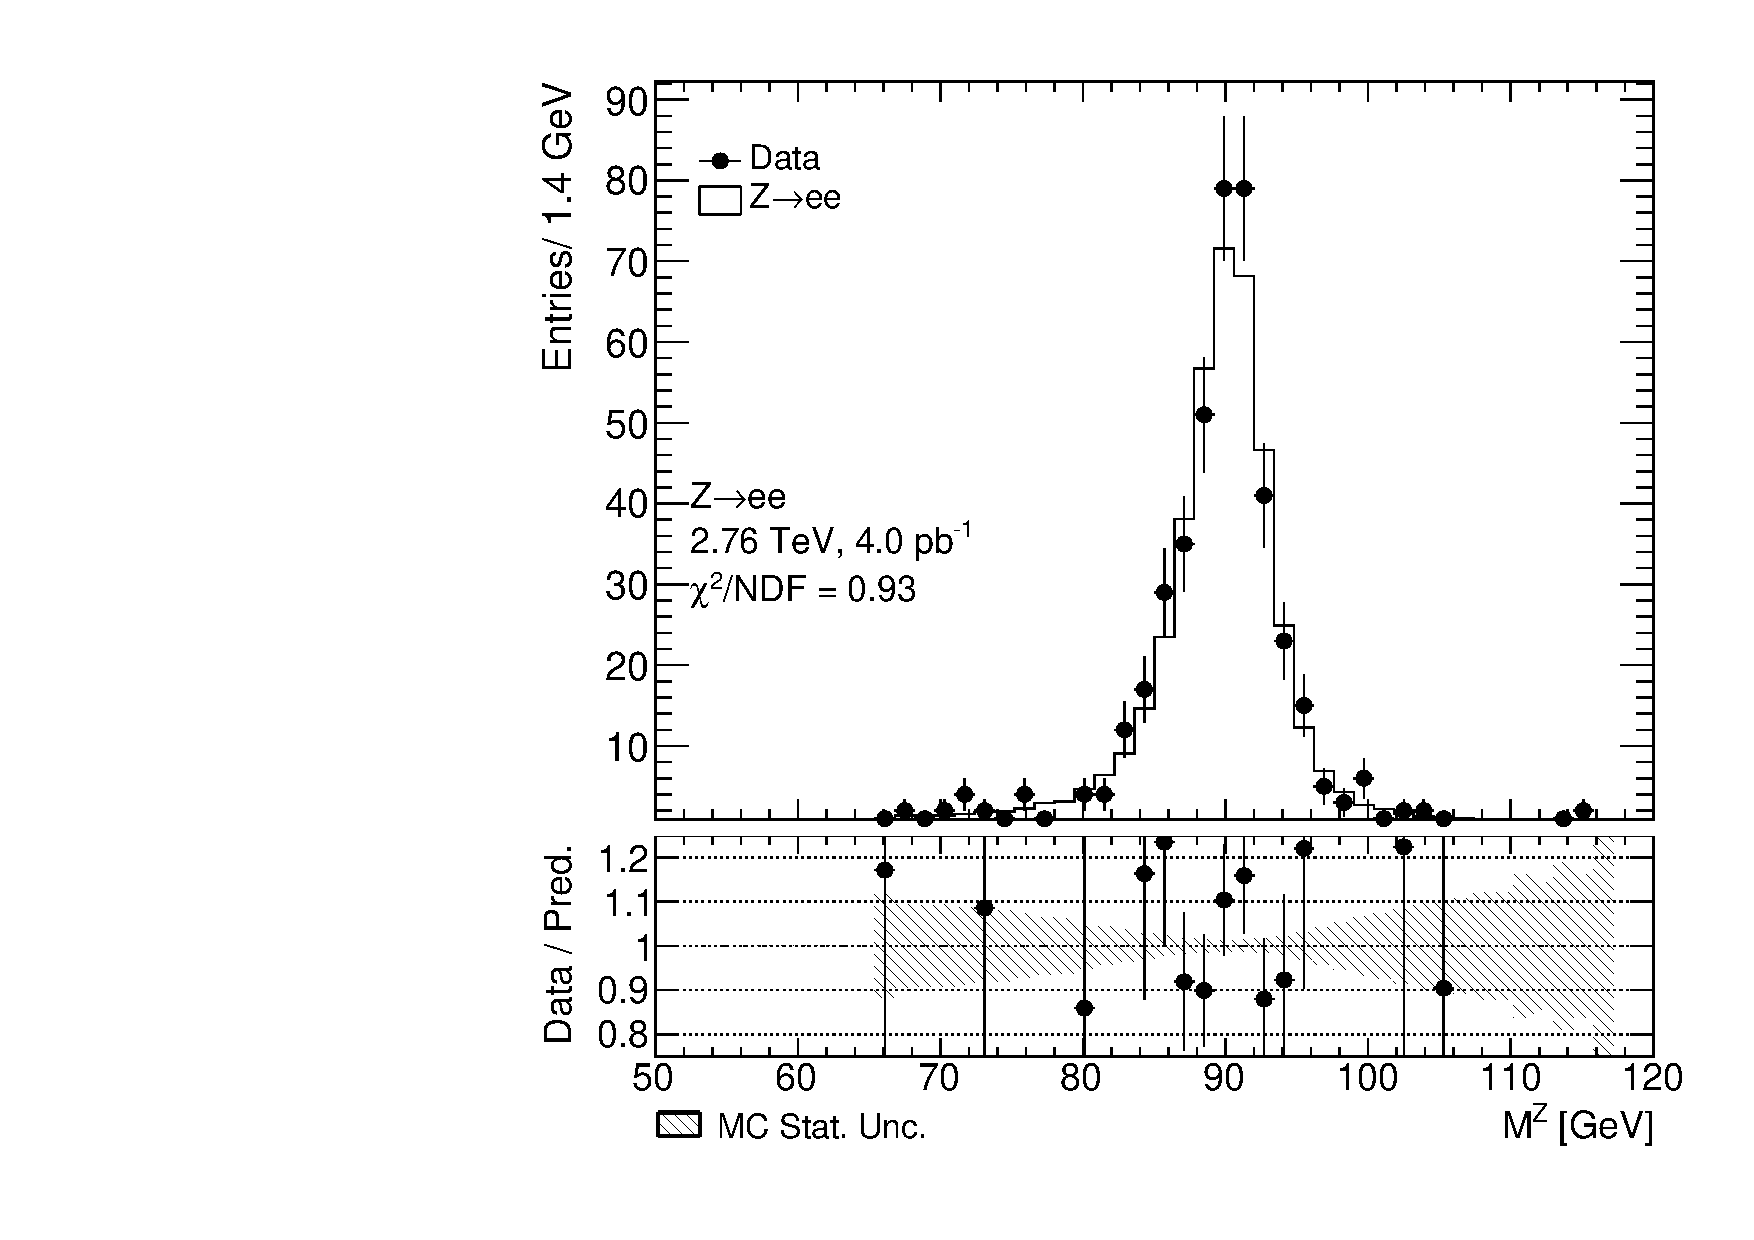
\includegraphics[width=1.\linewidth]{ControlPlots/Zanalysis/ZCC_Boson_BosMass.pdf} \\ a)}
\end{minipage}
\hfill
\begin{minipage}[h]{0.49\linewidth}
\center{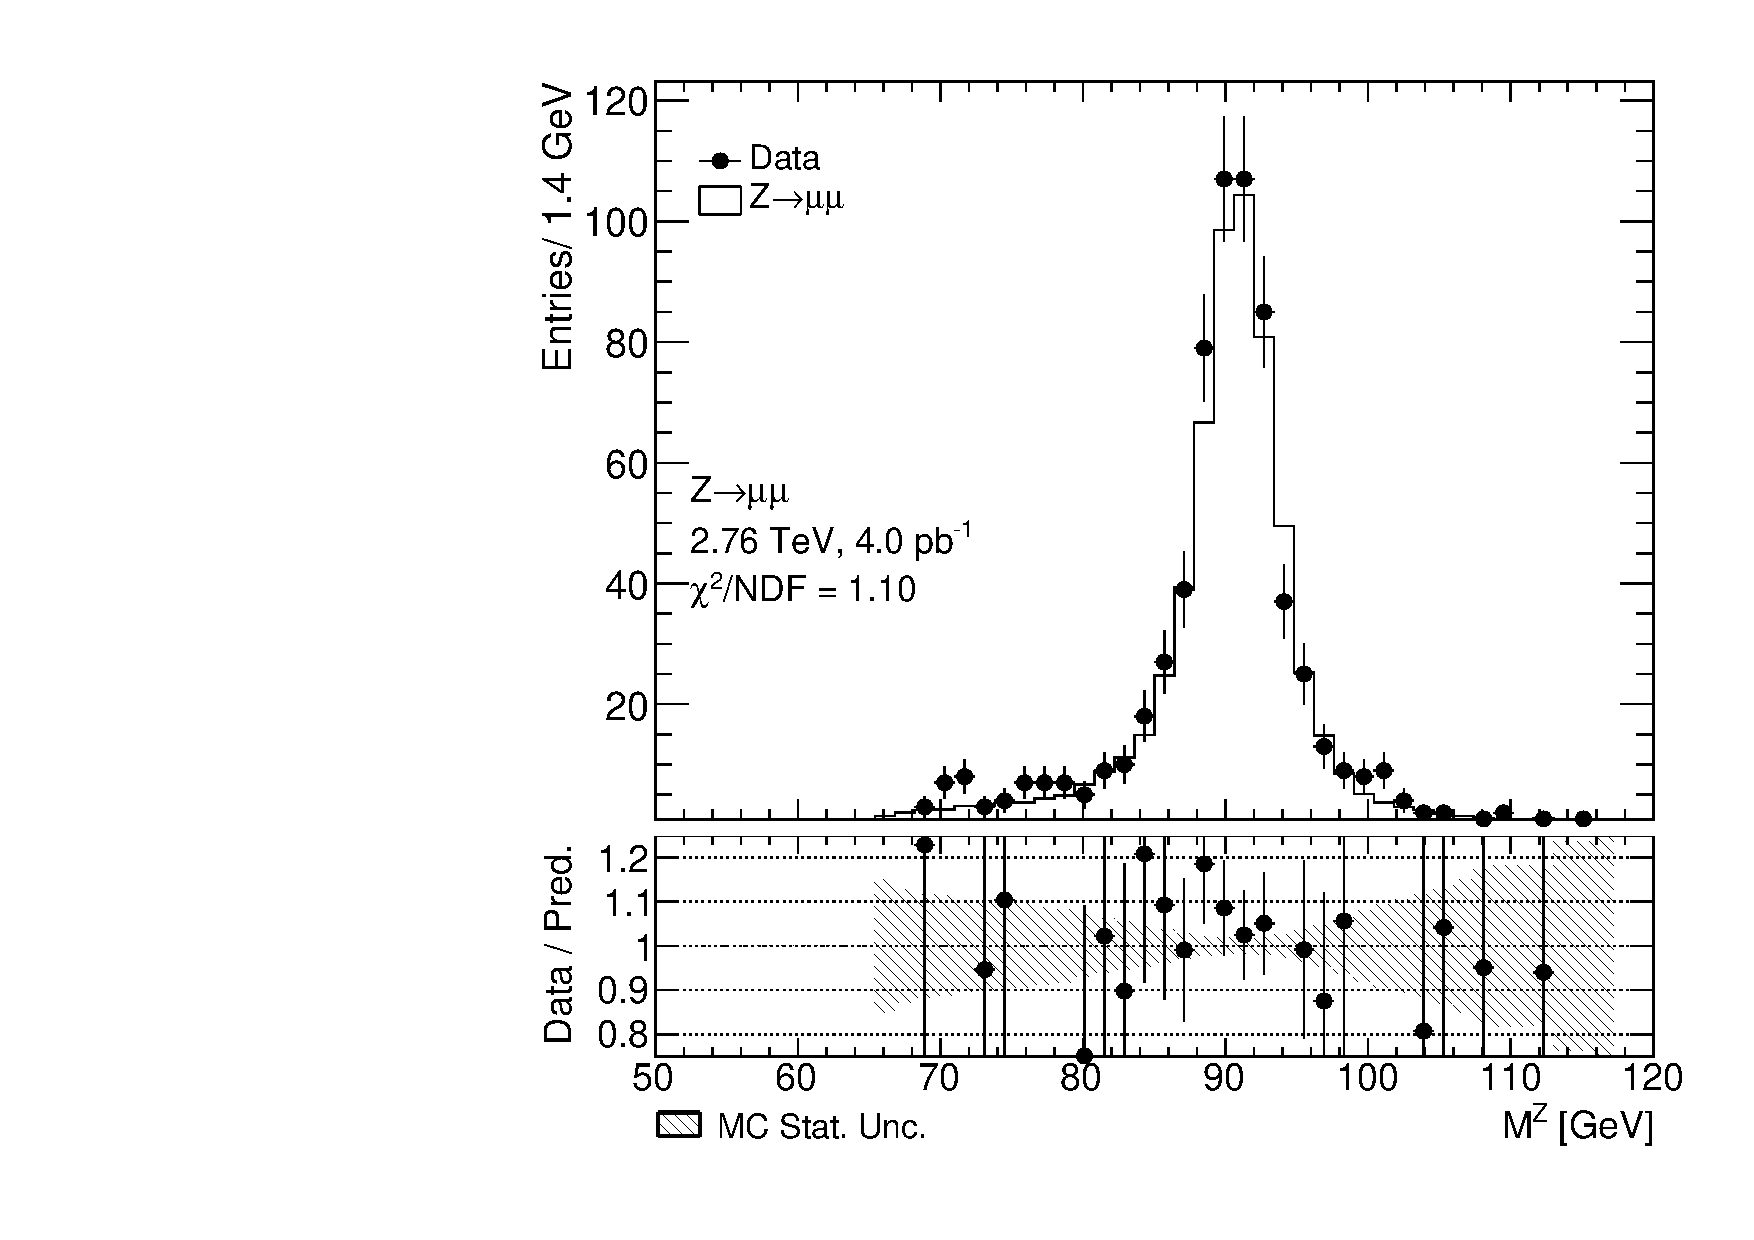
\includegraphics[width=1.\linewidth]{ControlPlots/Zanalysis/Zmumu_Boson_BosMass.pdf} \\ a)}
\end{minipage}
\caption{Dilepton mass distribution distributions from the a) $Z\to e^{+}e^{-}$ b) $Z\to \mu^{+}\mu^{-}$.}
\label{fig:CPMassZ}
\end{figure}

\begin{figure}[h]
\begin{minipage}[h]{0.49\linewidth}
\center{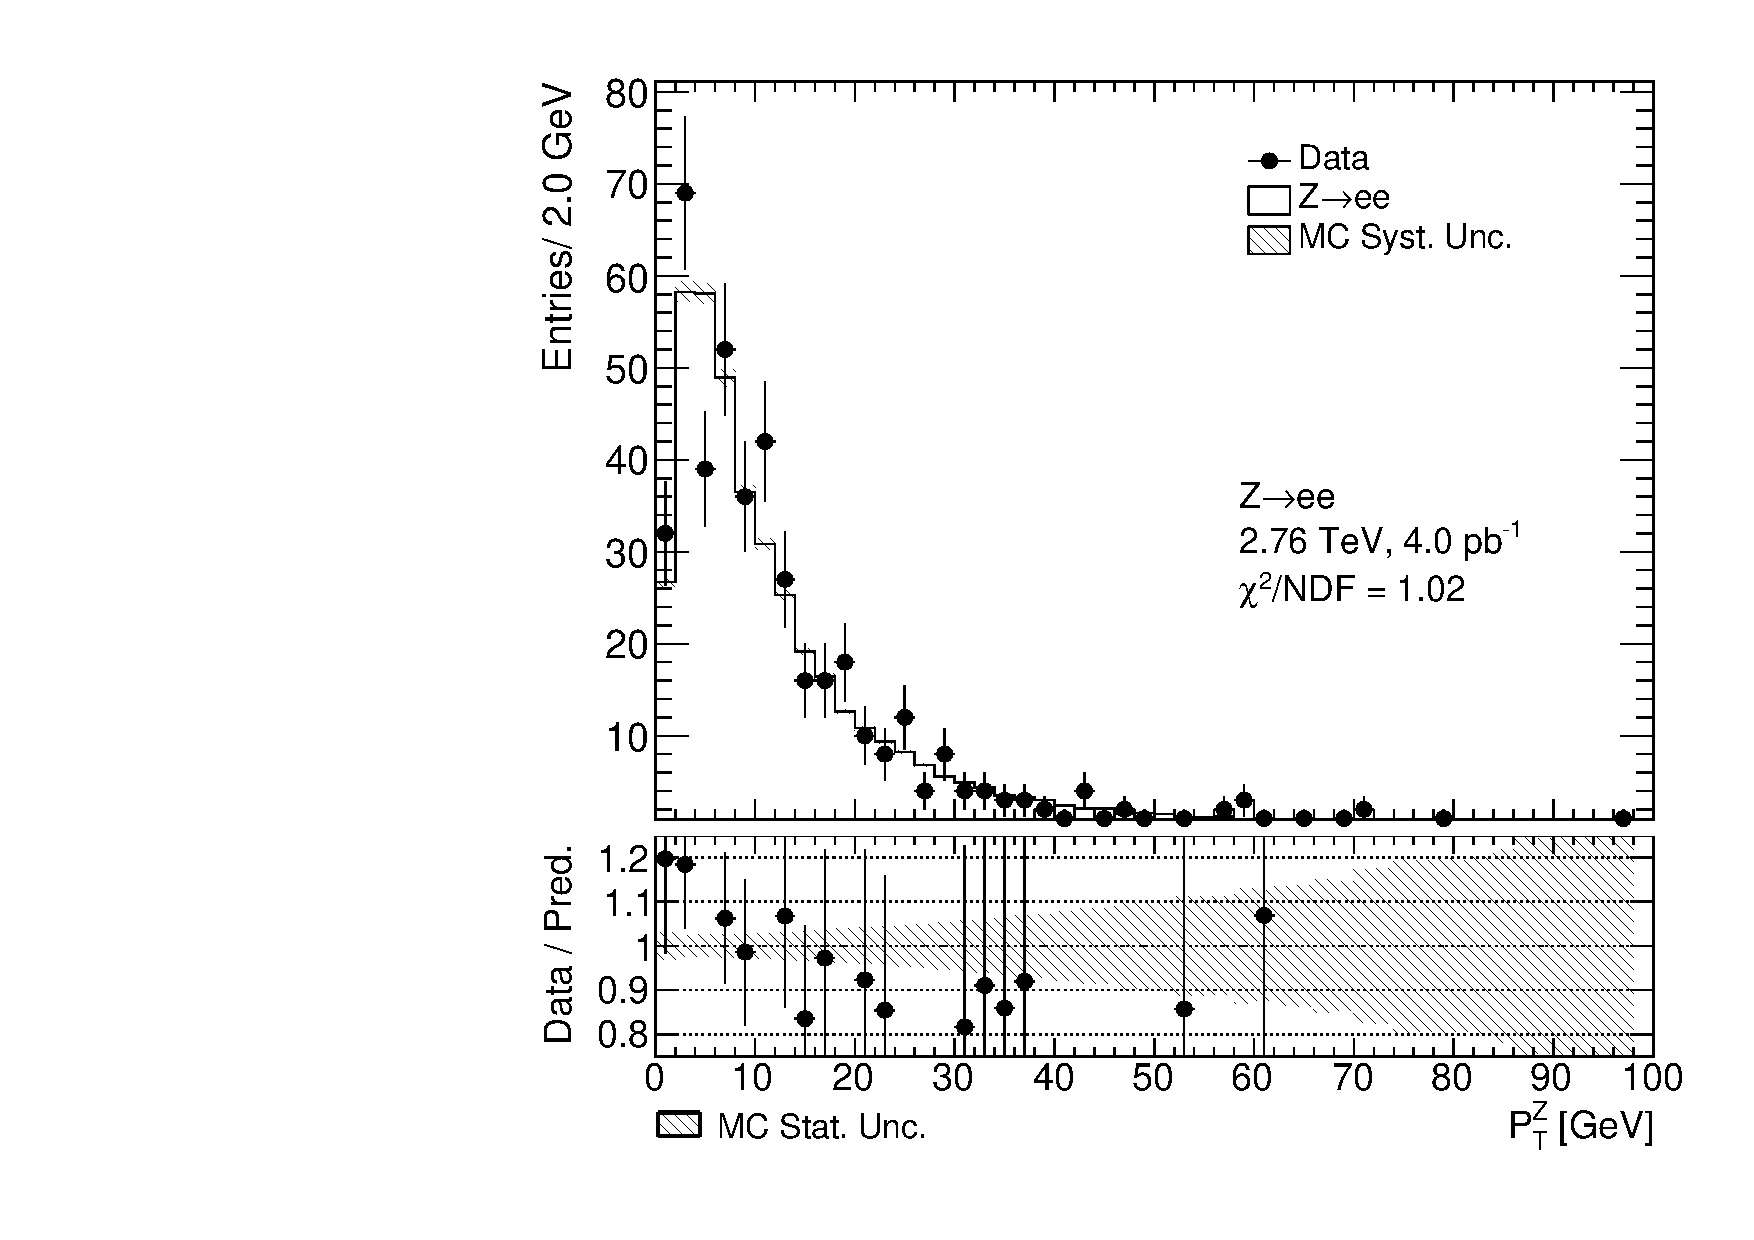
\includegraphics[width=1.\linewidth]{ControlPlots/Zanalysis/ZCC_Boson_BosPt.pdf} \\ a)}
\end{minipage}
\hfill
\begin{minipage}[h]{0.49\linewidth}
\center{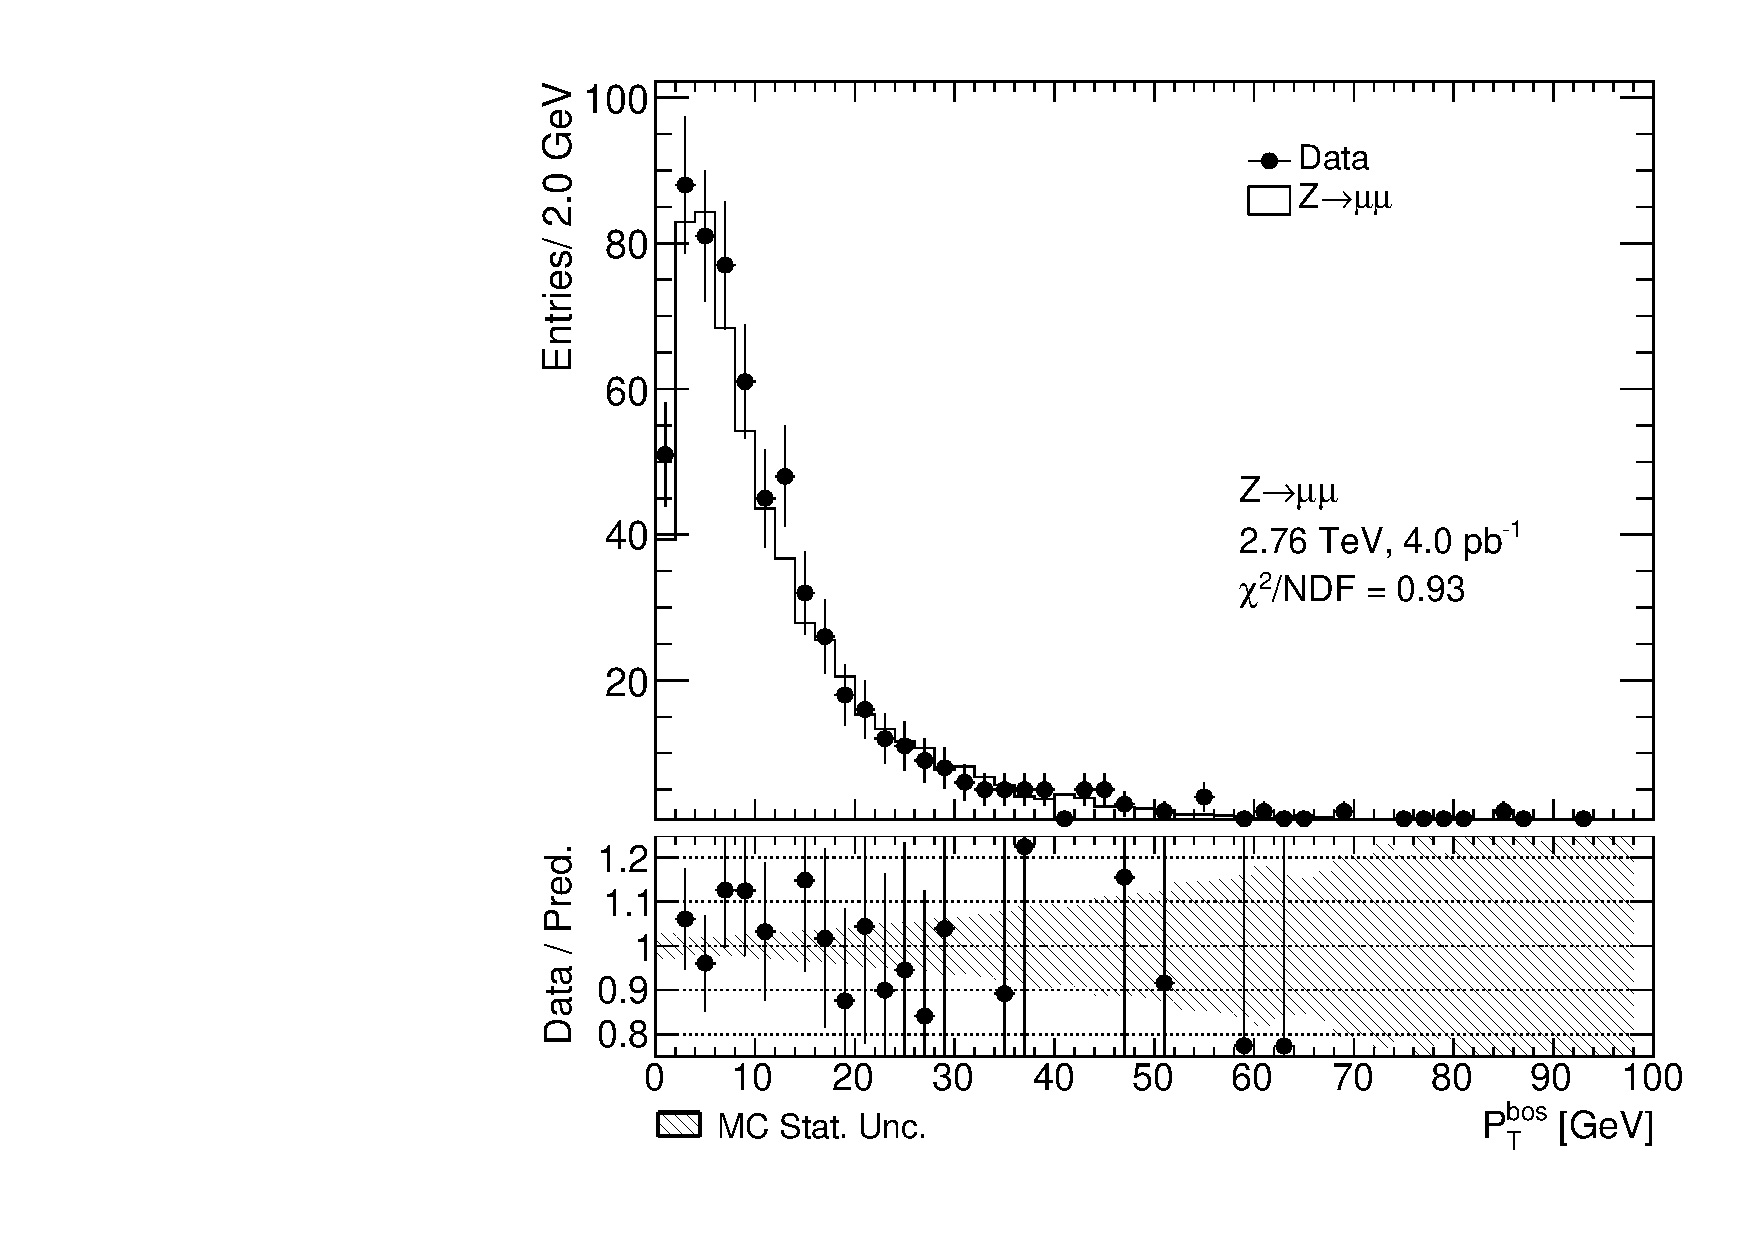
\includegraphics[width=1.\linewidth]{ControlPlots/Zanalysis/Zmumu_Boson_BosPt.pdf} \\ a)}
\end{minipage}

\caption{ Z boson transverse momentum distributions from the a) $Z\to e^{+}e^{-}$ b) $Z\to \mu^{+}\mu^{-}$.}
\end{figure}


\begin{figure}[h]
\begin{minipage}[h]{0.49\linewidth}
\center{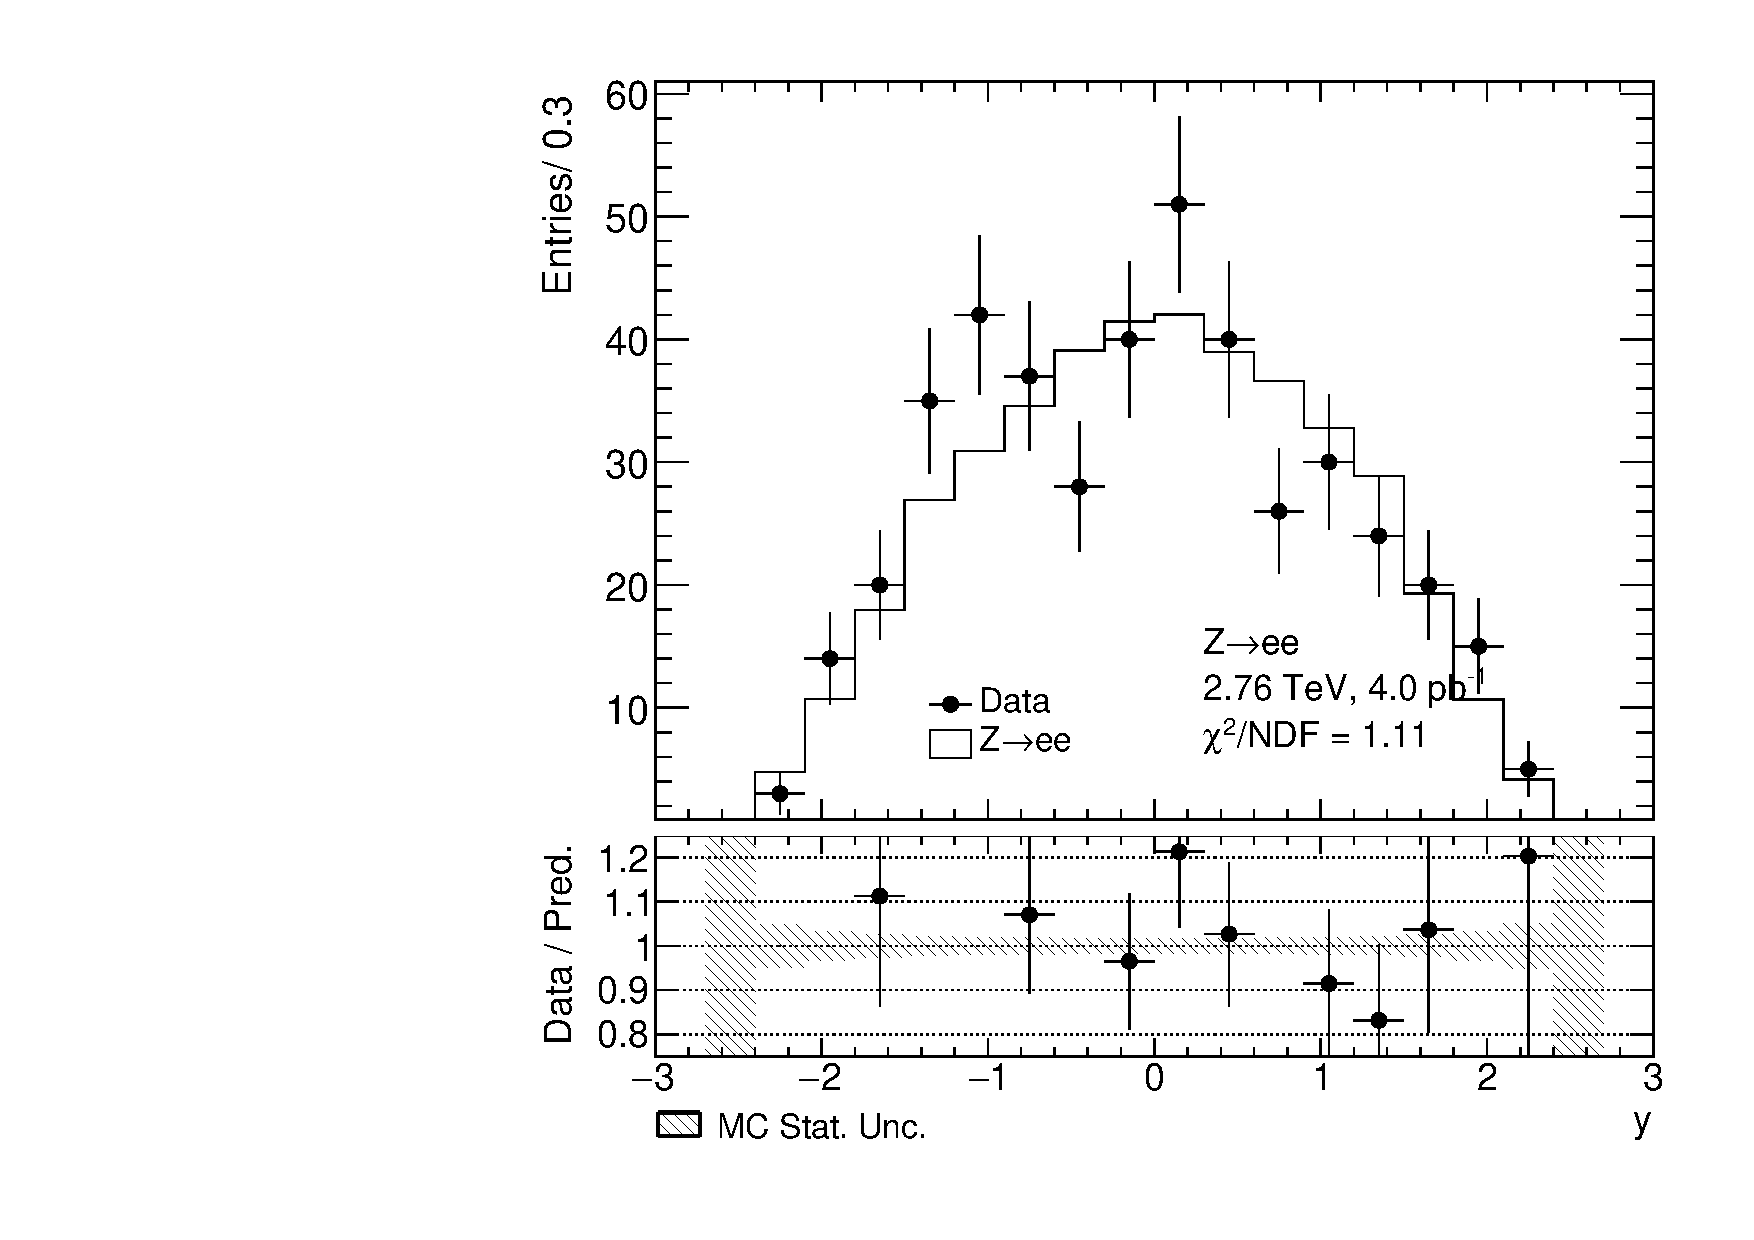
\includegraphics[width=1.\linewidth]{ControlPlots/Zanalysis/ZCC_Boson_BosY.pdf} \\ a)}
\end{minipage}
\hfill
\begin{minipage}[h]{0.49\linewidth}
\center{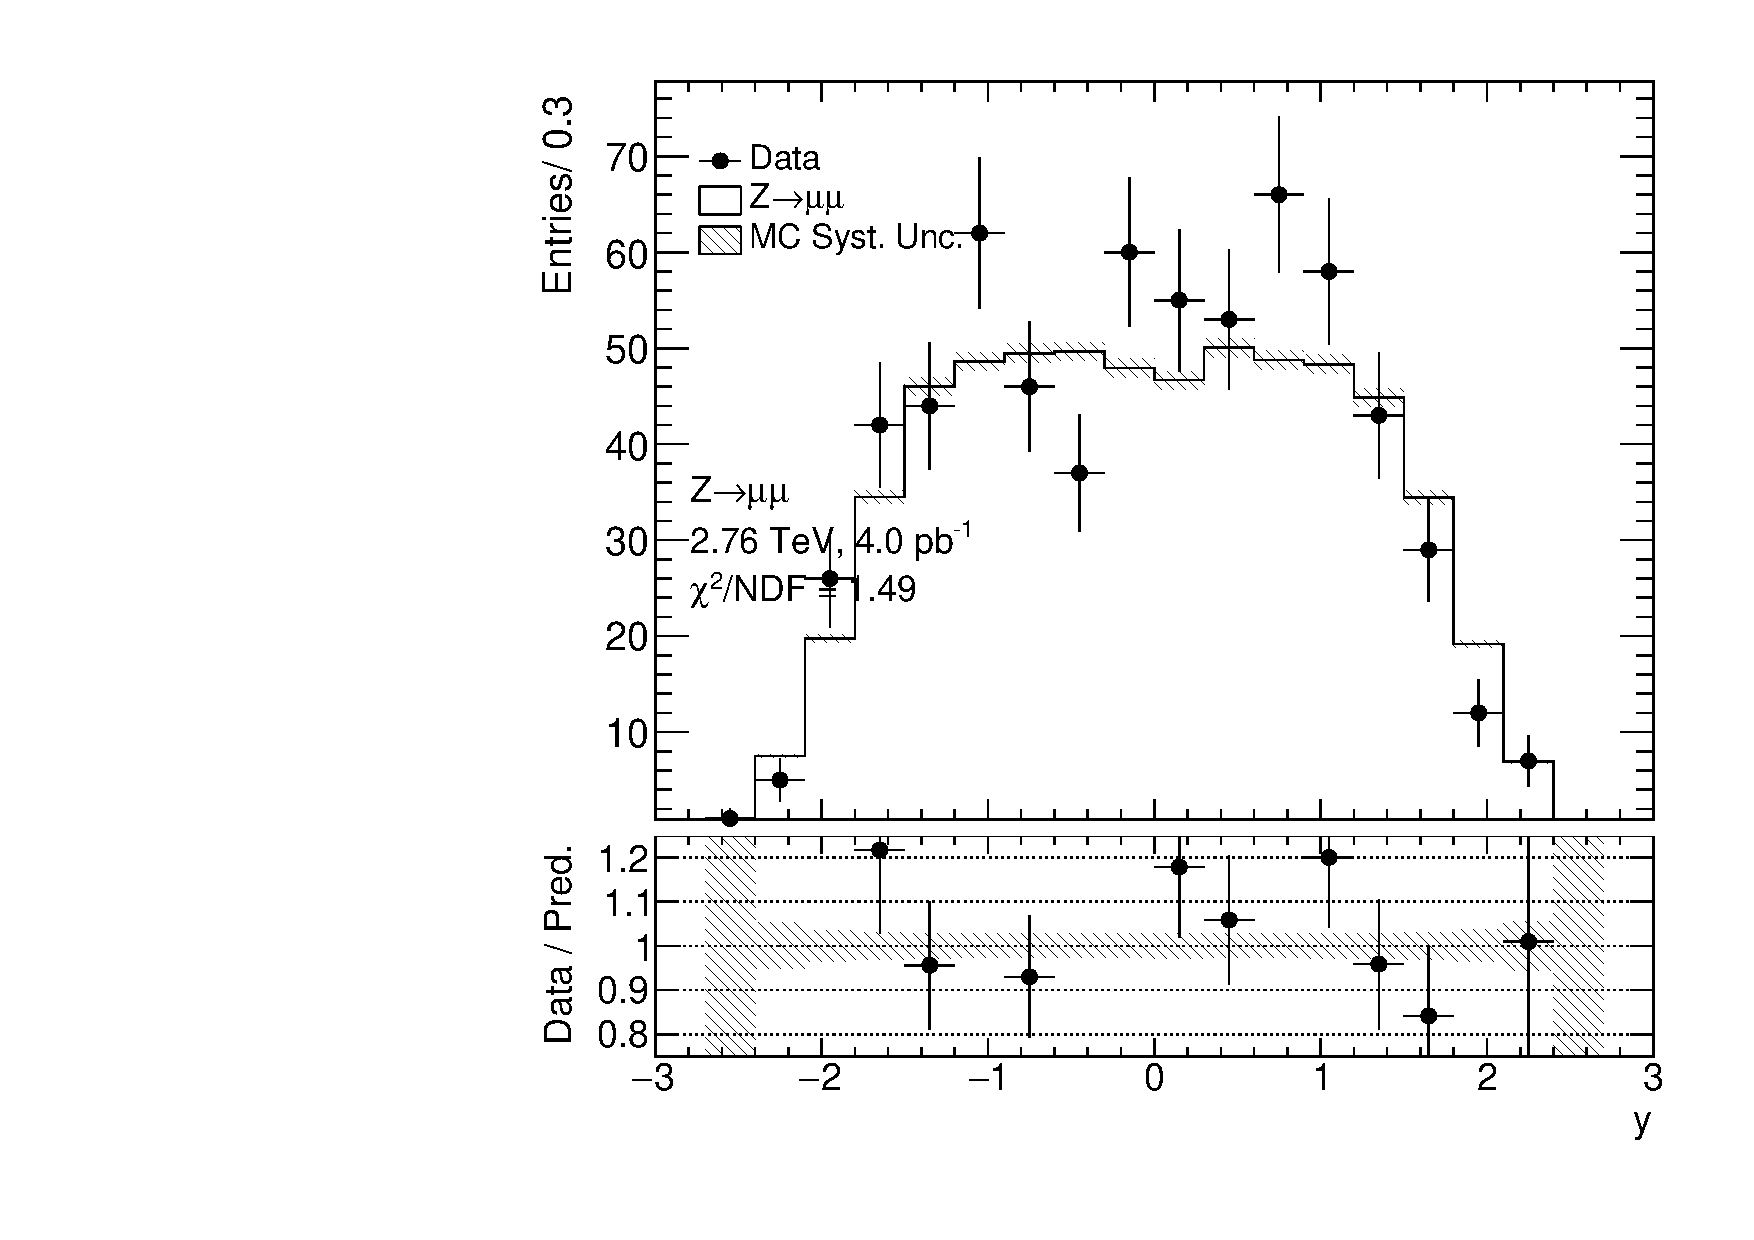
\includegraphics[width=1.\linewidth]{ControlPlots/Zanalysis/Zmumu_Boson_BosY.pdf} \\ a)}
\end{minipage}

\caption{ Z boson rapidity distribution from the a) $Z\to e^{+}e^{-}$ b) $Z\to \mu^{+}\mu^{-}$.}
\label{ris:Zll2}
\end{figure}
